\documentclass[12pt]{revtex4-2}
\usepackage{braket,amsmath,amssymb,graphicx,float,paralist,color}
\usepackage[hidelinks]{hyperref}
\allowdisplaybreaks
\begin{document}
\title{Multi-channel Kondo model URG}
\author{Abhirup Mukherjee}
\date{\today}
\maketitle
\tableofcontents
\section{Introduction of the Hamiltonian and its zero mode}
The isotropic multi-channel Kondo (MCK) model~\cite{Noz_blandin_1980,Gan_Andrei_Coleman_1993,emery_kivelson,Gan_mchannel_1994,Tsvelick_Weigmann_mchannel_1984,Tsvelick_weigmann_mchannel_1985,parcollet_olivier_large_N,kimura_taro_Su_N_kondo,PhysRevB.73.224445,cox_jarrell_two_channel_rev,affleck_1991_overscreen,Coleman_tsvelik,affleck1993exact,coleman_pepin_2003,roch_nicolas_costi_2009,schiller_avraham_2008,Durganandini_2011} is described by the Hamiltonian
\begin{align}
	\label{mc_ham}
	H = \sum_{k,\alpha,\gamma}\epsilon_{k}^\gamma \hat n^\gamma_{k\alpha} + J\sum_{kk^\prime,\gamma} \vec{S_d}\cdot\vec{s}_{\alpha\alpha^\prime}{c^\gamma_{k\alpha}}^\dagger c^\gamma_{k^\prime\alpha^\prime}~.
\end{align}
In the above equation, \(k,k^\prime\) sum over the momentum states, \(\alpha,\alpha^\prime\) sum over the spin indices and \(\gamma\) sums over the various channels. \(\vec S_d, \vec s\) are the impurity and conduction bath spin vectors. The presence of a common spin-exchange coupling \(J\) for all the channels is what makes the problem isotropic with respect to the channels.

The zero mode of this Hamiltonian is obtained by keeping only the central component of the Fourier transform of the kinetic energy part:
\begin{align}
	\epsilon(\vec r) \simeq \delta_{\vec r,0}\epsilon(\vec r = 0) \implies \epsilon_{\vec k} = \sum_{\vec r}\epsilon(\vec r) e^{i \vec{k}\cdot\vec{r}} = \epsilon(\vec r=0) = \sum_q \epsilon_{\vec q}
\end{align}
Assuming the dispersion already includes the chemical potential \(\mu\), we have 
\begin{align}
\sum_q \epsilon_{\vec q} = \rho \Delta \epsilon\sum_{\epsilon=\epsilon_F-D}^{\epsilon_F + D} \left(\epsilon - \mu\right) = \rho\Delta \epsilon\left(\epsilon_F - \mu\right)
\end{align}
If we set the chemical potential at the Fermi surface, this summation vanishes.
\begin{align}
	\epsilon_{\vec k} =  \rho\Delta \epsilon\left(\epsilon_F - \mu\right) = 0
\end{align}
and the zero mode Hamiltonian is then just the spin-exchange part of the Hamiltonian:
\begin{align}
	H_\text{zero mode} = J\sum_{kk^\prime,\gamma} \vec{S_d}\cdot\vec{s}_{\alpha\alpha^\prime}{c^\gamma_{k\alpha}}^\dagger c^\gamma_{k^\prime\alpha^\prime}~.
\end{align}
This procedure is equivalent to taking a zero-bandwidth approximation on the full Hamiltonian \cite{zitko_fabrizio_2017}; the final Hamiltonian then correspond to the degrees of freedom on the Fermi surface, and we recover the zero mode Hamiltonian again once we set the energy of the Fermi surface to zero.

We can make one more identification: the sum over the momentum space states amounts to a local state at the zeroth sites of the indicates channels: \(\sum_k {c^\gamma_{k\alpha}}^\dagger = {c^\gamma_{\vec r=0, \alpha}}^\dagger\), This suggests we shoud define spin operators for the zeroth sites of the channels:
\begin{align}
	\sum_{kk^\prime} {s}^a_{\alpha\alpha^\prime}{c^\gamma_{k\alpha}}^\dagger c^\gamma_{k^\prime\alpha^\prime} = {s}^a_{\alpha\alpha^\prime}{c^\gamma_{0\alpha}}^\dagger c^\gamma_{0\alpha^\prime} = s_\gamma^a
\end{align}
In the terms of the local spin operators \(\vec s_\gamma = (s_\gamma^x,s_\gamma^y,s_\gamma^z)\), we can define the total spin of the zero mode of the bath: \(\vec s_\text{tot} = \sum_\gamma \vec s_\gamma\) and the zero mode Hamiltonian then takes the simpler form of a star graph Hamiltonian:
\begin{align}
	\label{zeromode_ham}
	H_\text{zero mode} = J \vec{S_d}\cdot\vec{s}_\text{tot}~.
\end{align}
This star graph is shown schematically in fig.~\ref{stargraph}.

\begin{figure}[htpb]
	\centering
	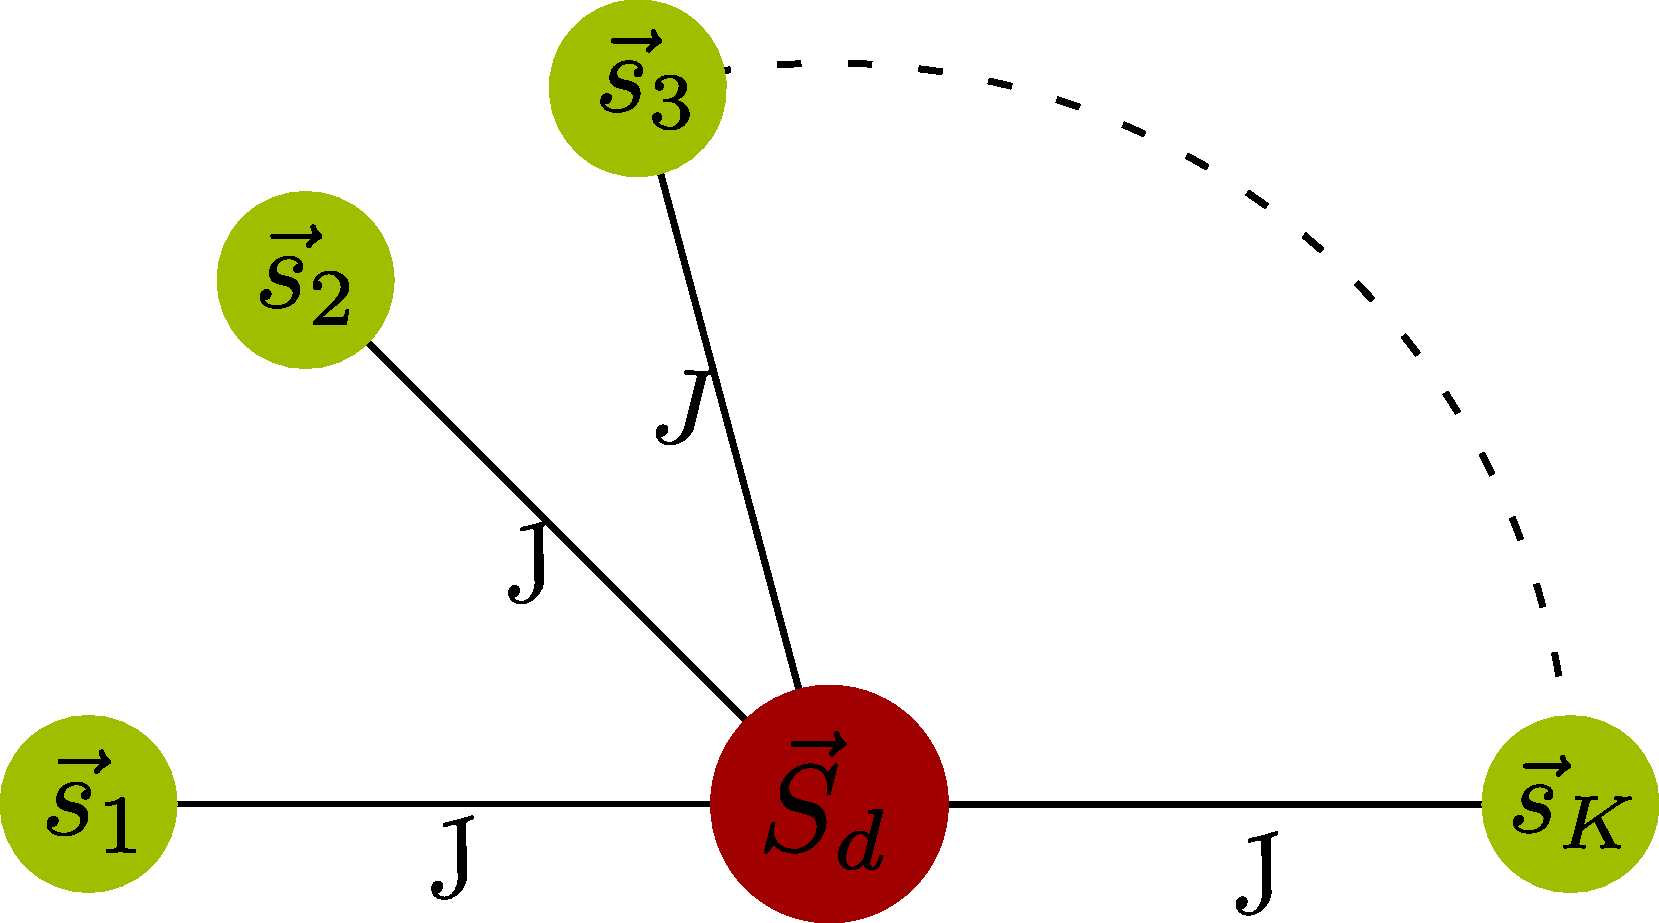
\includegraphics[width=0.3\textwidth]{./stargraph.pdf}
	\caption{Zero mode of the \(K-\)channel Kondo model, represented as a "star graph". The central red node denotes the impurity spin \(\vec S_d\), while the outer nodes denote the spins \(\vec s_\gamma\) of the zeroth sites of the channels \(\gamma=1,2,\ldots,K\). The straight lines represent the spin-exchange interaction between the central node and the outer nodes mediated by the coupling \(J\).}
	\label{stargraph}
\end{figure}

\section{Symmetries of the star graph}
This star graph commutes with a number of operators, revealing various symmetries of the problem. The first of such operators is \(s_\text{tot}^2\). Henceforth we will drop the label \(\text{zero mode}\). To see the commuation, note that \(s_\text{tot}^2\) can be written as \(s_\text{tot}^2 = \sum_{i=x,y,z}\left(s_\text{tot}^i\right)^2\). This then gives
\begin{align}
\left[s_\text{tot}^2, H\right] = \left[\sum_{i=x,y,z}{s^i_\text{tot}}^2, J \sum_{i=x,y,z} S_d^i s^i_\text{tot}\right] = \sum_{i,j}J S_d^i \left\{s_\text{tot}^i, \left[s_\text{tot}^i,s_\text{tot}^j\right]\right\} = \sum_{i,j}J S_d^i \left\{s_\text{tot}^i, i \epsilon^{ijk}s^k_\text{tot}\right\} = 0
\end{align}
The total spin angular  momentum operator \(S^2 = \left(\vec S_d + \vec s_\text{tot}\right)^2 \) also commutes with the Hamiltonian. To see this, note that we can rewrite the operator as
\begin{align}
	S^2 = \left(\vec S_d + \vec s_\text{tot}\right)^2 = \frac{3}{4} + s^2_\text{tot} + \frac{2}{J} H
\end{align}
Since we already know that \(s_\text{tot}\) commutes with \(H\), we have that \(\left[S^2, H\right] = 0\). The \(z-\)component of this total spin operator also commutes with the Hamiltonian:
\begin{align}
	\left[S^z, H\right] = \left[S^z, J \left(\frac{1}{2}S^2 - \frac{3}{8} - \frac{1}{2}s_\text{tot}^2\right) \right]  = \frac{J}{2}\left(\left[S^z, S^2\right] - \left[s_\text{tot}^z, s_\text{tot}^2\right] \right) = 0
\end{align}

One final operator that we will look at is the spin parity operator \(\pi^a = \sigma_d^a \otimes_{i=1}^K \sigma_i^a\).
\begin{align}
	\left[H, \pi^a\right] = J\sum_{b,j} \left[S_d^b s_j^b, \sigma_d^a \otimes_{i=1}^K \sigma_i^a\right] = \sum_{bj}\left(S_d^b \sigma_d^a s^b_j \sigma^a_j - \sigma_d^a S_d^b \sigma^a_j s^b_j\right) \otimes_{i<j}\sigma_i^a \otimes_{i>j}\sigma^a_i = 0
\end{align}

\section{Eigenvalues and eigenstates of the star graph}
The star graph can be diagonalized. Since the Hamiltonian commutes with \(s_\text{tot}^2\), it is already block-diagonal in the quantum number \(s_\text{tot}\). Let us represent the quantum number of \(s_\text{tot}^z\) by \(m\). For a particular \(s_\text{tot}\), \(m\) can take values from the set \(\left[-s_\text{tot}, s_\text{tot}\right] \). The spin \(S_d^z\) can also take values \(\pm \frac{1}{2}\). From now on, we will assume we are in the subspace of a particular \(s_\text{tot} = M\), so we will ignore that quantum number and write the kets simply as \(\ket{S_d^z, m}\). So, the notation \(\ket{\uparrow,-1}\) means the state with \(S_d^z = \frac{1}{2}\) and \(m = -1\). We will now show that even inside the block of \(2\times s_\text{tot}\) (or \(2\times s_\text{tot} + 1\), depending on whether it is odd or even) defined by a particular value of \(s_\text{tot}\), the Hamiltonian actually separates into decoupled \(2\times 2\) blocks. To see why, first note that the terminal states \(\ket{\downarrow, -M}\) and \(\ket{\uparrow, M}\) are already eigenstates, because they cannot scatter (the impurity can only flip down, and this would require the bath to flip up, but \(s^z_\text{tot}\) is already at its maximum value \(M\)). The other \(2M - 2\) states can be organized into \(2\times 2\) blocks formed by the states \(\ket{\uparrow, m}\) and \(\ket{\downarrow, m+1}\) for \(m \in \left[-M, M-1\right] \). The fact that this block does not interact with the other blocks can be easily verified: if there was some other state which when acted upon by the Hamiltonian gave a non-zero projection on \(\ket{\uparrow, m}\), it would have to come from \(S_d^z = \downarrow\), and this would mean the bath spin would have had to flip down. This means the bath spin in that state would have to be \(m+1\), and that is precisely the other state in the block. 

Defining \(x^M_m = M(M+1) - m(m+1)\), the \(2\times 2\) blocks can be written as
\begin{align}
	H_m = \begin{pmatrix} \frac{Jm}{2} & \frac{J}{2}\sqrt{x^M_m} \\ \frac{J}{2}\sqrt{x^M_m} & -\frac{J}{2}(m+1) \end{pmatrix} , m \in \left[-M, M-1\right] 
\end{align}
The eigenvalues are 
\begin{align}
	% \label{eigenvalue}
	\lambda_{\pm}^{M} = - \frac{J}{4} \pm \frac{J}{2}\left(M + \frac{1}{2}\right) 
\end{align}
The eigenvalues of the terminal states are \(\frac{JM}{2}\). The set of eigenvalues \(\lambda^{M_\text{max}}_-\) form the ground state subspace \(\left\{ \ket{\Psi^M_{m,-}} \right\} \) of degeneracy \(2M_\text{max} = K\). This common \(K-\)fold degenerate eigenvalue is \(-\frac{J}{2}(M+1)\).
The normalized eigenstates of the \(2\times 2\) blocks for each value of \(m\) are given by
\begin{align}
	\ket{\Psi^M_{m,-}} &= \frac{1}{\sqrt{(M+m+1)(1+2M)}}\left[-\sqrt{x_m^M}\ket{\uparrow, M, m} + \left(M + m + 1\right)\ket{\downarrow,M,m+1}\right],& m \in \left[-M, M-1\right] \\
	\ket{\Psi^M_{m,+}} &= \frac{1}{\sqrt{(M -m)(M - m + 1)}}\left[\sqrt{x_m^M}\ket{\uparrow, M, m} + \left(M - m\right)\ket{\downarrow,M,m+1}\right],& m \in \left[-M, M-1\right]
\end{align}
Note that the index \(m\) that we are using to label the eigenvalues is actually related to a conserved quantity; the total spin operator along \(z\), \(S^z\). That is, the eigenstates \(\ket{\Psi^M_{m,\pm}}\) have \(S^z = S_d^z + s_\text{tot}^z = m + \frac{1}{2}\).

\section{Role of the star graph in determining the physics of the problem}
Methods like CFT, Bethe ansatz, bosonization and NRG~\cite{affleck_1991_overscreen,Tsvelick_Weigmann_mchannel_1984,Gan_mchannel_1994,pang_cox_1991,emery_kivelson,vondelft_prl_1998} have shown that \textit{neither the weak coupling nor the strong coupling Hamiltonians are stable fixed points of the MCK models}. Instead, the RG flows converge to an intermediate coupling fixed point. The RG flows \textit{preserve the degeneracy of the ground state}~\cite{pang_cox_1991,kroha_kolf_2007,zitko_fabrizio_2017}\textcolor{red}. For example, the two-channel and the three-channel Kondo models have ground state degeneracies of 2 and 3 respectively, throughout the RG flow. Analytic and numerical studies also showed that \textit{the two and three-channel models enjoy a weak-strong duality}~\cite{kroha_kolf_2007,zitko_fabrizio_2017}: the model at strong coupling, when projected onto the ground state basis, can also be thought of as a Kondo model at weak coupling, but possibly with a modified central spin. For example, in the two channel Kondo model, the model at strong coupling can be mapped onto the same model with a small coupling parameter, but with the central Kondo spin-half impurity replaced by a new, composite spin-half object formed by the doubly-degenerate ground state of the strong coupling model~\cite{kroha_kolf_2007}. The strong and weak coupling models are formally identical and the model is self-dual. The case of the three-channel model is different~\cite{zitko_fabrizio_2017} because there, the central impurity gets replaced by a new \textit{spin-1} impurity formed by the triply-degenerate ground state. Compared to the self-duality of the two-channel model, this case corresponds to a cross duality between a spin-\(\frac{1}{2}\) and a spin-1 model. We will now show that these qualitative features can be captured very simply by the star graph.

At weak coupling \(J \to 0^+\), the central spin is weakly coupled to the outer spins and can freely flip like a local moment. \textit{This makes it prone to screening because of the \(s^\pm\) terms in the star graph}. At strong coupling \(J \to \infty^-\), the outer spin-half objects tightly bind with the central spin-half object to form a single spin. The remaining states in the conduction bath channels form new zero modes and create a new outer ring of spins that interact with the new central spin, \textit{leading to another MCK problem with a new and small exchange coupling which is RG relevant, so the strong coupling fixed point \(J \to \infty^-\) is unstable}. This shows that it can be argued, even from the star graph, that the two limits of the model cannot be stable fixed points, and the actual fixed point has to lie somewhere in between.

The star graph conserves the total spin \(S^z\), and this leads to a \(K-\)fold degeneracy in the ground state of the \(K-\)channel spin-half star graph. Since \(S^z\) commutes with the star graph, the ground states are eigenstates of \(S^z\) with distinct eigenvalues \(\frac{K+1}{2}, \frac{K-1}{2},\ldots,\frac{-K-1}{2}\). \textit{This feature - the equality of energy eigenvalue for distinct values of \(S^z\) - persists for all values of \(J \in \left[0^+, \infty^-\right]\)}. This is because, the gap between the degenerate subspace and the next excited level is \(J\) or \(\frac{J}{2}\), depending on whether \(K\) is even or odd, and the gap is always non-zero as long as \(J\) lies in the regime of RG flow. In other words, as the exchange coupling grows(shrinks) from \(0^+\left(\infty^-\right)\) towards the fixed point value \(J^*\), the degeneracy remains protected at \(K\). This is qualitatively different from the case of the single-channel Kondo model; there, the \(2-\)fold degeneracy of the local moment fixed point crosses over into a stable and unique singlet ground state at low temperatures/energies.

It can be demonstrated very simply that the ground state degeneracy of the star graph lies at the heart of the MCK problem. It can be argued that the ground state degeneracy of the more general MCK model with a spin-\(S\) impurity is given by \(d(S) = |K - 2S|+1\). This is because, if we write the star graph Hamiltonian in eq.~\ref{stargraph} as \(H = J\left[J^2 - S_d^2 - s^2_\text{tot}\right] \) (where \(\vec J = \vec S_d + \vec s_\text{tot}\)), we can see that the ground state is realized when \(s_\text{tot}\) and \(S_d\) takes their maximum values of \(S\) and \(\frac{K}{2}\) respectively, and \(J\) takes its corresponding minimum value of \(|\frac{K}{2} - S|\). For this value of \(J\), \(J^z\) can take \(2J+1 = |K - 2S|+1\) values, and since the Hamiltonian (and hence the ground state energy) depends only on \(J\) and not on \(J^z\), all these \(2J+1\) states labelled by the distinct quantum numbers are degenerate. If we now ask when the degeneracy is exactly unity, we get the condition \(K=2S\). The cases of multiple degeneracy lie either in \(K>2S\) or \(K<2S\). The case of \(K=2S\) is that of exact screening, where we know that the ground state is a singlet described by a local Fermi liquid phase \cite{wilson1975,nozieres1974fermi,Noz_blandin_1980,andreiKondoreview,tsvelickKondoreview}~\cite{Noz_blandin_1980,Gan_Andrei_Coleman_1993,emery_kivelson,Gan_mchannel_1994,Tsvelick_Weigmann_mchannel_1984,Tsvelick_weigmann_mchannel_1985,parcollet_olivier_large_N,kimura_taro_Su_N_kondo,PhysRevB.73.224445,cox_jarrell_two_channel_rev,affleck_1991_overscreen,Coleman_tsvelik,affleck1993exact,coleman_pepin_2003,roch_nicolas_costi_2009,schiller_avraham_2008,Durganandini_2011}. The cases of \(K>2S\) and \(K<2S\) correspond to over-screened and under-screened systems, both of which are known to exhibit non-Fermi liquid behaviour. This shows that the ground state degeneracy can be used to classify the low energy phases into Fermi liquids and non-Fermi liquids.

The fact that the strong coupling fixed point can be seen as a new star graph problem with a modifed central spin reveals the duality mentioned before. At strong coupling \(J \gg 1\), we can obtain a new star graph by defining a new spin-\(\left(\frac{K-1}{2}\right)\) object from the \(K-\)fold degenerate ground state manifold and letting this interact with the new outer spins formed by the remaining sites of the conduction channels. This new interaction is generated by the minimal hopping that exists between the zeroth site and the first sites of each of the conduction bath channels, and is characterised by the small superexchange coupling \(J^\prime \sim t^2/J\). \textit{The conclusion is that a large \(J\) model with a central spin-half object can be transformed into a small \(J^\prime\) overscreened model with a central spin-\(\left(\frac{K-1}{2}\right)\) object}. This is shown schematically in Fig.~\ref{duality_fig}. The former is RG irrelevant while the latter is relevant, both flowing towards the stable fixed point \(J = J^\prime = J^*\). For \(K=2\), the central spin for the \(J^\prime\)-problem is of size \(\frac{K-1}{2} = \frac{1}{2}\), which is the same as the \(J\)-problem, so the models are self-dual, as mentioned previously.

\begin{figure}[htpb]
	\centering
	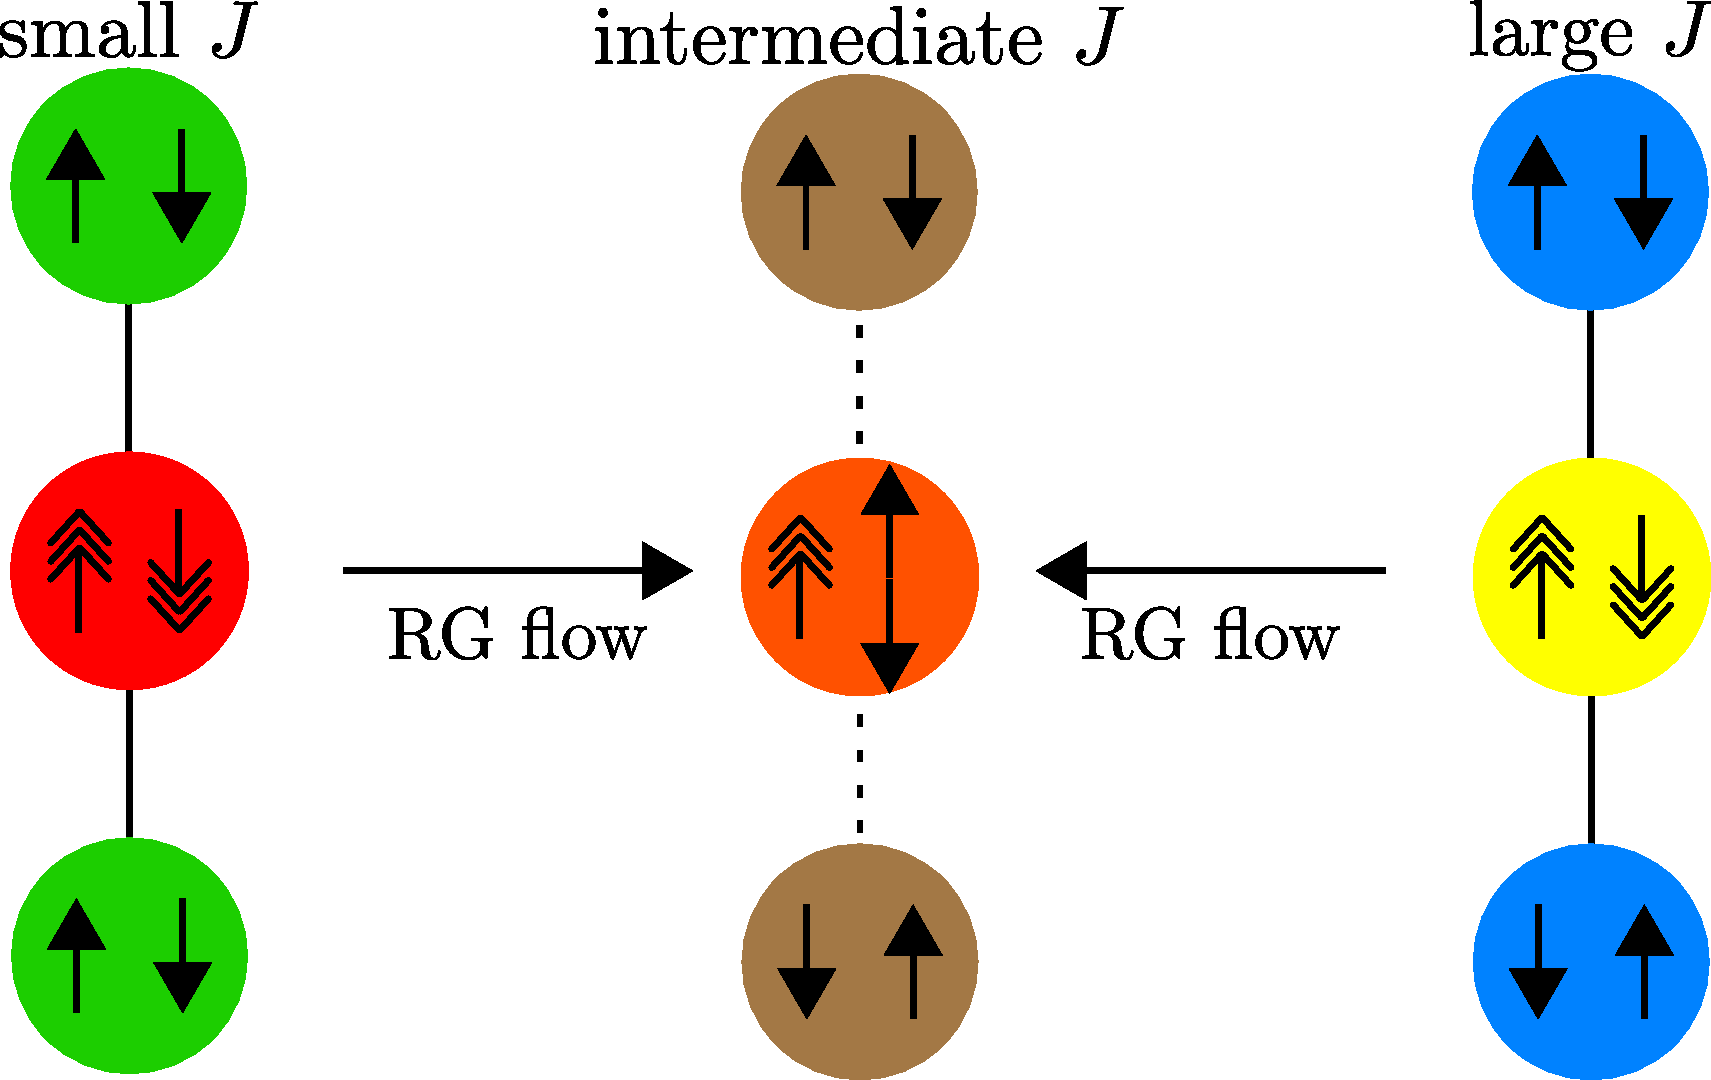
\includegraphics[width=0.45\textwidth]{./duality.pdf}
	\caption{Duality of the RG flows as seen in the star graph Hamiltonian. The red and green circles represent the impurity and zeroth site spins respectively. At large \(J\), the red circle binds with the green circles to form an effective spin \(\frac{K-1}{2}\) object (yellow) that interacts with the remaining spin of the conduction bath (blue circles). The fixed point consists of the red (purple) and green (yellow) circles binding to form a doubly degenerate ground state (orange) that interacts with the star graph of the remaining sites (brown) through the hopping.}
	\label{duality_fig}
\end{figure}

\subsection{Degree of compensation: a measure of the frustration}
One can quantify the amount of screening of the local moment at the impurity site by defining a degree of compensation \(\kappa\). Such a quantity also measures the inherent singlet frustration in the problem: the higher the degree of compensation, the better the spin can be screened into a singlet and lower is the frustration. It is given by the antiferromagnetic correlation existing between the impurity spin and conduction electron channels:
\begin{equation}\begin{aligned}
	\Gamma \equiv - \left< \vec{S_d}\cdot \vec{s}_\text{tot}\right>
\end{aligned}\end{equation}
where \(\vec s_\text{tot} = \sum_l \vec s_l\). The expectation value is calculated in the ground state. Since the inner product is simply the ground state energy of a spin-\(S\) impurity \(K-\)channel MCK model in units of the exchange coupling \(J\), we have
\begin{equation}\begin{aligned}
	\Gamma = \frac{1}{2} \left[ l_\text{imp}^2 + l_c^2 - g^S_K\left( g^S_K - 1 \right)\right]
\end{aligned}\end{equation}
\(l_\text{imp}^2 = S(S+1)\) is the length-squared of the impurity spin. Similarly, \(l_c^2 = \frac{K}{2}\left(\frac{K}{2} + 1\right) \) is the length-squared of the total conduction bath spin. \(g^S_K = |\frac{K}{2} - S| + 1\) is the ground state degeneracy. We will explore the three regimes of screening by defining \(K = K_0 + \delta, S = \frac{K_0}{2} - \delta\). \(\delta=0\) represents the exactly-screened case of \(K = 2S = K_0\). Non-zero \(\delta\) represents either over- or under-screening. In terms of \(K_0\) and \(\delta\), the degree of compensation becomes
\begin{equation}\begin{aligned}
	\label{gamma}
	\Gamma = \frac{1}{4}\left[\left( K_0 + 1 \right) ^2 - \left(|\delta| + 1 \right) ^2\right] 
\end{aligned}\end{equation}
\textit{For a given \(K_0\), the degree of compensation is maximised for exact screening \(\delta=0\), and is reduced for \(\delta \neq 0\). This shows the inability of the system to form a unique singlet ground state and reveals the quantum-mechanical frustration inherent in the zero mode Hamiltonian and therefore in the entire problem.} The degree of compensation is symmetric under the Hamiltonian transformation \(\delta \to -\delta\), and this represents a duality transformation between over-screened and under-screened MCK models. This topic will be discussed in more detail later.
\begin{figure}[htpb]
	\centering
	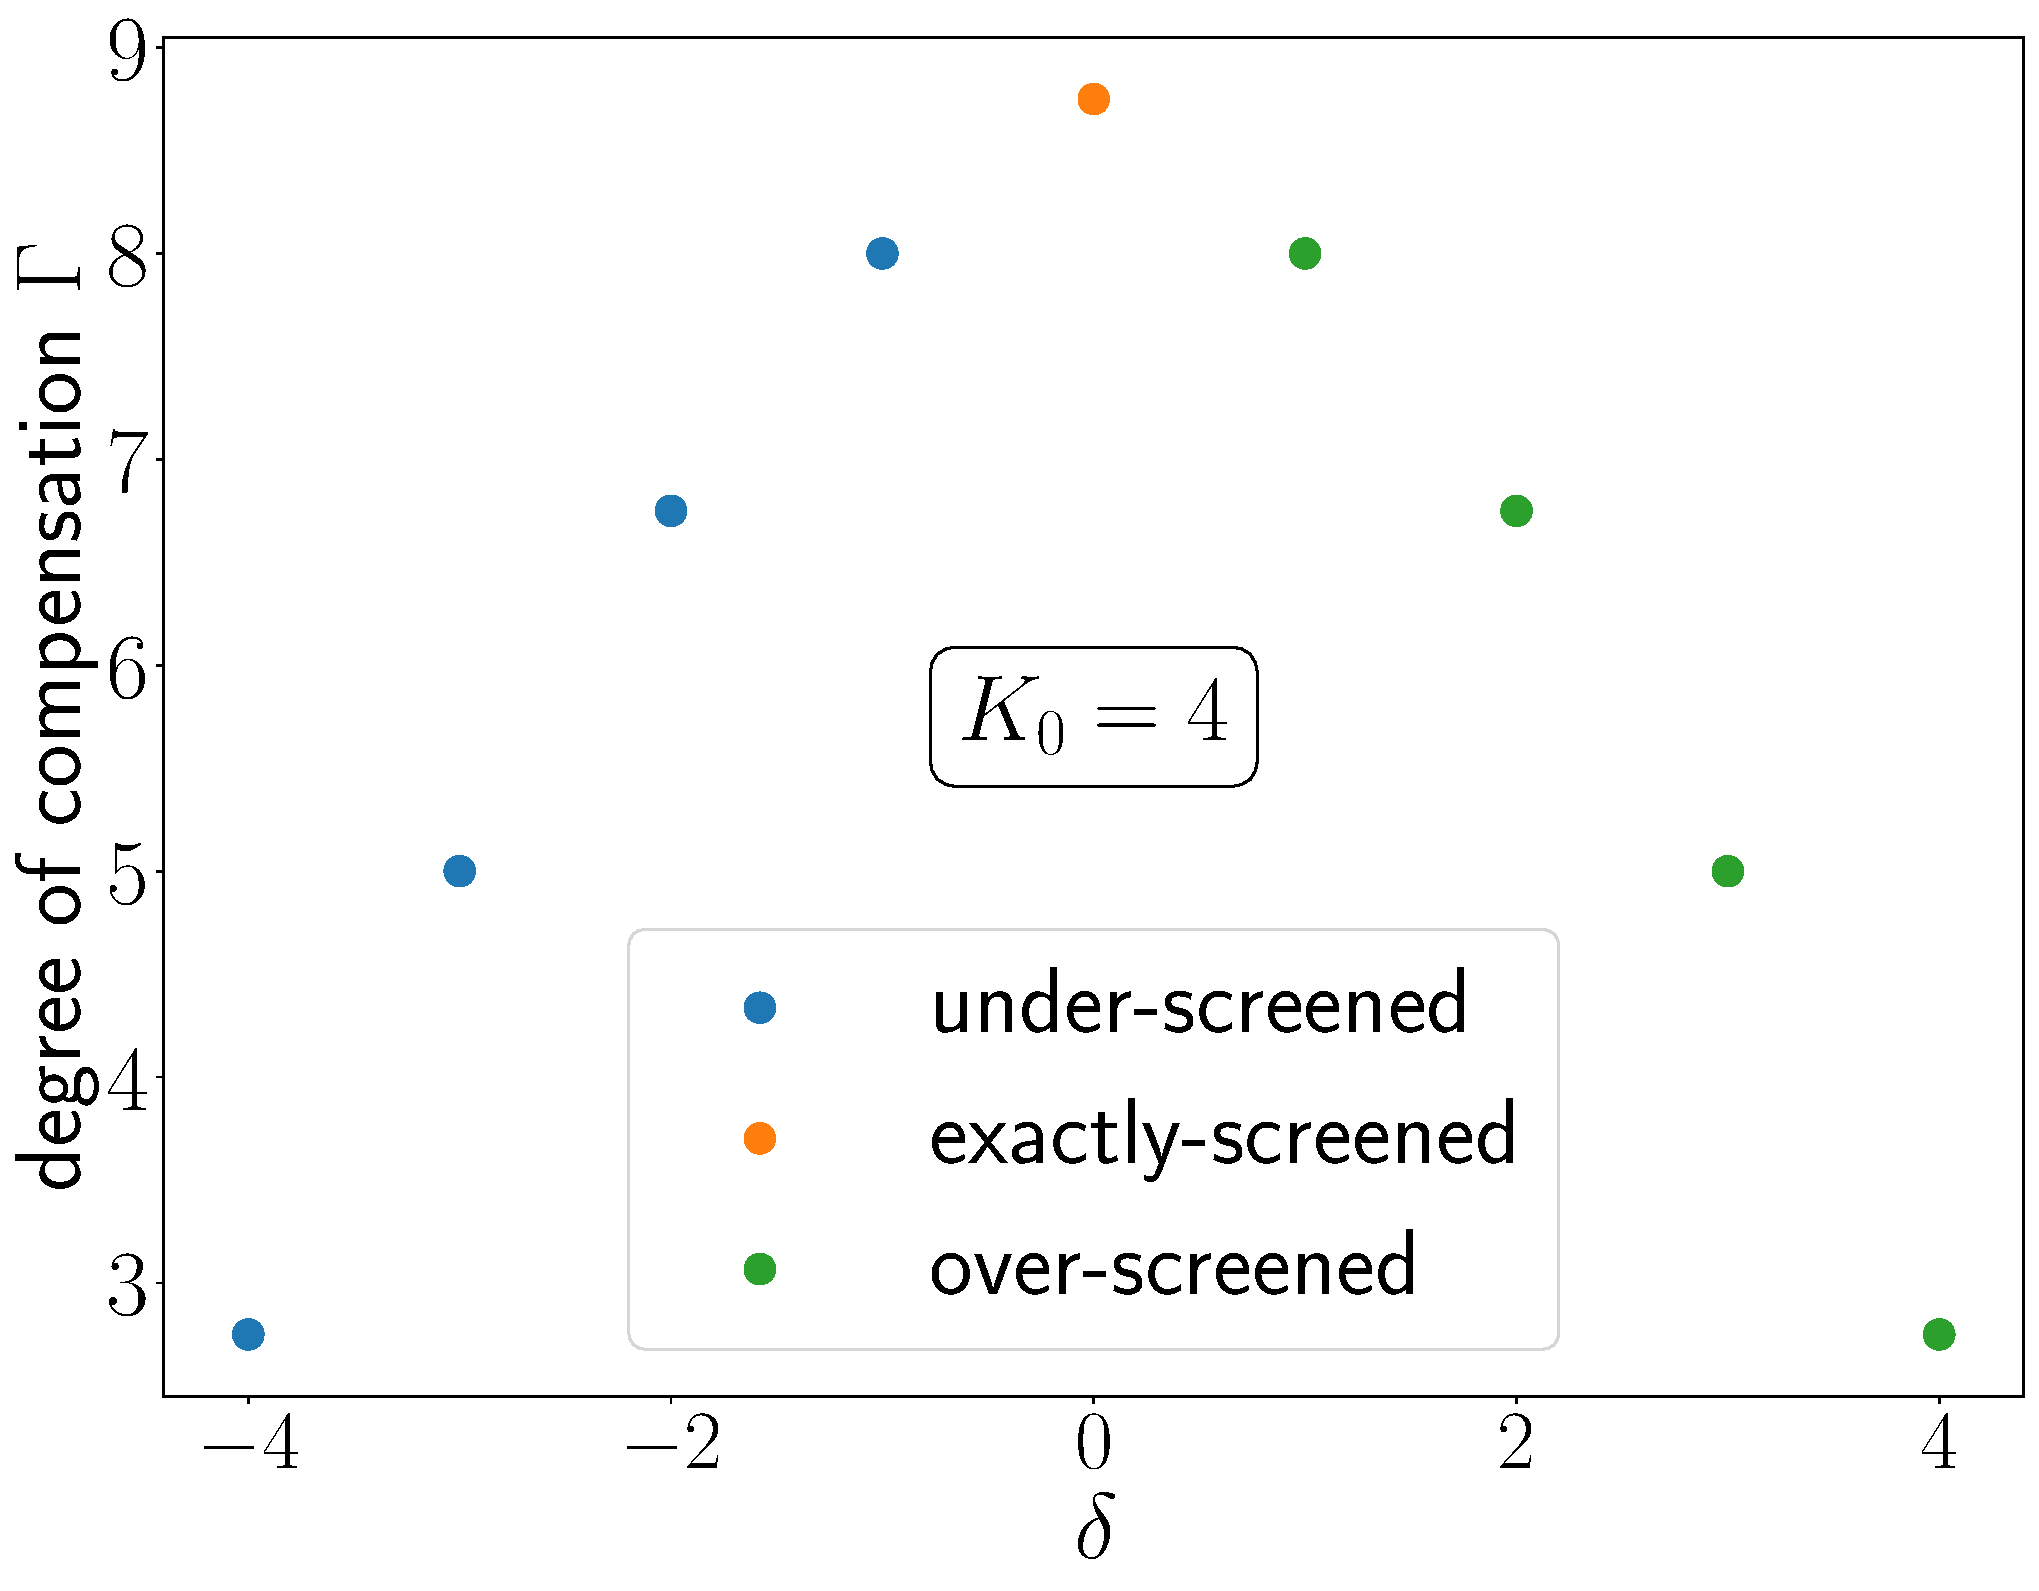
\includegraphics[width=0.45\textwidth]{../numerics/deg_of_comp.pdf}
	\caption{Variation of the degree of compensation as we tune the system from under-screening to over-screening. The maximum spin compensation occurs at exact-screening \(\delta=0\).}
\end{figure}

\section{Parity operators and impurity magnetization}

\subsection{Action of \(\pi^x\)}
We can also use the eigenvalues of \(\pi^z\) to label the eigenstates. We have the eigenvalue relation \(\pi^z \ket{S^z} = (-1)^{S^z - \frac{1}{2}}\ket{S^z}\). Applying \(\pi^z\) on these eigenstates gives
\begin{align}
	\pi^z\ket{\Psi^M_{m,-}} = \left( -1 \right) ^{m}\ket{\Psi^M_{m,-}}
\end{align}
This shows that the operator \(\pi^z\) splits the \(K-\)fold degenerate ground state manifold into two sub-manifolds of \(\pi^z\) parity \(\pm 1\). The odd values of \(m\) form the negative parity sector \(\pi^z = -1\) while the even values form the positive parity sector \(\pi^z = 1\).

It is interesting to calculate the action of the parity operator \(\pi^x\) on these eigenstates. We can write that operator as
\begin{align}
	\pi^x = (S_d^+ + S_d^-)\otimes_{i=1}^K \left(s_i^+ + s_i^-\right) 
\end{align}
We can write the simultaneous eigenstates of \(s^2_\text{tot}\) and \(s_\text{tot}^z\) in terms of the eigenstates of \(s_i^z\) using their Clebsch-Gordon coefficients:
\begin{align}
	\ket{M,m} = \sum_{\left\{m_i\right\}\atop{\sum_i m_i = m}}\ket{m_1,m_2,...,m_K} C_{\left\{m_i\right\},m,M}
\end{align}
The state \(\ket{M,m}\) is defined by \(s_\text{tot}^2\ket{M,m} = M(M+1), s^z_\text{tot}\ket{M,m} = m\). The Clebsch-Gordon coefficients are defined as \(C_{\left\{m_i\right\},m,M} = \braket{m_1,m_2,...,m_K|m,M}\). We also define the simultaneous eigenstate \(\ket{m_d, M, m}\) of \(S_d^z,s_\text{tot}^z\) and \(s^2_\text{tot}\): \(S_d^z\ket{m_d, M, m} = m_d\ket{m_d, M, m}\). Applying \(\pi^x\) on this state gives
\begin{align}
	\pi^x \ket{m_d, M,m} = \sum_{\left\{m_i\right\}\atop{\sum_i m_i = m}}C_{\left\{m_i\right\},m,M}(S_d^+ + S_d^-)\ket{m_d}\otimes_{i=1}^K \left(s_i^+ + s_i^-\right)\ket{m_i} = \sum_{\left\{m_i\right\}\atop{\sum_i m_i = m}}C_{\left\{m_i\right\},m,M}\ket{-m_d}\otimes_{i=1}^K\ket{-m_i}\\
	=\sum_{\left\{m_i\right\}\atop{\sum_i m_i = -m}}C_{\left\{-m_i\right\},m,M}\ket{-m_d}\otimes_{i=1}^K\ket{m_i}
\end{align}
In the ground state subspace, we have \(M = \frac{K}{2}\), and we always have \(\sum_i M_i = \frac{K}{2}\). Using the identity \(\braket{M_1m_1,M_2m_2,\ldots|m,M} = \left( -1 \right)^{\sum_i M_i - M}\braket{M_1, -m_1; M_2 -m_2;\ldots|-m,M}\), we have \(C_{\left\{-m_i\right\},m,M} = C_{\left\{m_i\right\},-m,M}\). Substituting this, we get
\begin{align}
	\pi^x \ket{m_d, M,m} = \sum_{\left\{m_i\right\}\atop{\sum_i m_i = -m}}C_{\left\{m_i\right\},-m,M}\ket{-m_d}\otimes_{i=1}^K\ket{m_i} = \ket{-m_d, M, -m}
\end{align}
The action of \(\pi^x\) on the eigenstates \(\ket{\Psi^M_{m,-}}\) can now be determined:
\begin{align}
	\pi^x \ket{\Psi^M_{m,-}} &=- \frac{1}{N^M_m}\left(-\sqrt{x^M_m}\ket{\downarrow,M,-m} + (M+m+1)\ket{\uparrow,M,-(m+1)}\right)
\end{align}
where \(N^M_m = \sqrt{(M+m+1)(1+2M)}\) is the normalization factor. We have the relation \(\frac{\sqrt{x^M_m}}{M+m+1} = \frac{M-m}{\sqrt{x^M_{-m-1}}}\). Using this, we can write
\begin{equation}\begin{aligned}
	\pi^x \ket{\Psi^M_{m,-}} &=-\frac{\sqrt{x^M_m}}{M-m}\frac{1}{N^M_m}\left((M-m)\ket{\downarrow,M,-m} + \sqrt{x^M_{-m-1}}\ket{\uparrow,M,-(m+1)}\right) \\
				 &= -\frac{1}{N^M_{-m-1}}\left((M-m)\ket{\downarrow,M,-m} + \sqrt{x^M_{-m-1}}\ket{\uparrow,M,-(m+1)}\right) \\
				 &= -\ket{\Psi^M_{-m-1,-}}
\end{aligned}\end{equation}

It can be seen that the action of the operator \(\pi^x\) is to interpolate between two ground states of opposite \(\pi^z\) eigenvalues and, more specifically, opposite \(S^z\) values
\begin{align}
	\pi^x \ket{S^z} = -\ket{-S^z}
\end{align}

\subsection{Impurity magnetization along \(x\) in terms of matrix elements of the string operator \(\pi^x\)}
We can show that the impurity magnetization along the \(x-\)direction in some specific ground states can be related to matrix elements of the string operator \(\pi^x\). We take a linear combination of two \(S^z\) eigenstates as the ground state:
\begin{align}
	\ket{g^n_m} = \frac{1}{\sqrt 2}\left[\ket{\Psi^M_{m,-}} + e^{i\theta}\ket{\Psi^M_{m+n,-1}}\right], m \in \left[-M, M-2\right] , n \in \left[1, M - m - 1\right] 
\end{align}
The expectation value of the impurity spin along \(x\) in this state is given by
\begin{align}
	\left<\sigma^x_d\right>_m^n = \braket{g^n_m | \sigma_d^x | g^n_m}
\end{align}
The action of \(\sigma_d^x\) is as follows:
\begin{align}
	\sigma_d^x \ket{\Psi^M_{m,-}} = \frac{1}{\sqrt{(M+m+1)(1+2M)}}\left[-\sqrt{x_m^M}\ket{\downarrow, M, m} + \left(M + m + 1\right)\ket{\uparrow,M,m+1}\right]
\end{align}
which means that the only \(\ket{\Psi^M_{m+n,-}}\) with \(n > 0\) that give a non-zero inner product with \(\sigma_d^x \ket{\Psi^M_{m,-}}\) is \(n=1\). This observation then gives
\begin{align}
	\left<\sigma^x_d\right>_m^n =\frac{1}{2}\delta_{n,1}\braket{g^1_m | \sigma_d^x | g^1_m} = \frac{1}{2}\delta_{n,1}\left[\braket{\Psi^M_{m+1,-}|\sigma_d^x| \Psi^M_{m,-}}e^{-i\theta} + \text{h.c.}\right] = -\frac{1}{2}\delta_{n,1}\left[\braket{\Psi^M_{m+1,-}|\sigma_d^x \pi^x | \Psi^M_{-m-1,-}}e^{-i\theta} + \text{h.c.}\right]
\end{align}
\textit{We thus see that the impurity magnetization \(\left<\sigma^x_d\right>_m^n\) along \(x\) for the state \(\ket{g^n_m}\) is determined by the matrix element of the string operator \(\sigma^x_d \pi^x\)}. A general matrix element has the form
\begin{equation}\begin{aligned}
	\braket{\Psi^M_{m+1,-}|\sigma^x_d \pi^x | \Psi^M_{-(m+1),-}} = \frac{\sqrt{M + m +1}\sqrt{x^M_{m+1}}}{(1+2M)\sqrt{M+m+2}} = \frac{\sqrt{M^2 - \left(m+1\right)^2}}{\left(1+2M\right)}
\end{aligned}\end{equation}
The ground state manifold is defined by \(M = K/2\). Using this, we can write
\begin{equation}\begin{aligned}
	\left<\sigma^x_d\right>_m^1 = -\frac{1}{2}\left[\braket{\Psi^M_{m+1,-}|\sigma_d^x \pi^x | \Psi^M_{-m-1,-}}e^{-i\theta} + \text{h.c.}\right] = -\frac{\sqrt{K^2 - \left(2m+2\right)^2}}{2\left(1+K\right)}\cos\theta
	\label{mag_x}
\end{aligned}\end{equation}
For \(m = -M\), we get
\begin{gather}
	\braket{\Psi^M_{-M+1,-}|\sigma_d^x \pi^x | \Psi^M_{M - 1,-}} = \frac{\sqrt{2M-1}}{2M + 1}\\
	\left<\sigma^x_d\right>_{-M}^1 = -\frac{1}{2}\left[\braket{\Psi^M_{-M+1,-}|\sigma_d^x \pi^x | \Psi^M_{M - 1,-}}e^{-\theta} + \text{h.c.}\right] = -\frac{\sqrt{2M-1}}{2M + 1}\cos\theta = -\frac{\sqrt{K-1}}{K+1}\cos\theta
\end{gather}

\subsection{Constraint on magnetization values}
We can similarly calculate the magnetization along the \(y\) and \(z\) directions in the same state \(\ket{g^1_m}\). The magnetization along \(y\) can again be shown to depend on the matrix elements of the string parity operator \(\pi^y = \sigma_d^y \otimes_{i=1}^K \sigma^y_i\). The action of this operator on the eigenstates \(\ket{m_d, M, m}\) can be shown to be identical to that of \(\pi^x\) up to a phase factor:
\begin{align}
	\sigma_d^y \ket{m_d} &= \frac{1}{i}\left(S_d^+ - S_d^-\right) \ket{m_d} = \left(-1\right)^{m_d + \frac{1}{2}} \frac{1}{i}\ket{-m_d}\\
	\pi^y \ket{m_d, M,m} &= \frac{1}{i^{K+1}}\sum_{\left\{m_i\right\}\atop{\sum_i m_i = m}}C_{\left\{m_i\right\},m,M}(S_d^+ - S_d^-)\ket{m_d}\otimes_{i=1}^K \left(s_i^+ - s_i^-\right)\ket{m_i}\\
			     &= \frac{\left( -1 \right)^{S^z + \frac{K+1}{2} }}{i^{K+1}}\sum_{\left\{m_i\right\}\atop{\sum_i m_i = m}}C_{\left\{m_i\right\},m,M}\ket{-m_d}\otimes_{i=1}^K\ket{-m_i}\\
			     &= \frac{\left( -1 \right)^{S^z + \frac{K+1}{2} }}{i^{K+1}}\pi^x \ket{m_d, M, m}\\
			     &= \frac{\left( -1 \right)^{S^z + \frac{K+1}{2} }}{i^{K+1}} \ket{-m_d, M, -m}
\end{align}
Here, \(S^z = m_d + m\) is the total spin angular momentum along \(z\). Since the eigenstates \(\ket{\Psi^M_{m,-}}\) satisfy \(S^z = m + \frac{1}{2}\), we can write
\begin{equation}\begin{aligned}
	\pi^y \ket{\Psi^M_{m,-}} = \frac{\left( -1 \right)^{m + 1 + \frac{K}{2}}}{i^{K+1}} \pi^x\ket{\Psi^M_{m,-}} = \frac{\left( -1 \right)^{m + 2 + \frac{K}{2}}}{i^{K+1}} \ket{\Psi^M_{-m-1,-}}
\end{aligned}\end{equation}
The magnetization along \(y\) in the ground state \(\ket{g^1_m}\) can again be written in terms of matrix elements of the string operator \(\sigma_d^y \pi^y\):
\begin{equation}\begin{aligned}
	\label{mag_y}
	\braket{g^1_m | \sigma^y_d | g^1_m} = \frac{1}{2}\left[\braket{\Psi^M_{m+1,-}|\sigma_d^y \pi^y|\Psi^M_{-m-1,-}} i^{K+1}\left( -1 \right)^{-m + 1 + \frac{K}{2}}e^{-i\theta} + \text{h.c.}\right] = -\frac{\sqrt{K^2 - \left( 2m+2 \right) ^2}}{2\left( 1+K \right) }\sin\theta
\end{aligned}\end{equation}

The expectation value of \(\sigma^d_z\) will be non-zero only in the diagonal terms: \(\braket{\Psi^M_m | \sigma^z_d | \Psi^M_{m^\prime}} = \delta_{mm^\prime}\braket{\Psi^M_m | \sigma^z_d | \Psi^M_{m}}\). Using this, we get
\begin{equation}\begin{aligned}
	\braket{g_m^1|\sigma^z_d|g_m^1} &= \frac{1}{2}\left[\braket{\Psi^M_{m,-}|\sigma_d^z | \Psi^M_{m,-}} + \braket{\Psi^M_{m+1,-}|\sigma_d^z | \Psi^M_{m+1,-}}\right]\\
					&= \frac{1}{2}\left[\frac{x^M_m - \left( M+m+1 \right) ^2}{\left( N^M_m \right) ^2} + \frac{x^M_{m+1} - \left( M+m+2 \right) ^2}{\left( N^M_{m+1} \right) ^2}\right]\\
					&= -\frac{1}{2}\left[\frac{2m+1}{2M+1} + \frac{2m+3}{2M+1}\right]\\
					&= - \frac{2\left( m+1 \right) }{K+1}
\end{aligned}\end{equation}

Combining this with eqs.~\ref{mag_x} and ~\ref{mag_y}, we get
\begin{equation}\begin{aligned}
	\frac{1}{\cos^2\theta}\left(\left<\sigma^x_d\right>_m^1\right)^2 + \frac{1}{\sin^2\theta}\left(\left<\sigma^y_d\right>_m^1\right)^2 + \frac{1}{2}\left(\left<\sigma^z_d\right>_m^1\right)^2 = \frac{1}{2}\left(\frac{K}{1+K}\right)^2
\end{aligned}\end{equation}
This relation constrains the values of the magnetization along all the directions: the \(x\) and \(y\) magnetization values have already been shown to be related to the string operators \(\pi^x\) and \(\pi^y\) respectively (which are 't Hooft loops, and can be related to one another ), and the magnetization along \(z\) is therefore constrained in terms of the string operators on the left-hand side and the quantized fucntion on the right-hand side (the function is quantized because \(K\) can only take integer values). All the expectation values are calculated in the state \(\ket{g^1_m} = \ket{g^\theta_{S^z}} = \frac{1}{\sqrt 2}\left(\ket{S^z} + \ket{S^z+1}e^{i\theta}\right) \). For the specific value of \(\theta = \frac{\pi}{4}\), the constraint achieves global spin-rotation symmetry:
\begin{equation}\begin{aligned}
	\sum_{i=x,y,z}\left(\left<\sigma^i_d\right>_m^1\right)^2 = \left(\frac{K}{1+K}\right)^2
\end{aligned}\end{equation}



\section{URG equations for the multi-channel Kondo model}

\subsection{URG procedure}
The URG method~\cite{anirbanurg1,anirbanurg2,anirbanmott1,anirbanmott2,siddharthacpi,santanukagome} involves applying unitary transformations to decouple high energy degrees of freedom. The renormalization at step \(j\) is given by
\begin{align}
	\Delta H_j = \left(c^\dagger T \frac{1}{\hat \omega - H_D}T^\dagger c + T^\dagger c \frac{1}{\hat \omega - H_D}c^\dagger T\right)~,
\end{align}
where \(c^\dagger T\) represents the off-diagonal part of the Hamiltonian with respect to the fluctuations of the electron we are decoupling and \(H_D\) is the diagonal part with respect to the same electron. Assuming we are decoupling a particular electron \(q\beta\), we have
\begin{align}
	c^\dagger T = J \sum_{|k| < \Lambda_j, \atop{\alpha=\uparrow,\downarrow}}\vec{S_d}\cdot\vec{s}_{\beta \alpha}c^\dagger_{q\beta}c_{k\alpha}, ~H_D = \epsilon_q \tau_{q\beta} + J S_d^z s_q^z
\end{align}
Usually we treat the \(\hat \omega\) as number(s) and study the renormalization in the couplings as functions of the quantum fluctuation scales. Each value of the fluctuation scale defines an eigendirection of \(\hat \omega\). We have then essentially traded off the complexity in the non-commutation of the diagonal and off-diagonal terms for all the directions in the manifold of \(\hat \omega\).

Here we will do something different. We will redefine the \(\hat \omega\) by pulling out the off-diagonal term from it: \(\hat \omega \to \hat \omega - H_X\), and then study the renormalization at various orders by expanding the denominator in powers of \(H_X\). Such a redefinition essentially amounts to a rotation of the eigendirections of \(\hat \omega\). This is done in order to extract some information out of \(\hat \omega\), specifically the dependence of the RG equations on the channel number \(K = \sum_\gamma\). This dependence is in principle present even if we do not do such a redefinition and expansion, in the various directions and values of \(\omega\), because those values encode the non-perturbative information regarding scattering at all loops. However, it is difficult to read off this information directly. This step of redefinition followed by expansion is being done with the sole aim of exposing such information. 

We therefore need the generator of the unitary transformation that incorporates third order scattering scatterings explicitly. We should take account of all possible processes that render the set of states \(\left\{\ket{\hat n_{q\beta}=1},\ket{\hat n_{q\beta}=0}\right\}\) diagonal. The higher order generator itself has two scattering processes, such that the entire renormalization term \(c^\dagger_{q\beta} T \eta\) has in total three coherent processes. The way to make the state \(q\beta\) diagonal is to ensure that \(c^\dagger_{q\beta} T \eta\) does not change \(\hat n_{q\beta}\). This is done by letting exactly one of the scattering process in \(\eta\)  be \(T^\dagger c_{q\beta}\), while the other process in \(\eta\) has to be some internal scattering between the degrees of freedom other than \(q\beta\). This, however, does not fix the sequence in which the processes occur within \(\eta\). Kepeing this in mind, the complete generator upto third order can be written as
\begin{align}
	% \eta = \frac{1}{\hat \omega - H_D}T^\dagger c = \frac{1}{\omega^\prime - H_D - H_X}T^\dagger c \simeq \frac{1}{\omega^\prime - H_D}T^\dagger c + \frac{1}{\omega^\prime - H_D}H_X \frac{1}{\omega^\prime - H_D} T^\dagger c
	\eta = \frac{1}{\hat \omega - H_D}T^\dagger c \simeq \frac{1}{\omega^\prime - H_D}T^\dagger c + \frac{1}{\omega^\prime - H_D}H_X \frac{1}{\omega^\prime - H_D} T^\dagger c + \frac{1}{\omega^\prime - H_D} T^\dagger c \frac{1}{\omega^\prime - H_D} H_X
\end{align}
where \(H_X = J \sum_{k,k^\prime < \Lambda_j, \alpha,\alpha^\prime}\vec{S_d}\cdot\vec{s}_{\alpha \alpha^\prime}c^\dagger_{k\alpha}c_{k^\prime\alpha^\prime}\) is scattering between the entangled electrons. There are two third order terms in the above equation corresponding to the two possible sequences in which the processes can occur while keeping the total renormalization \(c^\dagger_{q\beta}T \eta\) diagonal in \(q\beta\).

With this change, the second and third order renormalizations will take the form
\begin{align}
	\Delta H^{(2)}_j = c^\dagger T \frac{1}{\omega^\prime - H_D}T^\dagger c + T^\dagger c \frac{1}{\omega - H_D}c^\dagger T
\end{align}
\begin{align}
	\Delta H^{(3)}_j = c^\dagger T \frac{1}{\omega^\prime - H_D} H_X \frac{1}{\omega^\prime - H_D} T^\dagger c + c^\dagger T \frac{1}{\omega^\prime - H_D} T^\dagger c \frac{1}{\omega^\prime - H_D} H_X + T^\dagger c \frac{1}{\omega - H_D} H_X \frac{1}{\omega - H_D} c^\dagger T + \nonumber\\
	T^\dagger c \frac{1}{\omega - H_D} c^\dagger T \frac{1}{\omega - H_D} H_X
\end{align}

The second order renormalization is identical to that in the single channel. There is no additional physics due to the presence of multiple channels at this order. It is shown in appendix \ref{1KondoURG}.

At third order, we have
\begin{align}
	\label{3rd_oder_terms}
	\Delta H^{(3)}_j = \underbrace{c^\dagger T \frac{1}{\omega^\prime - H_D} H_X \frac{1}{\omega^\prime - H_D} T^\dagger c + c^\dagger T \frac{1}{\omega^\prime - H_D} T^\dagger c \frac{1}{\omega^\prime - H_D} H_X}_\text{particle sector}\nonumber\\
	+ \underbrace{T^\dagger c \frac{1}{\omega - H_D} H_X \frac{1}{\omega - H_D} c^\dagger T + T^\dagger c \frac{1}{\omega - H_D} c^\dagger T \frac{1}{\omega - H_D} H_X}_\text{hole sector}
\end{align}
A general term of this expression has three sets of spin operators coming from \(c^\dagger T, H_X\) and \(T^\dagger c\). If we had expressed the spin operators in terms of \(S^z, S^\pm\), most of the terms would have atleast one \(S^+\) or \(S^-\), and by the same argument as in the single-channel case, the denominator of the first terms in the particle and hole sectors will have anti-parallel spins and the Ising term will be negative, leading to the form: \(\omega - \frac{D}{2} -  \frac{\epsilon_k}{2} + \frac{J}{4}\). \(\epsilon_k\) is the energy of the other electron that will be summed over. The only term that does not have even one \(S^\pm\) is the one with three \(S^z\). We can show that this term will also have the same denominator. An instance of this term (in shorthand) is
\begin{align}
	S_d^z c^\dagger_{q \uparrow} \frac{1}{\omega - \frac{D}{2} - \frac{\epsilon_k}{2} + \frac{J}{2} S_d^z} S_d^z \frac{1}{\omega - \frac{D}{2} - \frac{\epsilon_k}{2} + \frac{J}{2} S_d^z} S_d^z c_{q \uparrow}\\
\end{align}
This can be split into up and down configurations of the impurity spin using the decomposition \(S_d^z = \frac{1}{2}\left(\frac{1}{2} + S_d^z\right) - \frac{1}{2}\left(\frac{1}{2} - S_d^z \right) \). These configurations will have different quantum fluctuation scales \(\omega, \omega^\prime\):
\begin{align}
	\frac{1}{2}S_d^z c^\dagger_{q \uparrow}\left[\frac{\left(\frac{1}{2} + S_d^z\right)}{\left(\omega - \frac{D}{2} - \frac{\epsilon_k}{2} + \frac{J}{4}\right)^2} - \frac{\left(\frac{1}{2} - S_d^z\right)}{\left(\omega^\prime - \frac{D}{2} - \frac{\epsilon_k}{2} - \frac{J}{4}\right)^2}\right]S_d^z c_{q \uparrow}
\end{align}
If we now use poor man's scaling values to relate the two \(\omega\)s, we get \(\omega^\prime - \omega = \frac{J}{2}\). Substituting this will make both the denominators identical: \(\omega - \frac{D}{2} - \frac{\epsilon_k}{2} + \frac{J}{4}\). This means that the total denominator for all non-zero terms that renormalize the Hamiltonian is \(\left(\omega - \frac{D}{2} -  \frac{\epsilon_k}{2} + \frac{J}{4}\right)^2\).

For the second term in both the sectors, the first denominator will again be \(\omega - \frac{D}{2} - \frac{\epsilon_k}{2} + \frac{J}{4}\), but the second denominator will be different. This is because, in contrast to the other terms where the denominator was to the left of \(T^\dagger c\), the denominator here is positioned to the right of the operator, which means all the energy scales will be flipped (the particles tranform to holes). The total denominator in the second terms is therefore \(-\left(\omega - \frac{D}{2} -  \frac{\epsilon_k}{2} + \frac{J}{4}\right)^2\), which is the negative of the other terms.

\subsection{Particle sector renormalization}
The two terms in the particle sector have the form
\begin{align}
	c^\dagger T \frac{1}{\omega^\prime - H_D} H_X \frac{1}{\omega^\prime - H_D} T^\dagger c = J^3\sum_{q, k, k_1,k_2,\atop{\beta, \alpha, \alpha_1,\alpha_2,\atop{l_1,l_2,a,b,c}}} \frac{c^\dagger_{q\beta,l_1} c_{k\alpha,l_1} S_d^a s^a_{\beta \alpha} c^\dagger_{k_1\alpha_1,l_2}c_{k_2 \alpha_2,l_2} S_d^b s^b_{\alpha_1 \alpha_2} c^\dagger_{k\alpha, l_1} c_{q\beta, l_1} S_d^c s^c_{\alpha \beta}}{\left(\omega - \frac{D}{2} - \frac{\epsilon_k}{2} + \frac{J}{4}\right)^2}\\
	c^\dagger T \frac{1}{\omega^\prime - H_D} T^\dagger c \frac{1}{\omega^\prime - H_D} H_X = J^3\sum_{q, k, k_1,k_2,\atop{\beta, \alpha, \alpha_1,\alpha_2,\atop{l_1,l_2,a,b,c}}} \frac{c^\dagger_{q\beta,l_1} c_{k\alpha,l_1} S_d^a s^a_{\beta \alpha} c^\dagger_{k\alpha, l_1} c_{q\beta, l_1} S_d^c s^c_{\alpha \beta} c^\dagger_{k_1\alpha_1,l_2}c_{k_2 \alpha_2,l_2} S_d^b s^b_{\alpha_1 \alpha_2}}{-\left(\omega - \frac{D}{2} - \frac{\epsilon_k}{2} + \frac{J}{4}\right)^2}
\end{align}
\(q\) sums over the momenta being decoupled. \(k, k_1,k_2\) sum over the momenta not being decoupled. \(\beta, \alpha, \alpha_1,\alpha_2\) sum over the spin indices. \(l_1,l_2\) sum over the channels. We will start simplifying this equation by summing over \(q\). \(c^\dagger_{q\beta}\) and \(c_{q\beta}\) can be easily combined to form \(\hat n_{q\beta}\), because they anti-commute with the other momenta. The sum gives \(\sum_q \hat n_{q\beta l_1} = n(D) \). This gives
\begin{align}
	c^\dagger T \frac{1}{\omega^\prime - H_D} H_X \frac{1}{\omega^\prime - H_D} T^\dagger c = J^3 n(D)\sum_{k, k_1,k_2,\atop{\beta, \alpha, \alpha_1,\alpha_2,\atop{l_1,l_2,a,b,c}}} \frac{c_{k\alpha,l_1} S_d^a s^a_{\beta \alpha} S_d^b s^b_{\alpha_1 \alpha_2} c^\dagger_{k_1\alpha_1,l_2}c_{k_2 \alpha_2,l_2} c^\dagger_{k\alpha, l_1} S_d^c s^c_{\alpha \beta}}{\left(\omega - \frac{D}{2} - \frac{\epsilon_k}{2} + \frac{J}{4}\right)^2}\\
	c^\dagger T \frac{1}{\omega^\prime - H_D} T^\dagger c \frac{1}{\omega^\prime - H_D} H_X = J^3 n(D) \sum_{k, k_1,k_2,\atop{\beta, \alpha, \alpha_1,\alpha_2,\atop{l_1,l_2,a,b,c}}} \frac{c_{k\alpha,l_1} S_d^a s^a_{\beta \alpha} c^\dagger_{k\alpha, l_1} S_d^c s^c_{\alpha \beta} c^\dagger_{k_1\alpha_1,l_2}c_{k_2 \alpha_2,l_2} S_d^b s^b_{\alpha_1 \alpha_2}}{-\left(\omega - \frac{D}{2} - \frac{\epsilon_k}{2} + \frac{J}{4}\right)^2}
\end{align}
The operators \(c^\dagger_{k\alpha}\) and its conjugate can be brought together without any change of sign because there will be an even number of flips. The sum over \(k\) for the first term gives
\begin{align}
	\sum_k \frac{1 - \hat n_{k\alpha l_1}}{\left(\omega - \frac{D}{2} - \frac{\epsilon_k}{2} + \frac{J}{4}\right)^2} =  \rho\int \frac{d\epsilon\left[1 - \hat n(\epsilon)_{\alpha l_1}\right] }{\left(\omega - \frac{D}{2} -\epsilon/2 + \frac{J}{4}\right)^2} = \rho\int_0^{D-2\left( \omega + \frac{J}{4} \right) } \frac{d\epsilon}{\left(\omega - \frac{D}{2} -\epsilon/2 + \frac{J}{4}\right)^2}
\end{align}
The integration limits include only the positive energies, because of the \(1 - \hat n\) operator; the upper limit of the integration is chosen so as to make the denominator double, because this preserves the symmetry of the denominator. Performing the integration gives
\begin{align}
	\sum_k \frac{1 - \hat n_{k\alpha l_1}}{\left(\omega - \frac{D}{2} - \frac{\epsilon_k}{2} + \frac{J}{4}\right)^2} = -\frac{1}{2}\frac{\rho}{\omega - \frac{D}{2} + \frac{J}{4}}
\end{align}
Similarly, the sum over \(k\) for the second term gives
\begin{align}
	\label{term2_sum}
	-\sum_k \frac{1 - \hat n_{k\alpha l_1}}{\left(\omega - \frac{D}{2} - \frac{\epsilon_k}{2} + \frac{J}{4}\right)^2} = \frac{1}{2}\frac{\rho}{\omega - \frac{D}{2} + \frac{J}{4}}
\end{align}

The sum over the channel index \(l_1\) produces a factor of \(K\), where \(K = \sum_{l_1}\) is the total number of conduction bath channels. The entire expression is now
\begin{align}
	\label{first_term}
	c^\dagger T \frac{1}{\omega^\prime - H_D} H_X \frac{1}{\omega^\prime - H_D} T^\dagger c = -\frac{1}{2}\frac{J^3 n(D) \rho K}{\omega - \frac{D}{2} + \frac{J}{4}}\sum_{\beta, \alpha, \alpha_1,\alpha_2,\atop{a,b,c}} S_d^a S_d^b S_d^c s^a_{\beta \alpha} s^b_{\alpha_1 \alpha_2} s^c_{\alpha \beta} \sum_{k_1,k_2,l_2} c^\dagger_{k_1\alpha_1,l_2}c_{k_2 \alpha_2,l_2}\\
	c^\dagger T \frac{1}{\omega^\prime - H_D} T^\dagger c \frac{1}{\omega^\prime - H_D} H_X = \frac{1}{2}\frac{J^3 n(D) \rho K}{\omega - \frac{D}{2} + \frac{J}{4}}\sum_{\beta, \alpha, \alpha_1,\alpha_2,\atop{a,b,c}} S_d^a S_d^c S_d^b s^a_{\beta \alpha} s^c_{\alpha \beta} s^b_{\alpha_1 \alpha_2} \sum_{k_1,k_2,l_2}c^\dagger_{k_1\alpha_1,l_2}c_{k_2 \alpha_2,l_2}
\end{align}
We now need to simplify the spin products. The sum over \(\alpha,\beta\) can be carried out immediately: \(\sum_{\alpha,\beta} s^a_{\beta \alpha} s^c_{\alpha \beta} = \text{Trace}\left(s^a s^c\right) = \frac{1}{2}\delta^{ac}\). Substituting this gives
\begin{align}
	c^\dagger T \frac{1}{\omega^\prime - H_D} H_X \frac{1}{\omega^\prime - H_D} T^\dagger c = -\frac{1}{2}\frac{J^3 n(D) \rho K}{\omega - \frac{D}{2} + \frac{J}{4}}\frac{1}{2}\sum_{\alpha_1,\alpha_2,a,b} S_d^a S_d^b S_d^a \sum_{k_1,k_2,l_2} c^\dagger_{k_1\alpha_1,l_2}c_{k_2 \alpha_2,l_2}s^b_{\alpha_1 \alpha_2} \\
	c^\dagger T \frac{1}{\omega^\prime - H_D} T^\dagger c \frac{1}{\omega^\prime - H_D} H_X = \frac{1}{2}\frac{J^3 n(D) \rho K}{\omega - \frac{D}{2} + \frac{J}{4}} \frac{1}{2} \sum_{\alpha_1,\alpha_2,a,b} S_d^a S_d^a S_d^b \sum_{k_1,k_2,l_2}c^\dagger_{k_1\alpha_1,l_2}c_{k_2 \alpha_2,l_2}s^b_{\alpha_1 \alpha_2} 
\end{align}

Adding the two terms gives
\begin{equation}\begin{aligned}
	\Delta H_\text{p-sector} = -\frac{1}{4}\frac{J^3 n(D) \rho K}{\omega - \frac{D}{2} + \frac{J}{4}}\sum_{\alpha_1,\alpha_2,a,b} S_d^a \left[S_d^b, S_d^a\right] \sum_{k_1,k_2,l_2} c^\dagger_{k_1\alpha_1,l_2}c_{k_2 \alpha_2,l_2}s^b_{\alpha_1 \alpha_2}
\end{aligned}\end{equation}
The spin part can be simplified as follows:
\begin{equation}\begin{aligned}
	\sum_a S_d^a \left[S_d^b, S_d^a\right] = \sum_{a,e}S_d^a i \epsilon^{bae}S_d^e = -\frac{1}{2}\sum_{aef}\epsilon^{bae}\epsilon^{aef}S_d^f = -S_d^b\frac{1}{2}\sum_{ae}\left(\epsilon^{bae}\right)^2 = -S_d^b\frac{1}{2}\sum_{a\neq b, e\neq b, e \neq a} = - S_d^b
\end{aligned}\end{equation}
Substituting this gives
\begin{equation}\begin{aligned}
	\Delta H_\text{p-sector} = \frac{1}{4}\frac{J^3 n(D) \rho K}{\omega - \frac{D}{2} + \frac{J}{4}} \sum_{k_1,k_2,l_2,\alpha_1,\alpha_2,b} c^\dagger_{k_1\alpha_1,l_2}c_{k_2 \alpha_2,l_2} S_d^b s^b_{\alpha_1 \alpha_2} = \frac{1}{4}\frac{J^3 n(D) \rho K}{\omega - \frac{D}{2} + \frac{J}{4}} \sum_{k_1,k_2,l_2,\alpha_1,\alpha_2} c^\dagger_{k_1\alpha_1,l_2}c_{k_2 \alpha_2,l_2} \vec{S_d}\cdot\vec{s}_{\alpha_1\alpha_2}
\end{aligned}\end{equation}

% The spin product can now be carried out:
% \begin{align}
% 	\sum_a S_d^a S_d^b S_d^a = \sum_a S_d^a\left[\frac{1}{4}\delta^{ab} + \frac{i}{2}\sum_c \epsilon^{bac}S_d^c\right] = \frac{1}{4}S_d^b - \frac{1}{4}\sum_{ace}\epsilon^{bac}\epsilon^{ace}S_d^e = \frac{1}{4}S_d^b - \frac{1}{4}S_d^b \sum_{ac}\epsilon^{bac}\epsilon^{acb} \\
% 	= -\frac{1}{4}S_d^b
% \end{align}
% The renormalization becomes
% \begin{align}
% 	\Delta H_1 = c^\dagger T \frac{1}{\omega^\prime - H_D} H_X \frac{1}{\omega^\prime - H_D} T^\dagger c = -\frac{1}{2}\frac{J^3 n(D) \rho K}{\omega - \frac{D}{2} + \frac{J}{4}}\frac{1}{2}\left( -\frac{1}{4} \right) \sum_{k_1,k_2,\alpha_1,\alpha_2,b,l_2} S_d^b s^b_{\alpha_1 \alpha_2} c^\dagger_{k_1\alpha_1,l_2}c_{k_2 \alpha_2,l_2}\\
% =\frac{1}{16}\frac{J^3 n(D) \rho K}{\omega - \frac{D}{2} + \frac{J}{4}} \sum_{k_1,k_2,\alpha_1,\alpha_2,l_2} \vec{S_d}\cdot\vec{s}_{\alpha_1 \alpha_2} c^\dagger_{k_1\alpha_1,l_2}c_{k_2 \alpha_2,l_2}
% \end{align}

\subsection{Hole sector renormalization}
Like the single-channel case, the renormalization coming from the hole excitations is exactly the Hermitian conjugate of that in the particle sector. And since the renormalization \(\Delta H_1\) is Hermitian, we have \(\Delta H_0 = \Delta H_1\)

\subsection{Total renormalization \(\Delta H^{(3)}\)}
The total renormalization is twice that in the particle sector.
\begin{align}
	\Delta H^{(3)} = \frac{1}{2}\frac{J^3 n(D) \rho K}{\omega - \frac{D}{2} + \frac{J}{4}} \sum_{k_1,k_2,\alpha_1,\alpha_2} \vec{S_d}\cdot\vec{s}_{\alpha_1 \alpha_2} c^\dagger_{k_1\alpha_1,l_2}c_{k_2 \alpha_2,l_2}
\end{align}
Combining with \(\Delta H^{(2)}\) and replacing \(n(D) = \rho |\delta D|\), we get
\begin{align}
	\frac{\Delta J}{|\Delta D|} = -\frac{J^2 \rho}{\omega - \frac{D}{2} + \frac{J}{4}} + \frac{1}{2}\frac{J^3 \rho^2 K}{\omega - \frac{D}{2} + \frac{J}{4}} = -\frac{J^2 \rho}{\omega - \frac{D}{2} + \frac{J}{4}}\left[1 - \frac{1}{2}J\rho K\right] 
\end{align}
We choose \(\omega = -\frac{D}{2}\) to get a clearer idea of what the equations say. 
\begin{align}
	\label{mchannel}
	\frac{\Delta J}{|\Delta D|} = \frac{J^2 \rho}{D - \frac{J}{4}}\left[1 - \frac{1}{2}J\rho K\right] 
\end{align}
Quantities with zero in the subscript will denote their values in the bare Hamiltonian. Using \(\delta D = -|\delta D|\), we can write the continuum form of the equation:
\begin{align}
	\label{rg_beta}
	\frac{\:\mathrm{d}J}{\:\mathrm{d}D} = \frac{J^2 \rho}{D - \frac{J}{4}}\left(\frac{1}{2}J\rho K - 1\right)
\end{align}

For \(D \gg J\), we can ignore the \(J\) in the denominator, and the equation reduces to the one-loop poor man's scaling form \cite{Kogan_2018,Kuramoto1998}
\begin{align}
	\label{pms_mchannel}
	\frac{\:\mathrm{d}J}{\:\mathrm{d}D} \simeq  \frac{J^2 \rho}{D}\left(\frac{1}{2}J\rho K - 1\right)
\end{align}
This equation has a stable fixed point at \(J^* = \frac{2}{\rho K}\).
% The value of the fixed point agrees with the poor man's scaling calculation in~\cite{tripathi2018landau}, but differs from the value of \(\frac{2}{\rho K}\) obtained in other references~\cite{Kuramoto1998,Kogan_2018}.

\begin{figure}[!htb]
	\centering
	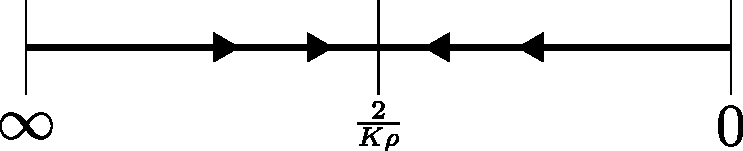
\includegraphics[width=0.4\textwidth]{rg_flow_pms.pdf}
	\caption{Attractive finite \(J\) fixed point of poor man scaling RG equation}
\end{figure}
For \(D\) not so large, the denominator also comes into play, and Eq.~\ref{mchannel} holds. We get the possibility of two fixed points - one from the numerator and the other from the numerator.
\begin{figure}[!htb]
	\centering
	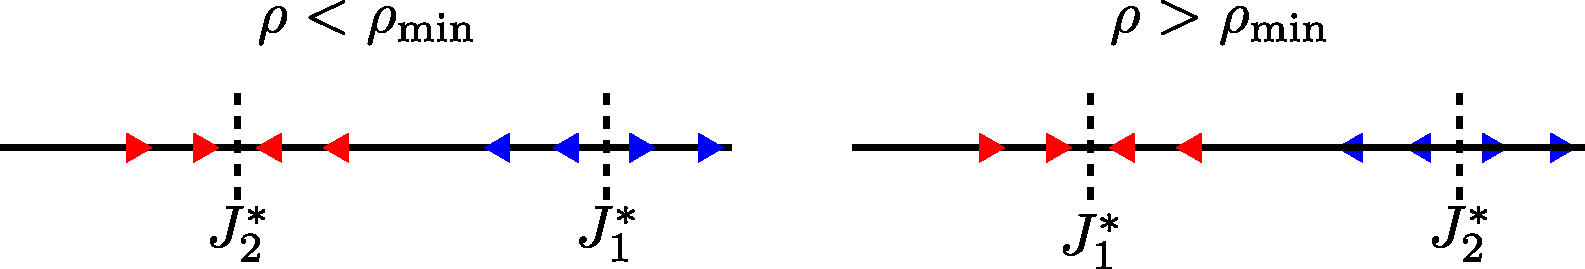
\includegraphics[width=0.7\textwidth]{./rg_flow.pdf}
	\caption{}
	\label{rg_flow_general}
\end{figure}

The numerator and denominator fixed points, \(J_1^*\) and \(J_2^*\) respectively, are given by
\begin{align}
	J_1^* = \frac{2}{K \rho}, && D^* = \frac{J_2^*}{4}
\end{align}
For a given \(K\), the position of \(J_1^*\) will be governed by \(\rho\). In general, for each bare bandwidth \(D_0\), there exists a minimal \(\rho\), $\rho_\text{min}(D_0)$, above which the the lower fixed point is the one from the numerator. That is, for \(\rho > \rho_\text{min}\), if we start scaling from small \(J_0\), it grows until it hits \(J_1^*\) which acts as the attractive fixed point, and \(J_2^*\) lies at a higher value and acts as the repulsive fixed point. For \(\rho < \rho_\text{min}\), \(J\) will grow and hit \(J_2^*\) instead, and \(J_1^* > J_2^*\) now becomes the repulsive fixed point.
\begin{align}
	\rho_\text{min} = \text{minimum }\left\{\rho, \text{ such that } \frac{2}{K \rho} < 4 D^*(\rho)\right\}
\end{align}
The RG flows towards the attractive fixed point \(J_1^*\) is shown  in fig.~\ref{rg_flow_K-2}.
\begin{figure}[!htpb]
	\centering
	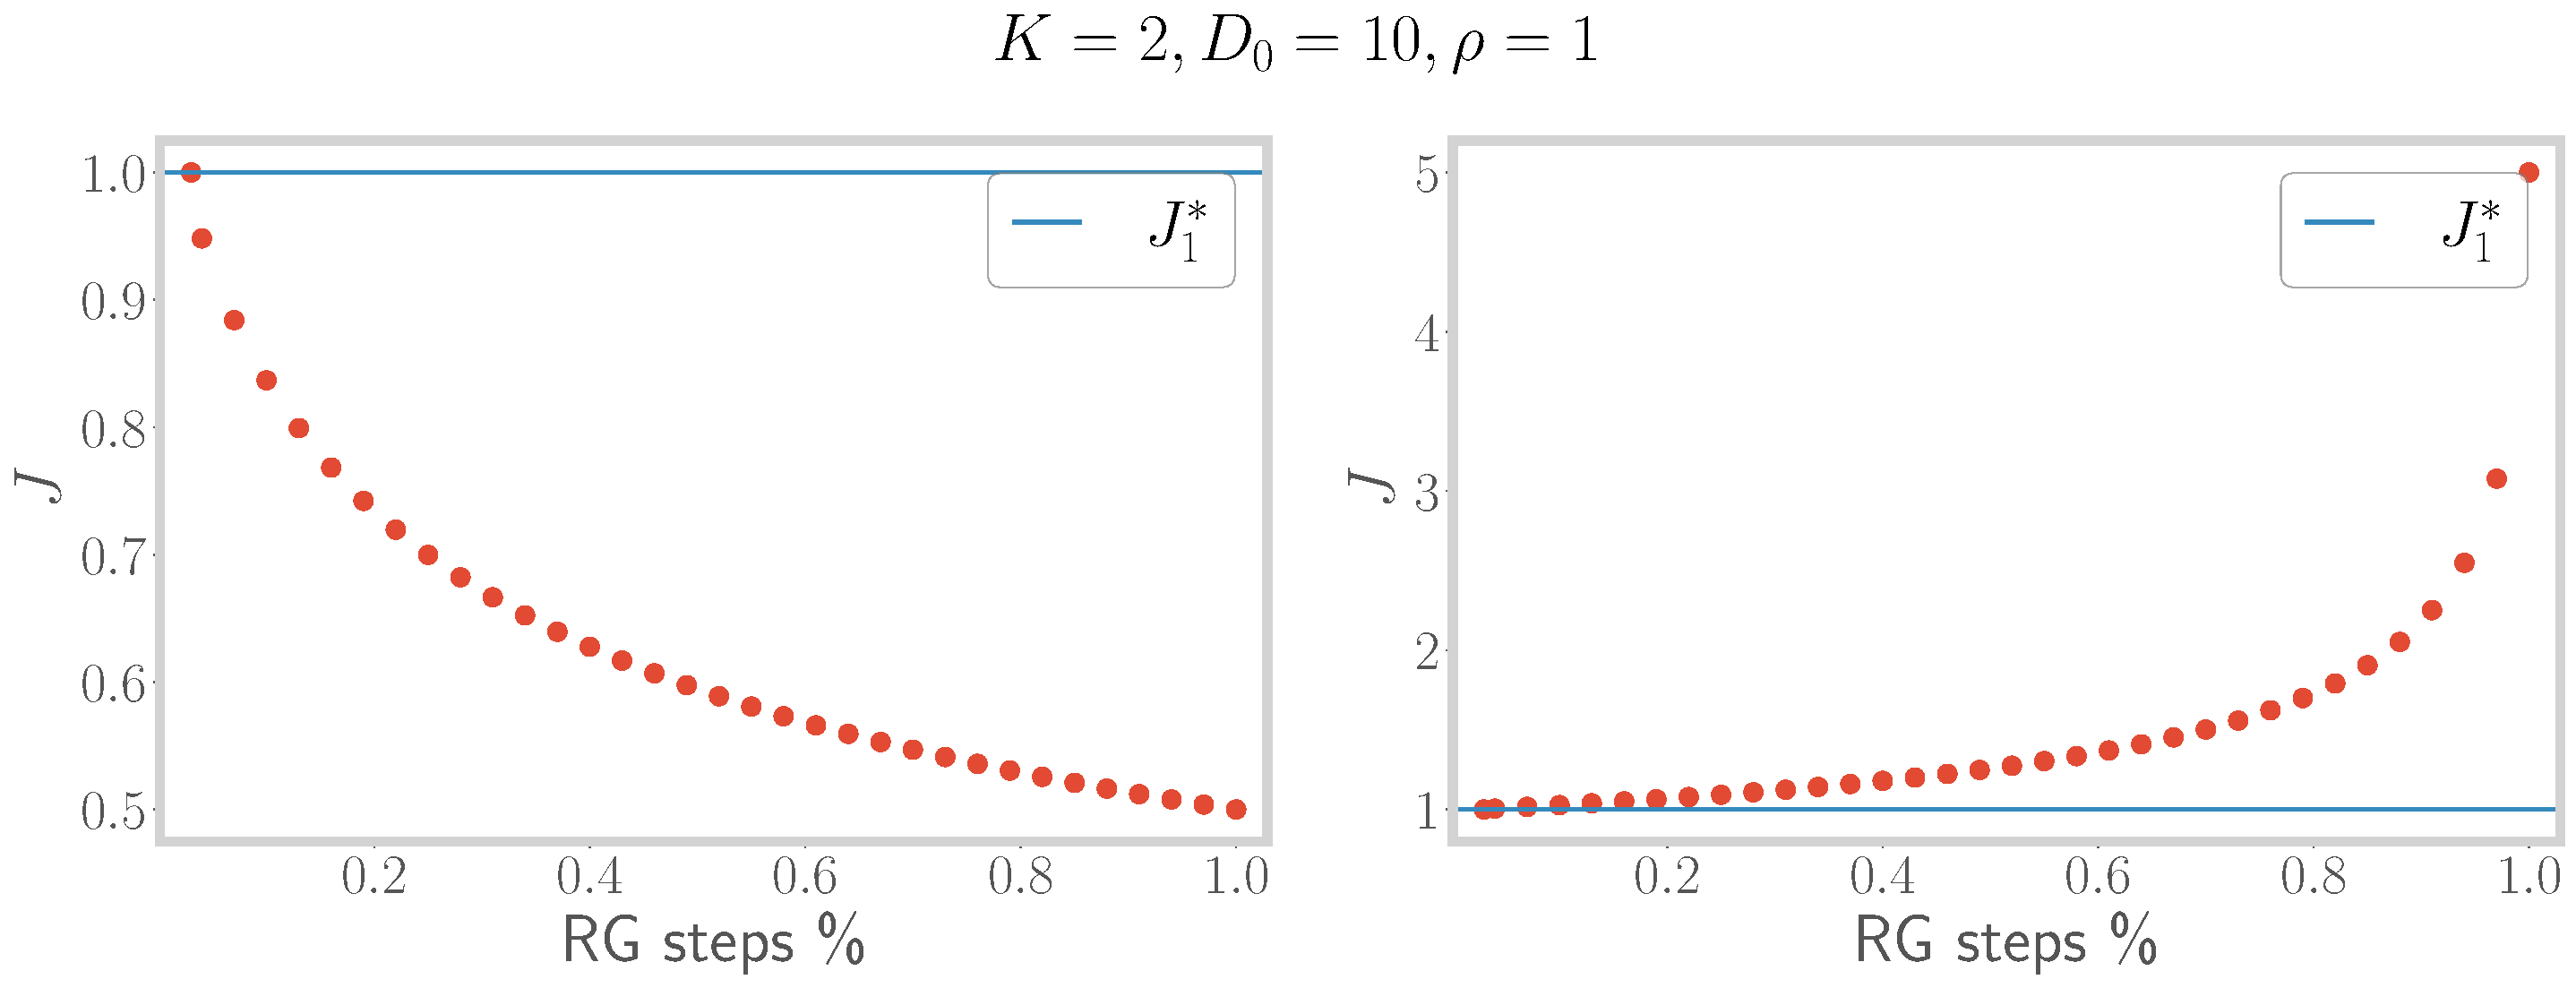
\includegraphics[width=0.8\textwidth]{../numerics/rg_flow_K=2.pdf}
	\caption{Flow of \(J\) towards the attractive fixed point \(J_1^*\), both from \(J<J_1^*\) (left panel) as well as from \(J>J_1^*\) (right panel).}
	\label{rg_flow_K-2}
\end{figure}

This behaviour is shown schematically in fig.~\ref{rg_flow_general}. 
\begin{figure}[!htb]
	\centering
	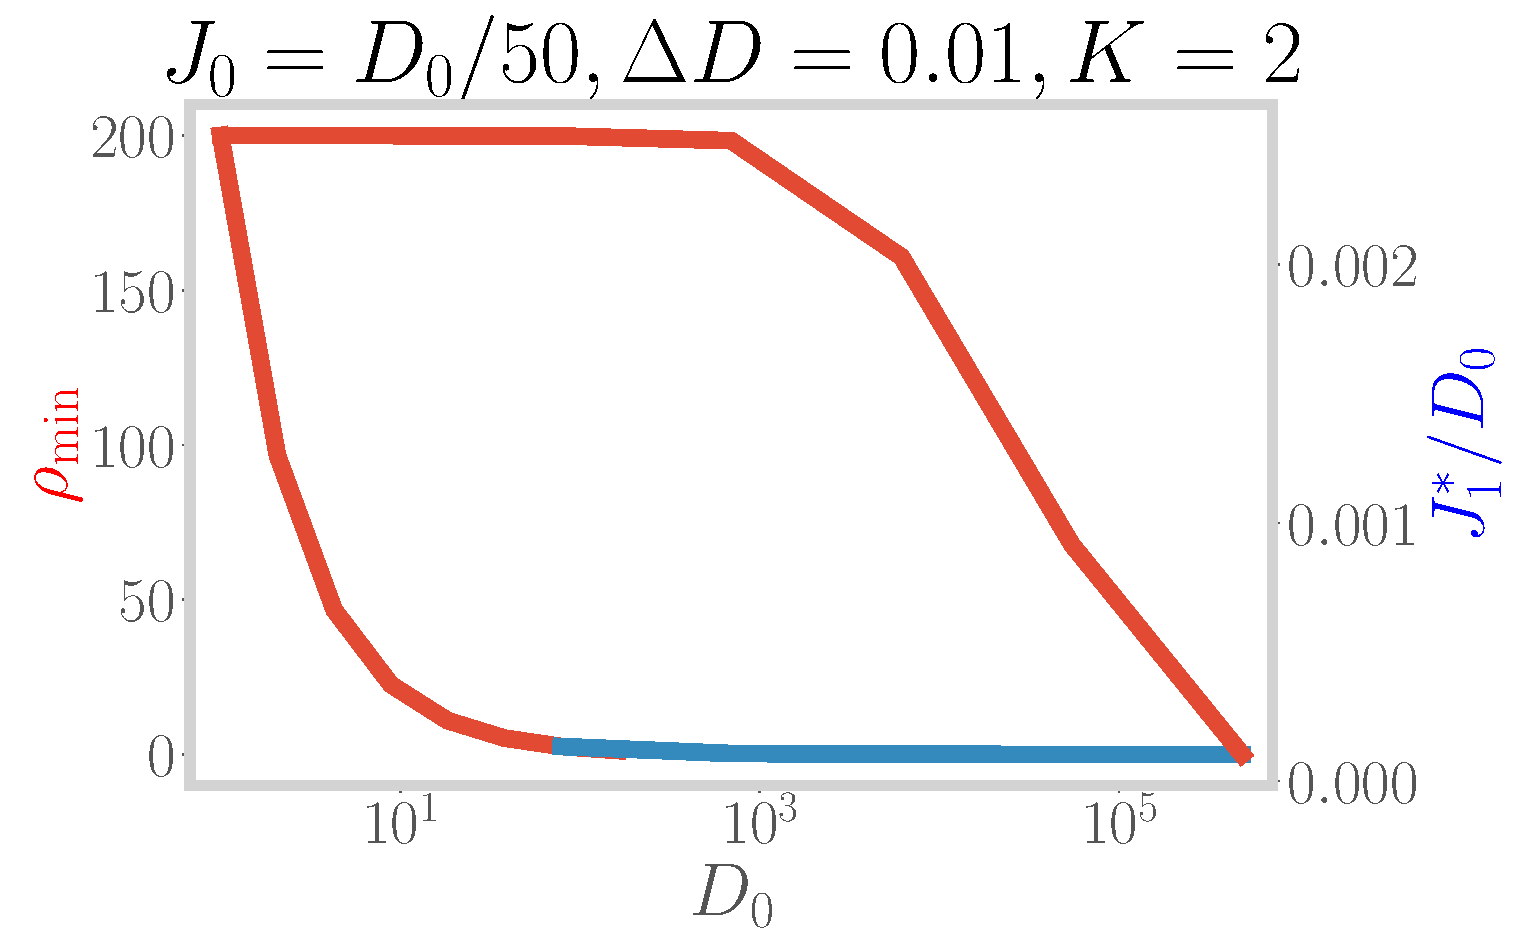
\includegraphics[width=0.5\textwidth]{../numerics/rhomin_D.pdf}
	\caption{Red curve shows variation of \(\rho_\text{min}\) against \(D_0\). It vanishes at large \(D_0\). Blue curve shows variation of the ratio \(J_1^* / D_0\) with \(D_0\). That shrinks as well, showing that the fixed point \(J_1^*\) remains finite in the thermodynamic limit, and the distance between \(J_1^*\) and \(J_2^*\) keeps growing.}
	\label{rhomin_vs_D}
\end{figure}
In fig.~\ref{rhomin_vs_D}, we plot \(\rho_\text{min}\) against the bare bandwidth. For large \(D_0\), it essentially shrinks to zero, and the numerator becomes the first fixed point for essentially all \(\rho\).

If we assume we are at a sufficiently large \(D_0\) and \(\rho > \rho_\text{min}\), the lower fixed point is \(J_1^*\). As shown in fig.~\ref{rhomin_vs_D}, we have \(J_1^* \ll D_0\). If we start with \(J_0\) in the neighborhood of \(J_1^*\), we can use \(J_1^* \ll D_0\) to ignore \(J\) in the denominator and the RG equation reduces to the poor man's scaling form Eq.~\ref{pms_mchannel}. The denominator fixed point has effectively moved off to infinity. That this is true can also be argued from the single-channel Kondo model URG results. There, we saw that when the bandwidth is scaled to larger values, the strong coupling fixed point was stable at successively larger values of \(J^*\). Since the denominator fixed point is identical in structure in both problems, its reasonable that the same thing will happen here.

\section{Effect of anisotropy on RG flows}
For a general anisotropic MCK, the Hamiltonian is
\begin{align}
	H = \sum_{k,\alpha,\gamma}\epsilon_{k}^\gamma \hat n^\gamma_{k\alpha} + \sum_{kk^\prime,\gamma}J_\gamma \vec{S_d}\cdot\vec{s}_{\alpha\alpha^\prime}{c^\gamma_{k\alpha}}^\dagger c^\gamma_{k^\prime\alpha^\prime}~.
\end{align}
Let us consider the specific case where \(K-1\) channels have the same coupling \(J_1 = J_2 = ... = J_{K-1} = J_+\) and the remaining channel has a different coupling \(J_K = J_-\). The RG equations for such a model are
\begin{align}
	\frac{\Delta J_+}{|\Delta D|} = \frac{J_+^2 \rho}{D - J_+/4} - \frac{\rho^2 J_+}{2}\left[\frac{(K-1)J_+^2}{D - J_+/4} + \frac{J_-^2}{D - J_-/4}\right]\\
	\frac{\Delta J_-}{|\Delta D|} = \frac{J_-^2 \rho}{D - J_-/4} - \frac{\rho^2 J_-}{2}\left[\frac{(K-1)J_+^2}{D - J_+/4} + \frac{J_-^2}{D - J_-/4}\right]
\end{align}
Setting \(J_+ = J_-\) leads to the critical fixed point at \(J_+^* = J_-^* = J_* = \frac{2}{K \rho}\). We now perturb around this fixed point by defining new variables \(j_\pm = J_\pm - J_*\). We also assume that \(D - J_\pm / 4 \simeq D - J_*/4\). The RG equations then take the form
\begin{align}
	\frac{\Delta j_+}{|\Delta D|} &= \frac{\rho J_+}{D - J_*/4}\left[J_+ - \frac{\rho}{2}\left[(K-1)J_+^2 + J_-^2\right]\right]\\
				      &= \frac{\rho J_+}{D - J_*/4}\left[j_+ + J_*- \frac{1}{K J_*}\left[(K-1)\left(J_* + j_+\right)^2 + \left(J_* + j_-\right)^2\right]\right]\\
				      &= \frac{\rho J_+}{K J_*\left(D - J_*/4\right)}\left[KJ_*\left(j_+ + J_*\right) - (K-1)\left(J_* + j_+\right)^2 - \left(J_* + j_-\right)^2\right]\\
				      &= \frac{\rho J_+}{K J_*\left(D - J_*/4\right)}\left[K\left(J_*j_+ + J_*^2\right) - (K-1)\left(J_*^2 + j_+^2 + 2J_* j_+\right) - \left(J_*^2 + j_-^2 + 2J_* j_-\right)\right]\\
				      &= \frac{\rho J_+}{K J_*\left(D - J_*/4\right)}\left[KJ_*j_+ - (K-1)\left(j_+^2 + 2J_* j_+\right) - \left(j_-^2 + 2J_* j_-\right)\right]\\
				      &= \frac{\rho J_+}{K J_*\left(D - J_*/4\right)}\left[-\left(K - 2\right)J_*j_+ - (K-1)j_+^2 - j_-^2 - 2J_* j_-\right]\\
	\frac{\Delta j_-}{|\Delta D|} &= \frac{J_- \rho}{D - J_*/4}\left[J_- - \frac{\rho}{2}\left[(K-1)J_+^2 + J_-^2\right]\right]\\
				      &= \frac{J_- \rho}{K J_*\left(D - J_*/4\right)}\left[K\left(J_*j_- + J_*^2\right) - (K-1)\left(J_*^2 + j_+^2 + 2J_* j_+\right) - \left(J_*^2 + j_-^2 + 2J_* j_-\right)\right]\\
				      &= \frac{J_- \rho}{K J_*\left(D - J_*/4\right)}\left[\left(K - 2\right)J_*j_-  - j_-^2 - (K-1)j_+^2 - 2(K-1)J_* j_+\right]\\
\end{align}
We will first look at the special case of \(K=2\), the two channel Kondo model. The equations simplify to
\begin{align}
	\frac{\Delta j_\pm}{|\Delta D|} = \frac{J_\pm \rho}{K J_*\left(D - J_*/4\right)}\left[- \left(j_+^2 + j_-^2\right) - 2J_* j_\mp\right]\\
\end{align}
For \(j_- < 0, j_+ > 0\), we have \(\Delta j_- < 0\). The coupling \(J_-\) therefore becomes irrelevant. For small \(j_+\), we have \(j_+^2 < 2J_* |j_-|\)  and \(\Delta j_+ > 0\). This means that the isotropic fixed point is repulsive under anisotropy~\cite{Noz_blandin_1980}. The coupling \(j_+\) being relevant means we have a single-channel Kondo problem. We already know the non-perturbative URG equation for the single-channel Kondo problem:
\begin{align}
	\frac{\Delta j_+}{|\Delta D|} = \frac{J_+^2 \rho}{D - J_+/4}~,
\end{align}
and it leads to the strong coupling fixed point

We now look at the general \(K\) channel case. Let us first look at the regime \(j_- < 0, j_+ > 0\). In this regime, we have \(\Delta j_- < 0\), which means \(j_-\) will flow to larger negative values until it reaches \(j_- = -J_*\) such that \(J_- = J_* + j_- = 0\). \(j_+\) is, on the other hand, relevant for small values of \(j_\pm\). It will continue to grow until the numerator of \(\Delta j_+\) vanishes. This condition is given by
\begin{align}
	\left(K - 2\right)J_*j_+ + (K-1)j_+^2 + j_-^2 + 2J_* j_- = 0
\end{align}
Substituting \(j_- = -J_*\) gives
\begin{align}
	(K-1)j_+^2 + \left(K - 2\right)J_*j_+ - J_*^2 = 0
\end{align}
Solving for \(j_+\) gives
\begin{align}
	j_{+,*} = \frac{-J_*(K-2) \pm \sqrt{(K-2)^2 J_*^2 + 4(K-1)J_*^2}}{2(K-1)} = \frac{J_*}{2(K-1)}\left[-(K-2) \pm K\right] = \frac{J_*}{K-1}
\end{align}
At the final step, we chose the positive solution, because \(j_+\) is relevant in this regime. The new fixed point value of \(J_+\) is therefore
\begin{align}
	J_{+,*} = J_* + \frac{J_*}{K-1} = \frac{\frac{2}{K \rho} K}{K - 1} = \frac{2}{(K-1)\rho}
\end{align}
In other words, the \(K\) channel fixed point flows to the \(K-1\) channel fixed point. This is shown numerically in fig.~\ref{K_to_K-1}.

\begin{figure}[htpb]
	\centering
	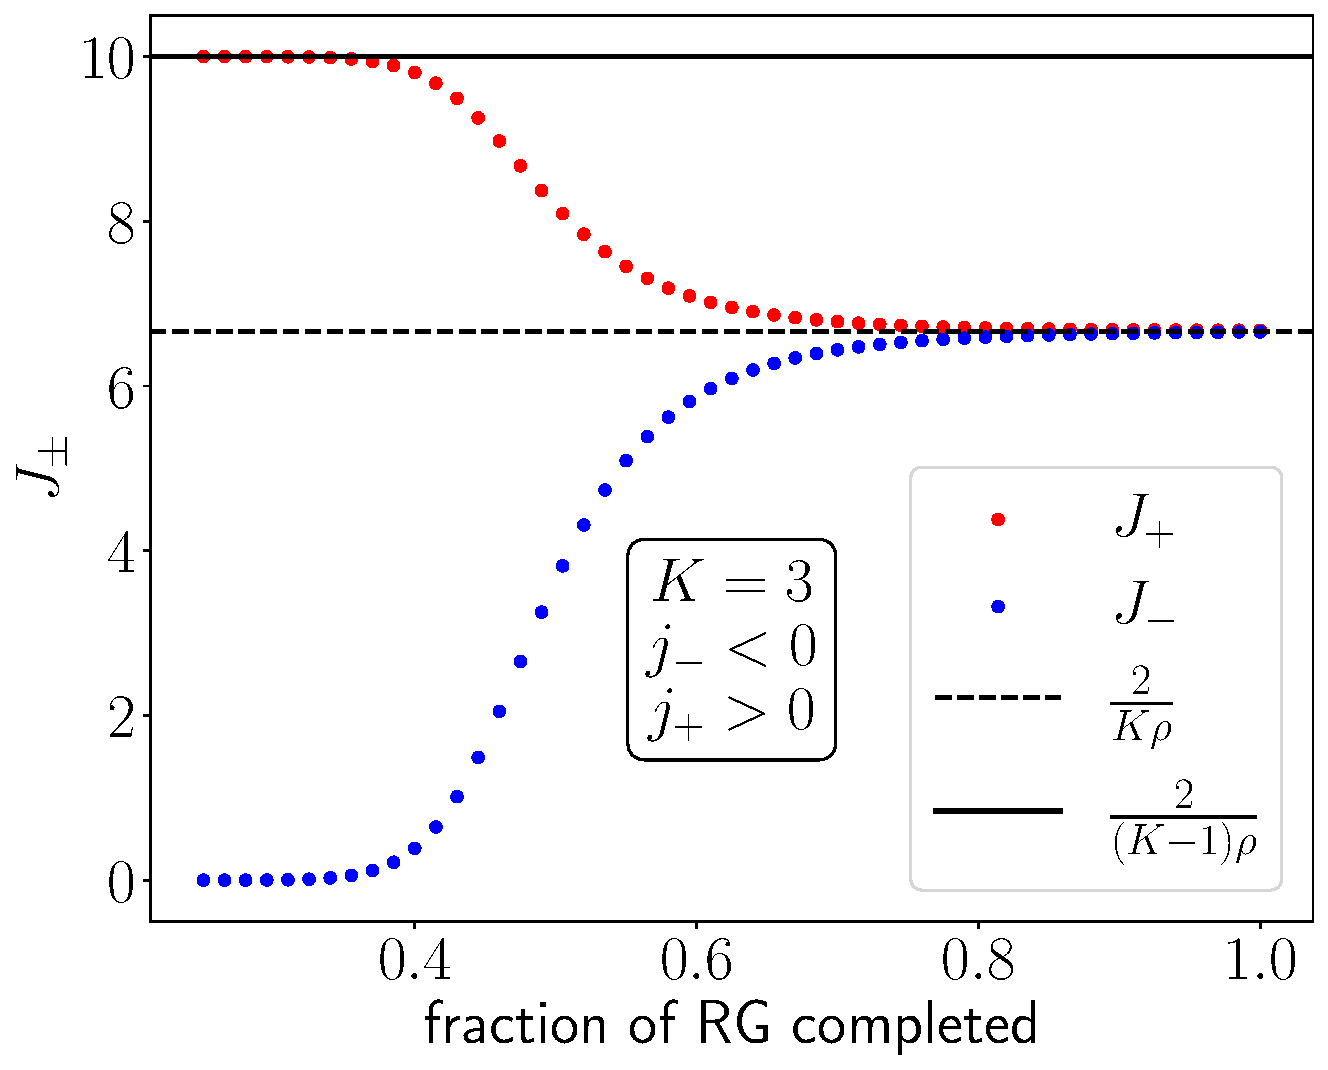
\includegraphics[width=0.4\textwidth]{../numerics/K to K-1.pdf}
	\caption{Flow of \(J_-\) to zero when \(j_< 0\) and \(J_+\) to the fixed point of the \(K-1\) channel Kondo model.}
	\label{K_to_K-1}
\end{figure}

In the opposite regime \(j_- > 0, j_+ < 0\), \(\Delta j_+\) is negative. It has been checked numerically that \(J_+\) ultimately flows to zero in this regime (fig. \ref{irrel_Jplus}), and \(J_-\) remains relevant. Since there is no numerator fixed point in the relevant coupling \(J_-\) and because all other couplings are irrelevant, the equation for \(J_-\) is replaced by the single-channel Kondo coupling URG equation, and the low-energy physics is then of strong coupling..
\begin{figure}[htpb]
	\centering
	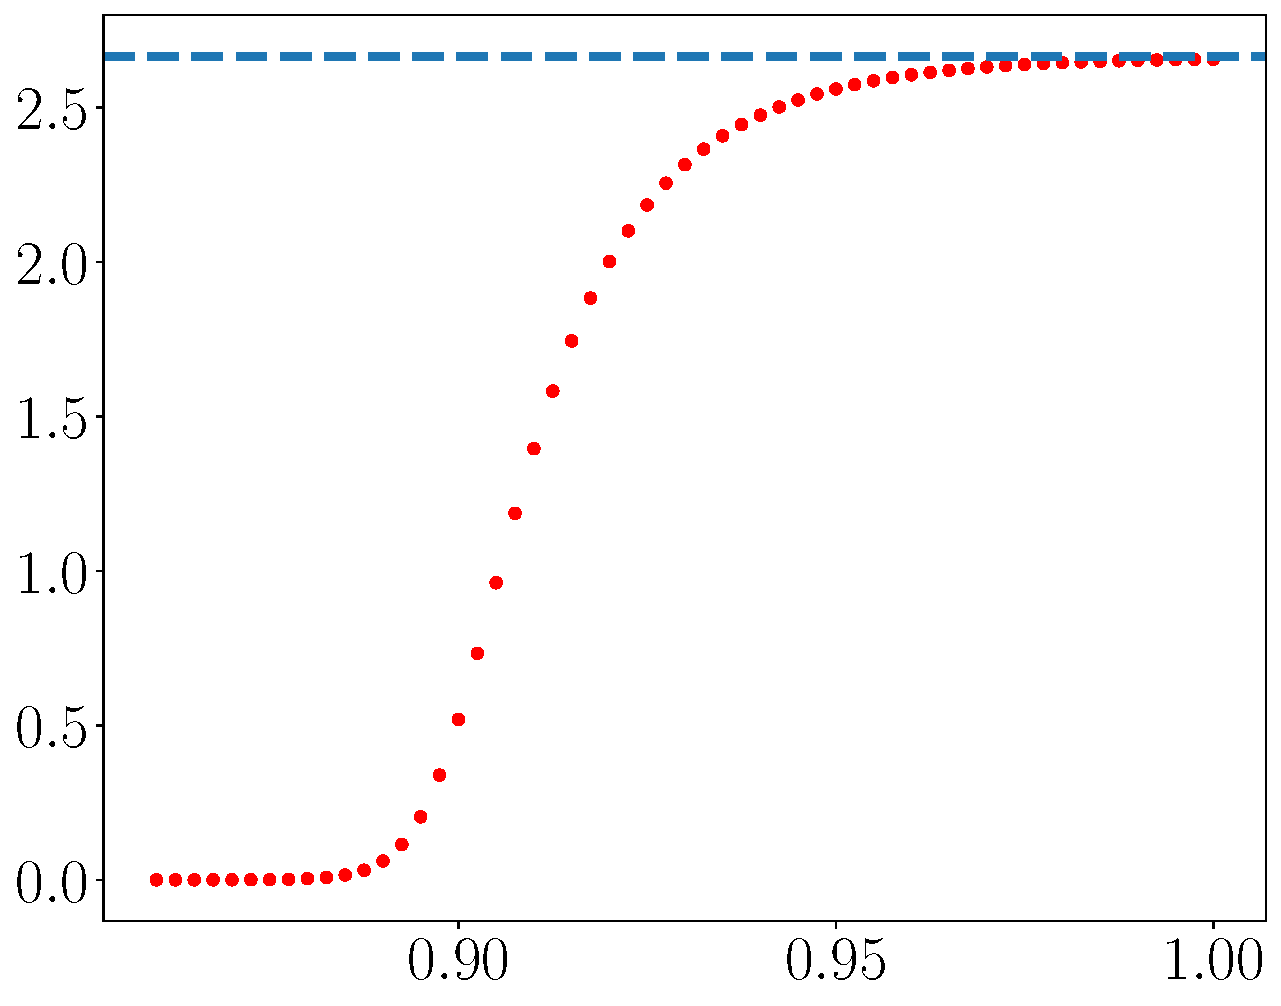
\includegraphics[width=0.45\textwidth]{../numerics/irr_Jp_K=3.pdf}
	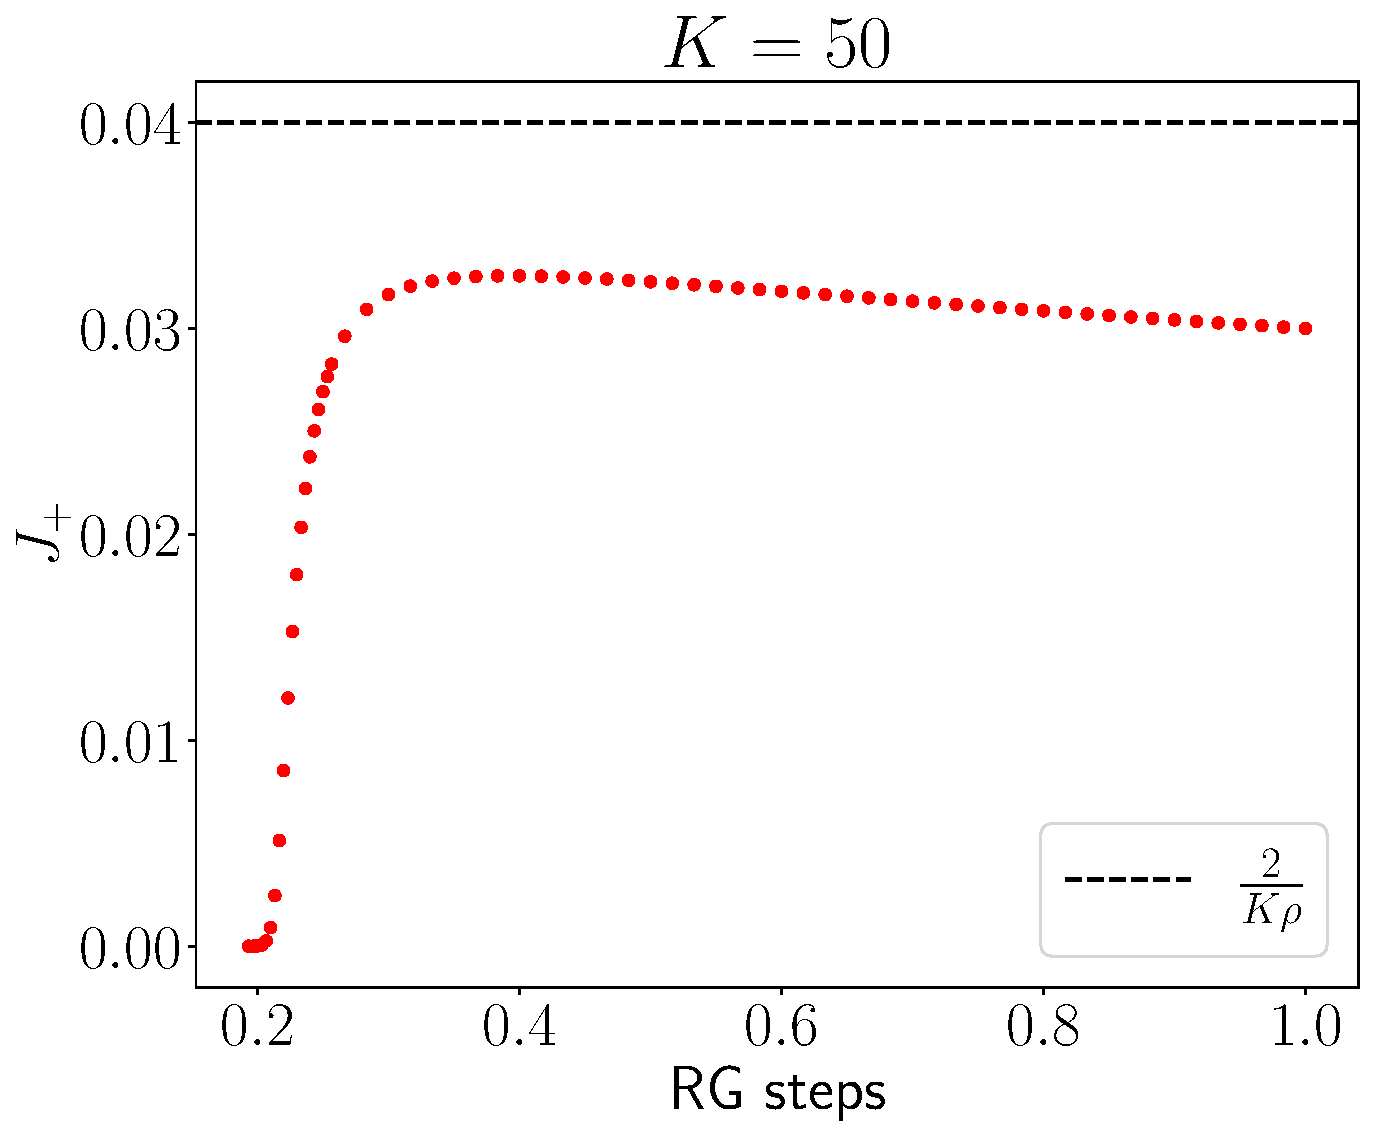
\includegraphics[width=0.45\textwidth]{../numerics/irr_Jp_K=50.pdf}
	\caption{Flow of the couplings \(J_+\) when \(j_+ < 0\) when \(j_- > 0, j_+ < 0\), for two values of \(K\).}
	\label{irrel_Jplus}
\end{figure}

\section{URG equations for the overscreened spin-\(S\) multi-channel Kondo model}
The leading order renormalization is the same as the single-channel model, and is shown in the appendix. Following that calculation, the Hamiltonian we will work with is 
\begin{equation}\begin{aligned}
	\label{H_spin_S}
    H = \sum_{k\sigma}\epsilon_{k}\tau_{k\sigma} + \sum_{m=-S}^S \sum_{kl,\atop{\sigma=\uparrow,\downarrow}} J^\sigma_m \ket{m}\bra{m} c^\dagger_{k \sigma}c_{l \sigma} + \sum_{kl} \sum_{m=-S}^{S-1} J^t_{m} \left(\ket{m+1}\bra{m} s^-_{kl}  + \text{h.c.}\right)
\end{aligned}\end{equation}
where \(\left\{\ket{m}\right\} \) are the eigenstates of \(S_d^z\), \(J^\sigma_m = \frac{1}{2} \sigma m J\) in the UV Hamiltonian, and \(J^t_{m} = J\frac{1}{2}\sqrt{S(S+1) - m(m+1)}\) is the coupling that connects \(\ket{m}\) and \(\ket{m+1}\). 

Following eq.~\ref{3rd_oder_terms}, the next order renormalization is of the form
\begin{equation}\begin{aligned}
	\Delta H^{(3)}_j = \underbrace{c^\dagger T \frac{1}{\omega^\prime - H_D} H_X \frac{1}{\omega^\prime - H_D} T^\dagger c + c^\dagger T \frac{1}{\omega^\prime - H_D} T^\dagger c \frac{1}{\omega^\prime - H_D} H_X}_\text{particle sector}\nonumber\\
	+ \underbrace{T^\dagger c \frac{1}{\omega - H_D} H_X \frac{1}{\omega - H_D} c^\dagger T + T^\dagger c \frac{1}{\omega - H_D} c^\dagger T \frac{1}{\omega - H_D} H_X}_\text{hole sector}
\end{aligned}\end{equation}

Because of eq.~\ref{H_spin_S}, the first term of the particle sector will be of the form
\begin{equation}\begin{aligned}
	\sum_{q,k,l_1} c^\dagger_{q\beta, l_1}c_{k \alpha, l_1}\ket{m_1}\bra{m_2} \frac{1}{\omega - \frac{D}{2} - \frac{\epsilon_k}{2} + \frac{\beta J}{4}S_d^z} \ket{m_2} c^\dagger_{k_1 \sigma_1, l_2}c_{k_2 \sigma_2,l_2} \bra{m_3}\frac{1}{\omega - \frac{D}{2} - \frac{\epsilon_k}{2} + \frac{\beta J}{4}S_d^z}\ket{m_3}\bra{m_4}c^\dagger_{k\alpha, l_1}c_{q\beta, l_1}
\end{aligned}\end{equation}
We have not bothered to write all the summations and the couplings correctly, because we will only simplify the denominator here. Evaluating the inner products gives
\begin{equation}\begin{aligned}
	\ket{m_1}\bra{m_4}\sum_k c^\dagger_{q\beta}c_{k \alpha} \frac{1}{\omega_{m_2,\beta} - \frac{D}{2} - \frac{\epsilon_k}{2} + \frac{\beta J m_2}{4}}  c^\dagger_{k_1 \sigma_1, l_2}c_{k_2 \sigma_2,l_2} \frac{1}{\omega_{m_3,\beta} - \frac{D}{2} - \frac{\epsilon_k}{2} + \frac{\beta J m_3}{4}}c^\dagger_{k\alpha}c_{q\beta}
\end{aligned}\end{equation}
To compare with the spin-\(\frac{1}{2}\) RG equations, we will transform the general spin-\(S\) \(\omega\) to the spin-\(\frac{1}{2}\) \( \omega\), using \(\omega_{m,\sigma} \to \omega - \frac{J}{2}\left(m\sigma - \frac{1}{2}\right)\).
\begin{equation}\begin{aligned}
	\hat n_{q\beta}\ket{m_1}\bra{m_4}c^\dagger_{k_1 \sigma_1, l_2}c_{k_2 \sigma_2,l_2}\sum_k \left( 1 - \hat n_{k\alpha} \right) \left(\frac{1}{\omega - \frac{D}{2} - \frac{\epsilon_k}{2} + \frac{J}{4}}\right)^2  
\end{aligned}\end{equation}
We can set \(\sum_q \hat n_{q\beta} = n(D)\). Performing the sums over \(k\) and \(l_1\) in the same fashion as previously gives
\begin{equation}\begin{aligned}
	-\frac{1}{2}\ket{m_1}\bra{m_4}c^\dagger_{k_1 \sigma_1, l_2}c_{k_2 \sigma_2,l_2} \frac{\rho n(D) K}{\omega - \frac{D}{2} + \frac{J}{4}}
\end{aligned}\end{equation}
Reinstating the complete summation and the couplings gives
\begin{equation}\begin{aligned}
	-\frac{1}{2}\frac{\rho n(D) K}{\omega - \frac{D}{2} + \frac{J}{4}}\sum_{m_1,m_4}\sum_{k_1,k_2,l_2,\sigma_1\sigma_2}\lambda_{1}\lambda_{2}\lambda_{3}\ket{m_1}\bra{m_4}c^\dagger_{k_1 \sigma_1, l_2}c_{k_2 \sigma_2,l_2}
\end{aligned}\end{equation}
There is no sum over \(m_2\) and \(m_3\) because they are constrained by \(m_1\) and \(m_4\) respectively. \(\lambda_i\) represent the couplings present at the three interaction vertices.

Similarly, using arguments identical to those used in the spin-\(\frac{1}{2}\) URG derivation (eq.~\ref{term2_sum}), the second term in the particle sector takes the form
\begin{equation}\begin{aligned}
	\frac{1}{2}\frac{\rho n(D) K}{\omega - \frac{D}{2} + \frac{J}{4}}\sum_{m_1,m_4}\sum_{k_1,k_2,l_2,\sigma_1\sigma_2}\lambda_{1}\lambda_{3}\lambda_{2}\ket{m_1}\bra{m_4}c^\dagger_{k_1 \sigma_1, l_2}c_{k_2 \sigma_2,l_2}
\end{aligned}\end{equation}

The first group of terms in the particle sector can be represented as \(a|b^\prime|c\), where \(a,b,c \in \left\{z,+,-\right\} \) and represent the operator for the conduction electrons in the three stages. The \(\prime\) on \(b\) indicates that it is the state of the electrons \textit{not being decoupled}. The second group of terms are therefore represented as \(a|b|c^\prime\), because in this group, the interaction \(H_X\) between the electrons not being decoupled occur at the very end.

We will only calculate the terms in the particle sector, the ones in hole sector will be equal to these because of particle-hole symmetry.
\paragraph{\(z|z^\prime|z\)}
\begin{equation}\begin{aligned}
	- \frac{1}{2}\frac{\rho n(D) K}{\omega - \frac{D}{2} + \frac{J}{4}}\sum_\beta \sum_{m}\sum_{k_1,k_2,l_2,\sigma} \left(J^\beta_m\right)^2 J^\sigma_m \ket{m}\bra{m}c^\dagger_{k_1 \sigma, l_2}c_{k_2 \sigma,l_2}
\end{aligned}\end{equation}

\paragraph{\(z|z|z^\prime\)}
\begin{equation}\begin{aligned}
	\frac{1}{2}\frac{\rho n(D) K}{\omega - \frac{D}{2} + \frac{J}{4}}\sum_\beta \sum_{m}\sum_{k_1,k_2,l_2,\sigma} \left(J^\beta_m\right)^2 J^\sigma_m \ket{m}\bra{m}c^\dagger_{k_1 \sigma, l_2}c_{k_2 \sigma,l_2}
\end{aligned}\end{equation}

\paragraph{\(-|z^\prime|+\)}
\begin{equation}\begin{aligned}
	-\frac{1}{2}\frac{\rho n(D) K}{\omega - \frac{D}{2} + \frac{J}{4}}\sum_{m}\sum_{k_1,k_2,l_2,\sigma} \left( J^t_m \right) ^2 J^\sigma_m \ket{m+1}\bra{m+1}c^\dagger_{k_1 \sigma, l_2}c_{k_2 \sigma,l_2}
\end{aligned}\end{equation}

\paragraph{\(-|+|z^\prime\)}
\begin{equation}\begin{aligned}
	\frac{1}{2}\frac{\rho n(D) K}{\omega - \frac{D}{2} + \frac{J}{4}}\sum_{m}\sum_{k_1,k_2,l_2,\sigma} \left( J^t_m \right) ^2 J^\sigma_{m+1} \ket{m+1}\bra{m+1}c^\dagger_{k_1 \sigma, l_2}c_{k_2 \sigma,l_2}
\end{aligned}\end{equation}

\paragraph{\(+|z^\prime|-\)}
\begin{equation}\begin{aligned}
	-\frac{1}{2}\frac{\rho n(D) K}{\omega - \frac{D}{2} + \frac{J}{4}}\sum_{m}\sum_{k_1,k_2,l_2,\sigma} \left( J^t_m \right) ^2 J^\sigma_{m+1} \ket{m}\bra{m}c^\dagger_{k_1 \sigma, l_2}c_{k_2 \sigma,l_2}
\end{aligned}\end{equation}

\paragraph{\(+|-|z^\prime\)}
\begin{equation}\begin{aligned}
	\frac{1}{2}\frac{\rho n(D) K}{\omega - \frac{D}{2} + \frac{J}{4}}\sum_{m}\sum_{k_1,k_2,l_2,\sigma} \left( J^t_m \right) ^2 J^\sigma_{m} \ket{m}\bra{m}c^\dagger_{k_1 \sigma, l_2}c_{k_2 \sigma,l_2}
\end{aligned}\end{equation}

\paragraph{\(z|+^\prime|z\)}
\begin{equation}\begin{aligned}
	-\frac{1}{2}\frac{\rho n(D) K}{\omega - \frac{D}{2} + \frac{J}{4}}\sum_\beta \sum_{m}\sum_{k_1,k_2,l_2}J^\beta_m J^t_m J^\beta_{m+1}\ket{m}\bra{m+1}c^\dagger_{k_1 \uparrow, l_2}c_{k_2 \downarrow,l_2}
\end{aligned}\end{equation}

\paragraph{\(z|-^\prime|z\)}
\begin{equation}\begin{aligned}
	-\frac{1}{2}\frac{\rho n(D) K}{\omega - \frac{D}{2} + \frac{J}{4}}\sum_\beta \sum_{m}\sum_{k_1,k_2,l_2} J^\beta_{m+1} J^t_m J^\beta_m \ket{m+1}\bra{m}c^\dagger_{k_1 \downarrow, l_2}c_{k_2 \uparrow,l_2}
\end{aligned}\end{equation}

\paragraph{\(+|+^\prime|-\)}
\begin{equation}\begin{aligned}
	-\frac{1}{2}\frac{\rho n(D) K}{\omega - \frac{D}{2} + \frac{J}{4}}\sum_{m}\sum_{k_1,k_2,l_2} J^t_m \left( J^t_{m+1} \right)^2 \ket{m}\bra{m+1}c^\dagger_{k_1 \uparrow, l_2}c_{k_2 \downarrow,l_2}
\end{aligned}\end{equation}
\paragraph{\(+|-^\prime|-\)}
\begin{equation}\begin{aligned}
	-\frac{1}{2}\frac{\rho n(D) K}{\omega - \frac{D}{2} + \frac{J}{4}}\sum_{m}\sum_{k_1,k_2,l_2} J^t_m \left( J^t_{m+1} \right)^2 \ket{m+1}\bra{m}c^\dagger_{k_1 \downarrow, l_2}c_{k_2 \uparrow,l_2}
\end{aligned}\end{equation}
\paragraph{\(-|-^\prime|+\)}
\begin{equation}\begin{aligned}
	-\frac{1}{2}\frac{\rho n(D) K}{\omega - \frac{D}{2} + \frac{J}{4}}\sum_{m}\sum_{k_1,k_2,l_2} \left( J^t_{m} \right)^2 J^t_{m+1}\ket{m+2}\bra{m+1}c^\dagger_{k_1 \downarrow, l_2}c_{k_2 \uparrow,l_2}
\end{aligned}\end{equation}
\paragraph{\(-|+^\prime|+\)}
\begin{equation}\begin{aligned}
	-\frac{1}{2}\frac{\rho n(D) K}{\omega - \frac{D}{2} + \frac{J}{4}}\sum_{m}\sum_{k_1,k_2,l_2} \left( J^t_{m} \right)^2 J^t_{m+1}\ket{m+1}\bra{m+2}c^\dagger_{k_1 \uparrow, l_2}c_{k_2 \downarrow,l_2}
\end{aligned}\end{equation}

\paragraph{\(z|z|+^\prime\)}
\begin{equation}\begin{aligned}
	\frac{1}{2}\frac{\rho n(D) K}{\omega - \frac{D}{2} + \frac{J}{4}}\sum_\beta \sum_{m}\sum_{k_1,k_2,l_2}\left(J^\beta_m\right)^2 J^t_m \ket{m}\bra{m+1}c^\dagger_{k_1 \uparrow, l_2}c_{k_2 \downarrow,l_2}
\end{aligned}\end{equation}

\paragraph{\(z|z|-^\prime\)}
\begin{equation}\begin{aligned}
	\frac{1}{2}\frac{\rho n(D) K}{\omega - \frac{D}{2} + \frac{J}{4}}\sum_\beta \sum_{m}\sum_{k_1,k_2,l_2}\left(J^\beta_m\right)^2 J^t_m \ket{m+1}\bra{m} c^\dagger_{k_1 \uparrow, l_2}c_{k_2 \downarrow,l_2}
\end{aligned}\end{equation}

\paragraph{\(+|-|+^\prime\)}
\begin{equation}\begin{aligned}
	\frac{1}{2}\frac{\rho n(D) K}{\omega - \frac{D}{2} + \frac{J}{4}}\sum_{m}\sum_{k_1,k_2,l_2} \left( J^t_{m} \right)^3 \ket{m}\bra{m+1}c^\dagger_{k_1 \uparrow, l_2}c_{k_2 \downarrow,l_2}
\end{aligned}\end{equation}

\paragraph{\(+|-|-^\prime\)}
\begin{equation}\begin{aligned}
	\frac{1}{2}\frac{\rho n(D) K}{\omega - \frac{D}{2} + \frac{J}{4}}\sum_{m}\sum_{k_1,k_2,l_2} J^t_m \left( J^t_{m+1} \right)^2 \ket{m+1}\bra{m}c^\dagger_{k_1 \downarrow, l_2}c_{k_2 \uparrow,l_2}
\end{aligned}\end{equation}
\paragraph{\(-|+|-^\prime\)}
\begin{equation}\begin{aligned}
	\frac{1}{2}\frac{\rho n(D) K}{\omega - \frac{D}{2} + \frac{J}{4}}\sum_{m}\sum_{k_1,k_2,l_2} \left( J^t_{m} \right)^3\ket{m+1}\bra{m}c^\dagger_{k_1 \downarrow, l_2}c_{k_2 \uparrow,l_2}
\end{aligned}\end{equation}

\paragraph{\(-|+|+^\prime\)}
\begin{equation}\begin{aligned}
	\frac{1}{2}\frac{\rho n(D) K}{\omega - \frac{D}{2} + \frac{J}{4}}\sum_{m}\sum_{k_1,k_2,l_2} \left( J^t_{m} \right)^2 J^t_{m+1}\ket{m+1}\bra{m+2}c^\dagger_{k_1 \uparrow, l_2}c_{k_2 \downarrow,l_2}
\end{aligned}\end{equation}

The terms \(a,l\) and \(j\) cancel out \(b,r\) and \(p\) respectively. The terms \(b\) through \(f\) renormalize \(J^\sigma_m\):
\begin{equation}\begin{aligned}
	\Delta J^\sigma_m = \frac{1}{2}\frac{\rho n(D) K}{\omega - \frac{D}{2} + \frac{J}{4}}\left[\left( J^t_{m-1} \right)^2 J^\sigma_m + \left( J^t_m \right)^2 J^\sigma_m - \left( J^t_{m-1} \right)^2 J^\sigma_{m-1} - \left(J^t_m\right)^2 J^\sigma_{m+1} \right] = \frac{1}{2}\frac{\rho n(D) K}{\omega - \frac{D}{2} + \frac{J}{4}}J^3 m \sigma
\end{aligned}\end{equation}
Since we had defined \(J^\sigma_m \equiv \frac{1}{2}J m \sigma\), we have \(\Delta J = \frac{2}{m\sigma}\Delta J^\sigma_m\), and we get
\begin{equation}\begin{aligned}
	\Delta_\text{p sector} J = \frac{1}{4}\frac{\rho n(D) K}{\omega - \frac{D}{2} + \frac{J}{4}}J^3
\end{aligned}\end{equation}

Since we started with an \(SU(2S+1)\times SU(2K+1)\) symmetric model, we can recover the RG equation for \(J\) from the transverse part as well. The transverse coupling \(J^t_m\) is renormalized by the terms \(g,i,m\) and \(o\).
\begin{equation}\begin{aligned}
	\Delta J^t_m = \frac{1}{2}\frac{\rho n(D) K}{\omega - \frac{D}{2} + \frac{J}{4}}\left[J^t_m\sum_\beta J^\beta_m\left(J^\beta_m - J^\beta_{m+1}\right) + J^t_m \left\{ \left( J^t_m \right) ^2 - \left( J^t_{m+1} \right) ^2 \right\} \right] = \frac{1}{4}\frac{\rho n(D) K}{\omega - \frac{D}{2} + \frac{J}{4}} J^2 J^t_m
\end{aligned}\end{equation}
Using \(J^t_m \equiv J\lambda_m\), we have
\begin{equation}\begin{aligned}
	\Delta_\text{h sector} J = \frac{1}{4}\frac{\rho n(D) K}{\omega - \frac{D}{2} + \frac{J}{4}} J^3
\end{aligned}\end{equation}
which is the same as the one previously obtained from the Ising part. The conclusion therefore is that the renormalization in the Kondo coupling for the overscreened models is independent of the impurity spin multiplicity.

The hole sector gives an identical contribution to the RG equation, so that the total renormalization in the Kondo coupling for an overscreened spin-\(S\) impurity is
\begin{equation}\begin{aligned}
	\Delta J = \frac{1}{2}\frac{\rho n(D) K}{\omega - \frac{D}{2} + \frac{J}{4}} J^3
\end{aligned}\end{equation}

\section{RG flow of axis anisotropy term}
We now insert a symmetry-breaking term in the Hamiltonian and study the RG flow of this term:
\begin{equation}\begin{aligned}
	\mathcal{H} = \sum_{k\sigma}\epsilon_{k}\tau_{k\sigma} + \sum_{kl} J S_d^z s^z_{kl} + \frac{1}{2}\sum_{kl} J \left(S_d^+ s^-_{kl}  + S_d^- s^+_{kl}\right) + X \left(J^z\right)^2
\end{aligned}\end{equation}
Here, \(s^z_{kl} = \frac{1}{2}\left(c^\dagger_{k\uparrow}c_{l \uparrow} - c^\dagger_{k\downarrow}c_{l \downarrow}\right)\), \(s^-_{kl} = c^\dagger_{k \downarrow}c_{l \uparrow}\) and \(s^+_{kl} = {s^-_{lk}}^\dagger\). Also, \(\tau = \hat n - \frac{1}{2}\). The indices \(k,l\) sum over the momentum states. \(\vec S_d\) is the impurity spin operator with \(S_d^z = \pm \frac{1}{2}\). \(X\) is the symmetry-breaking coupling, and \(J^z = S_d^z + s^z_\text{tot}\) is the total spin. Using \(\left(J^z\right)^2 = \frac{1}{4} + 2S_d^z s^z_\text{tot} + \left(s^z_\text{tot}\right)^2 \), we can rewrite the Hamiltonian as
\begin{equation}\begin{aligned}
	\mathcal{H} = \sum_{k\sigma}\epsilon_{k}\tau_{k\sigma} + \sum_{kl} J_\parallel S_d^z s^z_{kl} + \frac{1}{2}\sum_{kl} J_\perp \left(S_d^+ s^-_{kl}  + S_d^- s^+_{kl}\right) + X \sum_{k_1,k_2,k_1^\prime,\atop{k_2^\prime,l_1,l_2,\atop{\sigma_1,\sigma_2}}}\frac{\sigma_1\sigma_2}{4} c^\dagger_{k_1\sigma_1,l_1}c_{k_1^\prime\sigma_1,l_1}c^\dagger_{k_2\sigma_2,l_2}c_{k_2^\prime\sigma_2,l_2}
\end{aligned}\end{equation}

The following terms renormalize \(X\):
\paragraph{\(+|-|z\)}
\paragraph{\(-|+|z\)}
\paragraph{\(+|z|-\)}
\paragraph{\(-|z|+\)}
\paragraph{\(z|+|-\)}
\paragraph{\(z|-|+\)}
\paragraph{\(z|z|X\)}
\paragraph{\(+|-|X\)}
\paragraph{\(-|+|X\)}





\section{Duality in the MCK model}
We start from a strong coupling \((J \to \infty)\) spin-\(S\) impurity MCK Hamiltonian in the over-screened regime \(\left( K > 2S \right) \),
\begin{equation}\begin{aligned}
	\label{strong_ham}
	H(J) = \sum_{k,\sigma,l}\epsilon_{k,l} \hat n_{k\sigma,l} + J \vec{S_d}\cdot\vec{s}_\text{tot}~.
\end{aligned}\end{equation}
Here, \(\vec s_\text{tot}\) is the total spin \(\sum_l \sum_{kk^\prime \alpha\beta} \vec \sigma_{\alpha\beta}c^\dagger_{k\alpha,l}c_{k^\prime\beta,l}\) of all the zero modes. At strong-coupling, the ground states of the star graph eq.~\ref{zeromode_ham} act as a good starting point for a perturbative expansion. As argued previously, there are \(K-2S+1\) ground states, labelled by the \(K\) values of the total spin angular momentum \(S^z = S_d^z + s_\text{tot}^z = -\frac{K}{2} + S, -\frac{K}{2} + S + 1, \ldots, \frac{K}{2} - S\). To leverage the large coupling, one can define a new spin impurity \(\mathbb{S}\) out of this ground state manifold. Since the degeneracy of a spin is given by its multiplicity \(2S^\prime + 1\), we have \(2S^\prime + 1 = K-2S+1 \implies S^\prime = \frac{K}{2} - S\). That is, the spin-\(S\) impurity has a dual described by a spin-\((K-2S+1)\) impurity. The states of this new spin are defined by
\begin{equation}\begin{aligned}
	\mathbb{S}_d^z \ket{S^z} = S^z \ket{S^z}, &&\mathbb{S}_d^\pm \ket{S^z} = \sqrt{S^\prime\left( S^\prime + 1 \right) - S^z\left( S^z \pm 1\right)} \ket{S^z \pm 1}
\end{aligned}\end{equation}
The excited states of the star graph can be used to define bosons \cite{kroha_kolf_2007}, and the hopping into the lattice can then be re-written using these bosons. One can then remove the single-particle hoping between the zero modes and the first sites using a Schrieffer-Wolff transformation in the small coupling \(J^\prime = \gamma \frac{4t^2}{J}\), and generate an exchange-coupling between the new impurity \(\vec {\mathbb{S}}_d\) and the new zero modes formed out of the remaining sites in the lattice \cite{kroha_kolf_2007} (by remaining, we mean those real space sites that have not been consumed into forming the new spin). The new Hamiltonian, characterised by the small superexchange  coupling \(J^\prime\), has the form
\begin{equation}\begin{aligned}
	H^\prime(J^\prime) = \sum_{k,\sigma,l}\epsilon_{k,l} \hat n_{k\sigma,l} + J^\prime \vec{\mathbb{S}_d}\cdot\vec{s^\prime}_\text{tot}
\end{aligned}\end{equation}
The prime on \(s_\text{tot}\) indicates that it is formed by the new zero modes. This Hamiltonian is very similar to the one in eq.~\ref{strong_ham}, and that is the essence of the strong-weak duality: One can go from the over-screened strong coupling spin-\(S\) MCK model to another over-screened weak coupling spin-\((K-2S+1)\) MCK model. For the case of \(K=4S\), we have \(S^\prime = S\), and both \(S_d\) and \(\mathbb{S}_d\) describe the same spin objects (at least formally). The two models are then said to be self-dual. For example, for the case of spin-half MCK model, two-channel model is self-dual.

One important consequence of the duality relationship between the two overscreened models is that the RG equations are also dual; while the strong coupling model has an irrelevant coupling \(J\) that flows down to the intermediate fixed point \(J^*\), the weak coupling model has a relevant coupling \(J^\prime\) that flows up to the same fixed point \({J^\prime}^* = J^*\). From the RG equation for the general spin-\(S\) MCK model, we know that \({J^\prime}^* = \frac{2}{K \rho^\prime}\), where \(\rho^\prime\) is the DOS for the bath of the weak coupling Hamiltonian. This constrains the form of the scaling factor \(\gamma\):
\begin{equation}\begin{aligned}
	{J^\prime}^* = \frac{\gamma 4t^2}{J^*} = \frac{2}{K \rho^\prime} \implies \gamma = \frac{1}{4t^2} {J^*}^2 = \frac{1}{K^2 t^2 \rho \rho^\prime}
\end{aligned}\end{equation}

There exists another set of dual points in the MCK model. This was hinted at when we looked at the degree of compassion in eq.~\ref{gamma}. Since \(\Gamma\) depends only on the magnitude of \(\delta\), both \(\pm \delta\) will give the same degree of compensation, same ground state energy and same ground state degeneracy \(\left(g^S_K = |\delta|+1\right)\). The definition of \(\delta\) gives the duality transformation as \(K \to 2S, S \to \frac{K}{2}\). That is, we transform from a \(K-\)channel MCK model with spin-\(S\) impurity, to a \(2S\)-channel MCK with a spin-\(\frac{K}{2}\) impurity. The exactly-screened model \(K=2S\) maps on to itself and is therefore self-dual under this transformation.

For \(K \neq 2S\), we transform an over-screened model into an under-screened model and vice versa. This duality relationship allows us to infer the RG scaling behaviour of one of the models if we know that of the other. If we know that for a certain pair of values \(K\) and \(S\), the \(K-\)channel MCK model with spin-\(S\) impurity has an intermediate fixed point, we can immediately conclude that the \(2S\)-channel spin-\(\frac{K}{2}\) model has a strong coupling fixed point.
\begin{figure}[htpb]
	\centering
	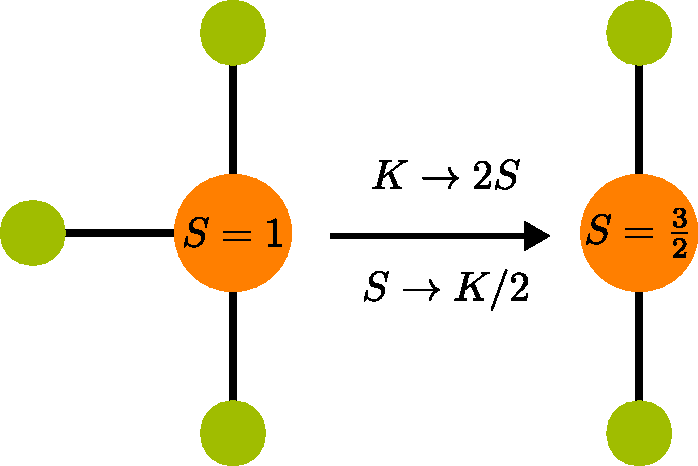
\includegraphics[width=0.45\textwidth]{./duality2.pdf}
	\caption{./duality2.pdf}
	\label{fig:-duality2-pdf}
\end{figure}

\subsection{Presence of a marginal Fermi liquid: Orthogonality catastrophe in two-channel MCK model}
At the stable fixed point \(J ^* = J_1^* = \frac{2}{K \rho}\), the ground states of the Hamiltonian are those of the star graph model, with a degeneracy of \(K\). We now specialise to the two-channel Kondo model. To find the low-energy excitations on top of this ground state manifold, we insert a tight-binding nearest-neighbour hopping between the zeroth site (the one that holds the impurity) and the first site (site that's nearest to the zeroth site) as a perturbation and calculate the diagonal and off-diagonal terms generated by this perturbation. It is found that when we trace out the impurity, we are left only with real space off-diagonal terms:
\begin{equation}\begin{aligned}
	\label{nfl_terms}
	V_\text{eff} = \frac{2t^2}{J^*}\left[\left(\sigma^z_{0,1}\right)^2 s^+_{0,2} + \left(\sigma^z_{0,2}\right)^2 s^+_{0,1}\right] \left(s^-_{1,1} + s^-_{1,2}\right) + \text{h.c.}
\end{aligned}\end{equation}
where \(\sigma^z_{0,l} = \hat n_{0\uparrow,l} - \hat n_{0\downarrow,l}, s^+ = c^\dagger_{0 \uparrow,l}c_{0 \downarrow,l}\) and \(s^- = \left(s^+\right)^\dagger\). The notation \(0\sigma,l\) has the site index \(i=0,1,2,\ldots\) as the first label, the spin index \(\sigma=\uparrow,\downarrow\) as the second label and the channel index \(l=1,2\) as the third index.

These are the terms that are generated because of the presence of the impurity. Such a non-Fermi liquid (NFL) contribution to the effective Hamiltonian and the absence of any Fermi-liquid term at the same order should be contrasted with the local Fermi liquid excitations induced by the singlet ground state of the single-channel Kondo model~\cite{nozieres1974fermi,wilson1975renormalization,hewson1993}. We wish to point out that such NFL terms were also obtained by Coleman, et al.~\cite{Coleman_tsvelik} in terms of Majorana fermions at the zeroth site and the first site of the \(\sigma-\tau\) version of the two-channel Kondo model. They then went on to compute a single-particle self-energy renormalisation coming from this NFL term that matches the phenomenological~\cite{varma2002singular} and microscopic forms of the marginal Fermi liquid self-energy~\cite{anirbanmott1,anirbanurg1}. We take a different route in order to calculate the self-energy contribution coming from Eq.~\ref{nfl_terms}.

In the URG analysis of the 2D Hubbard model at half-filling~\cite{anirbanurg1}, it was found that the normal phase of the Mott insulator was a metal with properties that have been phenomenologically attributed to the marginal Fermi liquid. The excitations of such a phase are described by a two particle-one hole composite object:
\begin{equation}\begin{aligned}
	\label{mfl_urg}
	H_\text{MFL} = \sum_{k,k^\prime,k^{\prime\prime},\sigma}R \hat n_{k\sigma} \hat n_{k^\prime \overline\sigma}\left(1 - \hat n_{k^{\prime\prime}\sigma}\right) 
\end{aligned}\end{equation}
We wish to look for such a term in the effective Hamiltonian. For this, we will perform a perturbative treatment of the hopping at strong coupling \(J \to \infty\) where the perturbative coupling \(t^2/J\) is arbitrarily small and again obtain Eq.~\ref{nfl_terms}. Such a change from the strong coupling model with parameter \(J\) to a weak coupling model with parameter \(t^2/J\) amounts to a duality transformation~\cite{kroha_kolf_2007,zitko_fabrizio_2017}. It can be shown that the duality transformation leads to an identical MCK model~\cite{kroha_kolf_2007} (self-duality), which implies we can have identical RG flows, and our transformation simply extracts the NFL piece from the dual model. The self-duality also ensures that the critical intermediate-coupling fixed point is unique and can be reached from either of the models.

The diagonal part of eq.~\ref{nfl_terms} is
\begin{equation}\begin{aligned}
	V_\text{eff} = \frac{2t^2}{J}\sum_{l=1,2}\left(\sum_\sigma \hat n_{0\sigma,l}\right) s^+_{0,\bar l}s^-_{1,\bar l} + \text{h.c.}
\end{aligned}\end{equation}
where \(\bar l = 3 - l\) is the channel index complementary to \(l\). We will fourier transform this effective Hamiltonian into \(k-\)space. The NFL part becomes
\begin{equation}\begin{aligned}
	\label{k_space_od}
	\sum_{\sigma, \left\{k_i,k_i^\prime\right\},l} \frac{2t^2}{J}e^{i\left(k_1 - k_1^\prime\right)a}c^\dagger_{k\sigma,l}c_{k^\prime\sigma,l}c^\dagger_{k_2 \uparrow, \bar l}c_{k_2^\prime \downarrow,\bar l}c^\dagger_{k_1 \downarrow,\bar l}c_{k_1^\prime \uparrow, \bar l} + \text{h.c.} 
\end{aligned}\end{equation}
This form of the Hamiltonian is very similar to the three-particle interaction term in Appendix B of~\cite{anirbanmott1}. The channel indices in Eq.~\ref{k_space_od} can be mapped to the normal directions in~\cite{anirbanmott1}. As specualted eariler, the 2 particle-1 hole interaction in Eq.~\ref{k_space_od} has a diagonal component which can be obtained by setting \(k=k^\prime, k_1 = k_2^\prime\) and \(k_2 = k_1^\prime\):
\begin{equation}\begin{aligned}
	H_\text{eff,MFL} = \sum_{k, k_1, \atop{k_2,\sigma,  l}} \frac{2t^2e^{i\left(k_1 - k_2\right)a}}{J} \hat n_{k\sigma,l} \hat n_{k_2 \uparrow, \bar l}\left(1 - \hat n_{k_1 \downarrow,\bar l}\right) + \text{h.c.}\\
	= \sum_{k, k_1, \atop{k_2,\sigma,  l}} \frac{4t^2}{J} \cos a\left(k_1 - k_2\right)  \hat n_{k\sigma,l} \hat n_{k_2 \uparrow, \bar l}\left(1 - \hat n_{k_1 \downarrow,\bar l}\right)
\end{aligned}\end{equation}
The most dominant contribution comes from \(k_1 = k_2 = k^\prime\), revealing the non-Fermi liquid metal~\cite{cox_jarrell_two_channel_rev,andrei_jerez_1995}:
\begin{equation}\begin{aligned}
	\label{mfl_large}
	H^*_\text{eff,MFL} = \frac{4t^2}{J} \sum_{\sigma, k, k^\prime, l} \hat n_{k\sigma,l} \hat n_{k^\prime \uparrow, \bar l}\left(1 - \hat n_{k^\prime \downarrow,\bar l}\right)
\end{aligned}\end{equation}
Following~\cite{anirbanmott1}, one can follow the RG evolution of the dual coupling \(R_j = \frac{4t^2}{J_j}\) at the \(j^\text{rh}\) RG step, in the form of the URG equation
\begin{equation}\begin{aligned}
	\Delta R_j =- \frac{R_j^2}{\omega - \epsilon_{j}/2 - R_j/8}
\end{aligned}\end{equation}
In the RG equation, \(\epsilon_{j}\) represents the energy of the \(j^\text{th}\) isoenergetic shell. It is seen from the RG equation that \(R\) is relevant in the range of \(\omega < \frac{1}{2}\epsilon_j\) that has been used throughout, leading to a fixed-point at \(R^*/8 = \omega - \frac{1}{2}\epsilon^*)\). The relevance of \(R\) is expected because the strong coupling \(J\) is irrelevant and \(R \sim 1/J\).

The renormalisation in \(R\) leads to a renormalisation in the single-particle self-energy~\cite{anirbanmott1}. The \(k-\)space-averaged self-energy renormalisation is
\begin{equation}\begin{aligned}
	\Delta \Sigma(\omega) = \rho {R^*}^2\int_0^{\epsilon^*} \frac{d\epsilon_j}{\omega - \epsilon_j/2 + R_j/8}
\end{aligned}\end{equation}
The density of states can be approximated to be \(N^*/R^*\), where \(N^*\) is the total number of states over the interval \(R^*\). As suggested by the fixed point value of \(R_j\), we can approximate its behaviour near the fixed point by a linear dependence of the dispersion \(\epsilon_j\). The two limits of the integration are the start and end points of the RG. We start the RG very close to the Fermi surface and move towards the fixed point \(\epsilon^*\). Near the start point, we substitute \(\epsilon = 0\) and \(R = \omega\), following the fixed point condition. From the the fixed point condition, we also substitute \(R^*/8 = \omega - \frac{1}{2}\epsilon^*\). On defining \(\bar \omega = N^* \left(\omega - \frac{1}{2}\epsilon^*\right)\), we can write
\begin{equation}\begin{aligned}
	\label{self_energy}
	\Delta \Sigma(\omega) \sim  \bar \omega \ln \frac{N^* \omega}{\bar \omega}
\end{aligned}\end{equation}
The self-energy also provides the quasiparticle residue for each channel\cite{anirbanmott1}:
\begin{equation}\begin{aligned}
	Z(\bar\omega) = \left(2 - \ln \frac{2\bar\omega}{N^* \omega}\right) ^{-1}
\end{aligned}\end{equation}
\textit{As the energy scale \(\omega \to 0\), the \(Z\) vanishes, implying that the ground state and lowest-lying excitations, in the presence of the NFL terms, are not adiabatically connected to the Fermi gas. This is the orthogonality catastrophe~\cite{varma2002singular,anderson_infraredcat,yamada_catastrophe,yamada1979orthogonality} in the two-channel Kondo problem, and it is brought about by the presence of the terms in Eq.~\ref{mfl_large}}. Such terms were absent in the single-channel Kondo model, because there was no multiply-degenerate ground state manifold that allowed scattering. This line of argument shows that the extra degeneracy of the ground state subspace and the frustration of the singlet order that comes about when one upgrades from the single-channel Kondo model to the MCK models is at the heart of the NFL behaviour, and the orthogonality catastrophe should be a general feature of all such frustrated MCK models. A local NFL term with a self-energy of the form in eq.~\ref{self_energy} was also obtained in the \(\sigma-\tau\) model by Coleman et al.~\cite{Coleman_tsvelik}. The common features show the universality between the two-channel Kondo and the \(\sigma-\tau\) models.

\section{Effective Hamiltonian for low-energy excitations: \(k-\)space}
The fixed point Hamiltonian is
\begin{align}
	H^* = H_0 + J^* \vec{S_d}\cdot\vec{s_\text{tot}}
\end{align}
where \(H_0 = \sum_{k,l,\sigma}\epsilon_{k,l}\hat n_{k\sigma,l}\) and \(\vec s_\text{tot} = \sum_l \vec s_l = \sum_{kk^\prime\alpha\alpha^\prime,l} \vec \sigma_{\alpha\alpha^\prime}c^\dagger_{k\alpha,l}c_{k^\prime\alpha^\prime,l}\). \(l\) sums over the channels. Henceforth we will drop the \(*\). Obtaining the effective Hamiltonian involves obtaining the low energy excitations on top of this fixed point Hamiltonian. The large-energy excitations are ones that involve spin flips. This guides the separation of the Hamiltonian into a diagonal and an off-diagonal piece:
\begin{align}
	H = H_d + V = \underbrace{H_0 + J S_d^z s_\text{tot}^z}_{H_d} + \underbrace{\frac{J}{2}S_d^+ s_\text{tot}^- + \text{h.c.}}_{V + V^\dagger}
\end{align}
We define \(V\) as the interaction term that decreases \(s_\text{tot}^z\) by 1: \(V \ket{s_\text{tot}^z} \to \ket{s_\text{tot}^z - 1}\). Similarly, we define \(V^\dagger \ket{s_\text{tot}^z} \to \ket{s_\text{tot}^z + 1}\). The effective Hamiltonian that has the states \(\ket{S_d^z, s_\text{tot}, s_\text{tot}^z}\) as eigenstates are
\begin{align}
	H_\text{eff} = H_d + V \frac{1}{E_\text{gs} - H_d}V = \sum_{k,l,\sigma}\epsilon_{k,l}\hat n_{k\sigma,l} + J S_d^z s_\text{tot}^z + \frac{J}{2}S_d^+ s_\text{tot}^- \frac{1}{E_\text{gs} - J S_d^z s_\text{tot}^z - H_0}\frac{J}{2}S_d^- s_\text{tot}^+\\
	+\frac{J}{2}S_d^- s_\text{tot}^+ \frac{1}{E_\text{gs} - J S_d^z s_\text{tot}^z - H_0}\frac{J}{2}S_d^+ s_\text{tot}^-
\end{align}
This is obtained from the Schrodinger equation for the ground state. If we expand the ground state in terms of \(\ket{S_d^z, s_\text{tot}, s_\text{tot}^z}\), we have 
\begin{align}
	\label{gstate_Expand}
\ket{\Psi_\text{gs}} = \sum_{S_d^z, s_\text{tot},s_\text{tot}^z}C_{S_d^z, s_\text{tot},s_\text{tot}^z}\ket{S_d^z, s_\text{tot}, s_\text{tot}^z}
\end{align}
The Schrodinger equation for the ground state can be written as
\begin{align}
	E_\text{gs}\ket{\Psi_\text{gs}} = H \ket{\Psi_\text{gs}} = \left(H_d + V\right)\ket{\Psi_\text{gs}} \implies \left(E_\text{gs} - H_d\right)\sum C_{S_d^z, s_\text{tot},s_\text{tot}^z}\ket{S_d^z, s_\text{tot}, s_\text{tot}^z} = V\sum C_{S_d^z, s_\text{tot},s_\text{tot}^z}\ket{S_d^z, s_\text{tot}, s_\text{tot}^z}
\end{align}
Since \(V\) only changes \(S_d^z \to -S_d^z\) and \(s^z_\text{tot} \to s^z_\text{tot} \pm 1\), we can simplify the equation into individual smaller equations. Let us take the case of two-channel, where the possible states are \(s_\text{tot},s^z_\text{tot} = (0,0), (1,-1), (1,0), (1,1)\). The individual equations for this model are
\begin{gather}
	\left(E_\text{gs} - H_d\right) \ket{S_d^z, 0, 0} = \left(E_\text{gs} - H_d\right) \ket{-\frac{1}{2}, 1, -1} = \left(E_\text{gs} - H_d\right) \ket{\frac{1}{2}, 1, 1}  = 0 \label{no_V}\\
	\left(E_\text{gs} - H_d\right) C_{\frac{1}{2}, 1, -1}\ket{\frac{1}{2}, 1, -1} = V C_{-\frac{1}{2}, 1, 0}\ket{-\frac{1}{2}, 1, 0}\label{eq2}\\
	\left(E_\text{gs} - H_d\right) C_{-\frac{1}{2}, 1, 0}\ket{-\frac{1}{2}, 1, 0} = V^\dagger C_{\frac{1}{2}, 1, -1}\ket{\frac{1}{2}, 1, -1}\label{eq3.2}\\
	\left(E_\text{gs} - H_d\right) C_{\frac{1}{2}, 1, 0}\ket{\frac{1}{2}, 1, 0} = V C_{-\frac{1}{2}, 1, 1}\ket{-\frac{1}{2}, 1, 1} \label{eq3.1}\\
	\left(E_\text{gs} - H_d\right) C_{-\frac{1}{2}, 1, 1}\ket{-\frac{1}{2}, 1, 1} = V^\dagger C_{\frac{1}{2}, 1, 0}\ket{\frac{1}{2}, 1, 0}\label{eq4}
\end{gather}
From eqs.~\ref{eq2} and \ref{eq4}, we can write
\begin{align}
	C_{\frac{1}{2}, 1, -1}\ket{\frac{1}{2}, 1, -1} &= C_{-\frac{1}{2}, 1, 0}\frac{1}{E_\text{gs} - H_d}V \ket{-\frac{1}{2}, 1, 0}, &&C_{-\frac{1}{2}, 1, 1}\ket{-\frac{1}{2}, 1, 1} = C_{\frac{1}{2}, 1, 0}\frac{1}{E_\text{gs} - H_d}V^\dagger \ket{\frac{1}{2}, 1, 0}
\end{align}
Substituting these into eqs.~\ref{eq3.1} and \ref{eq3.2} gives 
\begin{align}
	\label{eff_ham_Sdz_10}
	E_\text{gs} \ket{\frac{1}{2}, 1, 0} &= \left(H_d + V \frac{1}{E_\text{gs} - H_d}V^\dagger\right) \ket{\frac{1}{2}, 1, 0}\\
	E_\text{gs} \ket{-\frac{1}{2}, 1, 0} &= \left(H_d + V^\dagger \frac{1}{E_\text{gs} - H_d} V\right) \ket{-\frac{1}{2}, 1, 0}\\
\end{align}
These equations represent the Schrodinger equation for the states \(\ket{S_d^z, 1, 0}\), and the right hand sides therefore give the effective Hamiltonians for those states. If we combine the states into a single subspace \(\ket{1,0}= \left\{\ket{\frac{1}{2}, 1, 0}, \ket{-\frac{1}{2}, 1, 0}\right\}\), the effective Hamiltonian for this composite subspace becomes the sum of the two parts:
\begin{align}
	\label{eff_ham_10}
	H_\text{eff}\ket{1, 0}\bra{1, 0} = \left(H_d + V G_0 V^\dagger + V^\dagger G_0  V\right) \ket{1, 0}
\end{align}
where \(G_0 = \left(E_\text{gs} - H_d\right)^{-1}\). If we expand the subspace as \(\ket{1,0} = \ket{\frac{1}{2}, 1, 0} + \ket{-\frac{1}{2}, 1, 0}\), we recover eqs.~\ref{eff_ham_Sdz_10}. Solving similarly for the other states gives
\begin{align}
	H_\text{eff}\ket{1,  1}\bra{1,  1} &= \left(H_d + V^\dagger G_0  V\right) \ket{1,  1}\\
	H_\text{eff}\ket{1, - 1}\bra{1, - 1} &= \left(H_d + V G_0 V^\dagger\right) \ket{1, - 1}
\end{align}
\textit{One important conclusion that comes out of these calculations is that if the ground state is degenerate, the effective Hamiltonians is independent of which ground state we choose to start from in Eq.~\ref{gstate_Expand}. This is because the only difference in the various degenerate ground states is in the coefficients \(C_{S_d^z, s_\text{tot},s_\text{tot}^z}\). Since the final effective Hamiltonians are independent of these coefficients, they will be the same irrespective of which ground state we start with.}

To calculate these effective Hamiltonians, we will calculate the individual terms. We can easily simplify the \(S_d^z\) in the denominator of \(G_0\), because \(S_d^\pm \frac{1}{A + B S_d^z} = S_d^\pm \frac{1}{A \mp \frac{1}{2}B}\):
\begin{align}
	V G_0 V^\dagger = \frac{J^2}{4} s_\text{tot}^- \frac{\frac{1}{2} + S_d^z}{E_\text{gs} + \frac{J}{2} s_\text{tot}^z - H_0} s_\text{tot}^+ \\
	V^\dagger G_0 V = \frac{J^2}{4} s_\text{tot}^+ \frac{\frac{1}{2} - S_d^z}{E_\text{gs} - \frac{J}{2} s_\text{tot}^z - H_0} s_\text{tot}^-
\end{align}
Since \(H_0\) does not commute with the spin operators, we will need to expand the denominator to make sense of this Hamiltonian.
\begin{align}
	 V G_0 V^\dagger =  s_\text{tot}^- \frac{1}{E_\text{gs} + \frac{J}{2} s_\text{tot}^z}\left[1 + \frac{1}{E_\text{gs} + \frac{J}{2} s_\text{tot}^z}H_0 + \frac{1}{E_\text{gs} + \frac{J}{2} s_\text{tot}^z}H_0\frac{1}{E_\text{gs} + \frac{J}{2} s_\text{tot}^z}H_0 + \ldots\right] s_\text{tot}^+\\
	 V^\dagger G_0 V =  s_\text{tot}^+ \frac{1}{E_\text{gs} - \frac{J}{2} s_\text{tot}^z}\left[1 + \frac{1}{E_\text{gs} - \frac{J}{2} s_\text{tot}^z}H_0 + \frac{1}{E_\text{gs} - \frac{J}{2} s_\text{tot}^z}H_0\frac{1}{E_\text{gs} - \frac{J}{2} s_\text{tot}^z}H_0 + \ldots\right] s_\text{tot}^-
\end{align}
This is an expansion in \(H_0^n/J^{n+1}, n=0,1,2,\ldots\). The \(n=0\) terms give
\begin{align}
	s_\text{tot}^- \frac{1}{E_\text{gs} + \frac{J}{2} s_\text{tot}^z}s_\text{tot}^+ = s_\text{tot}^- s_\text{tot}^+ \frac{1}{E_\text{gs} + \frac{J}{2} \left(s_\text{tot}^z + 1\right)} %= \left[s_\text{tot}\left( s_\text{tot}+1 \right)  - s_\text{tot}^z\left( s_\text{tot}^z + 1 \right) \right] \frac{1}{E_\text{gs} + \frac{J}{2} \left(s_\text{tot}^z + 1\right)}\\ 
	\\
	s_\text{tot}^+ \frac{1}{E_\text{gs} - \frac{J}{2} s_\text{tot}^z}s_\text{tot}^- = s_\text{tot}^+ s_\text{tot}^- \frac{1}{E_\text{gs} - \frac{J}{2} \left(s_\text{tot}^z - 1\right)}% = \left[s_\text{tot}\left( s_\text{tot}+1 \right)  - s_\text{tot}^z\left( s_\text{tot}^z - 1 \right) \right] \frac{1}{E_\text{gs} - \frag{J}{2} \left(s_\text{tot}^z - 1\right)}
\end{align}

One of the \(n=1\) terms gives
\begin{align}
	s_\text{tot}^- \frac{1}{E_\text{gs} + \frac{J}{2} s_\text{tot}^z}\frac{1}{E_\text{gs} + \frac{J}{2} s_\text{tot}^z}H_0 s_\text{tot}^+ =  \left(\frac{1}{E_\text{gs} + \frac{J}{2} \left(s_\text{tot}^z + 1\right)}\right)^2 s_\text{tot}^- H_0 s_\text{tot}^+ 
\end{align}
Next we calculate the commutator:
\begin{align}
	\left[s_\text{tot}^+, H_0\right] = X^\dagger_{1,\text{tot}} = \sum_l X_{1,l}^\dagger = \sum_{kk^\prime,l}\left(\epsilon_k - \epsilon_{k^\prime}\right) c^\dagger_{k^\prime \uparrow} c_{k \downarrow}
\end{align}
where \(X_{n,l} \equiv \sum_{k,k^\prime}\left(\epsilon_k - \epsilon_{k^\prime}\right)^n c^\dagger_{k \downarrow}c_{k^\prime \uparrow} \).
Substituting this commutator gives
\begin{align}
	s_\text{tot}^- \frac{1}{E_\text{gs} + \frac{J}{2} s_\text{tot}^z}\frac{1}{E_\text{gs} + \frac{J}{2} s_\text{tot}^z}H_0 s_\text{tot}^+ =  \left(\frac{1}{E_\text{gs} + \frac{J}{2} \left(s_\text{tot}^z + 1\right)}\right)^2 \left(s_\text{tot}^- s_\text{tot}^+ H_0 - s_\text{tot}^- X^\dagger_{1,\text{tot}}\right)
\end{align}
The other \(n=1\) term gives
\begin{align}
	s_\text{tot}^+ \frac{1}{E_\text{gs} - \frac{J}{2} s_\text{tot}^z}\frac{1}{E_\text{gs} - \frac{J}{2} s_\text{tot}^z}H_0 s_\text{tot}^- =  \left(\frac{1}{E_\text{gs} - \frac{J}{2} \left(s_\text{tot}^z - 1\right)}\right)^2 \left(s_\text{tot}^+ s_\text{tot}^- H_0 + s_\text{tot}^+ X_{1,\text{tot}}\right)
\end{align}
One of the \(n=2\) terms gives
\begin{align}
	&s_\text{tot}^- \frac{1}{E_\text{gs} + \frac{J}{2} s_\text{tot}^z}\frac{1}{E_\text{gs} + \frac{J}{2} s_\text{tot}^z}H_0 \frac{1}{E_\text{gs} + \frac{J}{2} s_\text{tot}^z}H_0 s_\text{tot}^+\\
	&= \left(\frac{1}{E_\text{gs} + \frac{J}{2} \left(s_\text{tot}^z + 1\right)}\right)^2 s_\text{tot}^- H_0 \frac{1}{E_\text{gs} + \frac{J}{2} s_\text{tot}^z}H_0 s_\text{tot}^+ \\
	&= \left(\frac{1}{E_\text{gs} + \frac{J}{2} \left(s_\text{tot}^z + 1\right)}\right)^2 s_\text{tot}^- H_0 \frac{1}{E_\text{gs} + \frac{J}{2} s_\text{tot}^z}\left(s_\text{tot}^+ H_0 - X^\dagger_\text{1,tot}\right) \\
	&= \left(\frac{1}{E_\text{gs} + \frac{J}{2} \left(s_\text{tot}^z + 1\right)}\right)^2 \left[s_\text{tot}^- H_0 s_\text{tot}^+\frac{1}{E_\text{gs} + \frac{J}{2} \left(s_\text{tot}^z+1\right)} H_0 - s_\text{tot}^- H_0\frac{1}{E_\text{gs} + \frac{J}{2}s_\text{tot}^z}X^\dagger_\text{1,tot}\right] \\
	&= \left(\frac{1}{E_\text{gs} + \frac{J}{2} \left(s_\text{tot}^z + 1\right)}\right)^2 \left[s_\text{tot}^- \left(s_\text{tot}^+H_0 - X^\dagger_{1,\text{tot}}\right)\frac{1}{E_\text{gs} + \frac{J}{2} \left(s_\text{tot}^z+1\right)} H_0 - s_\text{tot}^- H_0\frac{1}{E_\text{gs} + \frac{J}{2}s_\text{tot}^z}X^\dagger_\text{1,tot}\right] \\
	&= \left(\frac{1}{E_\text{gs} + \frac{J}{2} \left(s_\text{tot}^z + 1\right)}\right)^2 \left[s_\text{tot}^- s_\text{tot}^+H_0\frac{1}{E_\text{gs} + \frac{J}{2} \left(s_\text{tot}^z+1\right)} H_0 - s_\text{tot}^-\left(X^\dagger_{1,\text{tot}}\frac{1}{E_\text{gs} + \frac{J}{2} \left(s_\text{tot}^z+1\right)} H_0 + H_0\frac{1}{E_\text{gs} + \frac{J}{2}s_\text{tot}^z}X^\dagger_\text{1,tot}\right)\right] \\
\end{align}
At this point, we need the commutator between \(H_0\) and \(s_\text{tot}^z\):
\begin{align}
	\left[H_0, s_\text{tot}^z\right] = Z_{1,\text{tot}} = \sum_l Z_{1, l} = \sum_{k,k^\prime,l}\left( \epsilon_k - \epsilon_{k^\prime} \right) \frac{1}{2}\left(c^\dagger_{k \uparrow,l}c_{k^\prime \uparrow,l} - c^\dagger_{k \downarrow,l}c_{k^\prime \downarrow,l}\right)
\end{align}
This gives the relation
\begin{align}
	H_0 (a + b s_\text{tot}^z) = (a + b s_\text{tot}^z) H_0 + Z_{1,\text{tot}} \implies \frac{1}{a + b s_\text{tot}^z} H_0 = H_0 \frac{1}{a + b s_\text{tot}^z} + \frac{1}{a + b s_\text{tot}^z} Z_{1,\text{tot}} \frac{1}{a + b s_\text{tot}^z}
\end{align}
Using this, we get
\begin{align}
	&s_\text{tot}^- \frac{1}{E_\text{gs} + \frac{J}{2} s_\text{tot}^z}\frac{1}{E_\text{gs} + \frac{J}{2} s_\text{tot}^z}H_0 \frac{1}{E_\text{gs} + \frac{J}{2} s_\text{tot}^z}H_0 s_\text{tot}^+\\
	&= \left(\frac{1}{E_\text{gs} + \frac{J}{2} \left(s_\text{tot}^z + 1\right)}\right)^2 \left[s_\text{tot}^- s_\text{tot}^+ \frac{1}{E_\text{gs} + \frac{J}{2} \left(s_\text{tot}^z+1\right)} H_0 H_0 - s_\text{tot}^- s_\text{tot}^+ \frac{1}{E_\text{gs} + \frac{J}{2} \left(s_\text{tot}^z+1\right)} Z_{1,\text{tot}} \frac{1}{E_\text{gs} + \frac{J}{2} \left(s_\text{tot}^z+1\right)}H_0\right.\\
	& \left.- s_\text{tot}^-\left(X^\dagger_{1,\text{tot}}\frac{1}{E_\text{gs} + \frac{J}{2} \left(s_\text{tot}^z+1\right)} H_0 + H_0\frac{1}{E_\text{gs} + \frac{J}{2}s_\text{tot}^z}X^\dagger_\text{1,tot}\right)\right] \\
	&= \left(\frac{1}{E_\text{gs} + \frac{J}{2} \left(s_\text{tot}^z + 1\right)}\right)^2 s_\text{tot}^- s_\text{tot}^+ \left[\frac{1}{E_\text{gs} + \frac{J}{2} \left(s_\text{tot}^z+1\right)} H_0 H_0 - \frac{1}{E_\text{gs} + \frac{J}{2} \left(s_\text{tot}^z+1\right)} Z_{1,\text{tot}} H_0\frac{1}{E_\text{gs} + \frac{J}{2} \left(s_\text{tot}^z+1\right)}\right]
\end{align}
At the last step, we dropped the three-particle scattering terms. 

The other \(n=2\) term gives
\begin{align}
	&s_\text{tot}^+ \frac{1}{E_\text{gs} - \frac{J}{2} s_\text{tot}^z}\frac{1}{E_\text{gs} - \frac{J}{2} s_\text{tot}^z}H_0 \frac{1}{E_\text{gs} - \frac{J}{2} s_\text{tot}^z}H_0 s_\text{tot}^-\\
	&= \left(\frac{1}{E_\text{gs} - \frac{J}{2} \left(s_\text{tot}^z - 1\right)}\right)^2 s_\text{tot}^+ H_0 \frac{1}{E_\text{gs} - \frac{J}{2} s_\text{tot}^z}H_0 s_\text{tot}^- \\
	&= \left(\frac{1}{E_\text{gs} - \frac{J}{2} \left(s_\text{tot}^z - 1\right)}\right)^2 s_\text{tot}^+ H_0 \frac{1}{E_\text{gs} - \frac{J}{2} s_\text{tot}^z}\left(s_\text{tot}^- H_0 + X_\text{1,tot}\right) \\
	&= \left(\frac{1}{E_\text{gs} - \frac{J}{2} \left(s_\text{tot}^z - 1\right)}\right)^2 \left[s_\text{tot}^+ H_0 s_\text{tot}^-\frac{1}{E_\text{gs} - \frac{J}{2} \left(s_\text{tot}^z - 1\right)} H_0 + s_\text{tot}^+ H_0\frac{1}{E_\text{gs} - \frac{J}{2}s_\text{tot}^z}X_\text{1,tot}\right] \\
	&= \left(\frac{1}{E_\text{gs} - \frac{J}{2} \left(s_\text{tot}^z - 1\right)}\right)^2 s_\text{tot}^+ \left(s_\text{tot}^- H_0 + X_\text{1,tot}\right)\frac{1}{E_\text{gs} - \frac{J}{2} \left(s_\text{tot}^z - 1\right)} H_0 \\
	&= \left(\frac{1}{E_\text{gs} - \frac{J}{2} \left(s_\text{tot}^z - 1\right)}\right)^2 \left[s_\text{tot}^+s_\text{tot}^- H_0 \frac{1}{E_\text{gs} - \frac{J}{2} \left(s_\text{tot}^z - 1\right)} H_0\right] \\
	&= \left(\frac{1}{E_\text{gs} - \frac{J}{2} \left(s_\text{tot}^z - 1\right)}\right)^2 s_\text{tot}^+s_\text{tot}^- \left[\frac{1}{E_\text{gs} - \frac{J}{2} \left(s_\text{tot}^z - 1\right)} H_0^2 - \frac{1}{E_\text{gs} - \frac{J}{2} \left(s_\text{tot}^z - 1\right)} Z_{1,\text{tot}} \frac{1}{E_\text{gs} - \frac{J}{2} \left(s_\text{tot}^z - 1\right)} H_0 \right] \\
	&= \left(\frac{1}{E_\text{gs} - \frac{J}{2} \left(s_\text{tot}^z - 1\right)}\right)^2 s_\text{tot}^+s_\text{tot}^- \left[H_0^2 \frac{1}{E_\text{gs} - \frac{J}{2} \left(s_\text{tot}^z - 1\right)} - \frac{1}{E_\text{gs} - \frac{J}{2} \left(s_\text{tot}^z - 1\right)} Z_{1,\text{tot}} H_0 \frac{1}{E_\text{gs} - \frac{J}{2} \left(s_\text{tot}^z - 1\right)} \right]
\end{align}

If we look at the effective Hamiltonian for a subspace \(\ket{s_\text{tot}, s^z_\text{tot}}\), we can replace the following operators with scalars:
\begin{gather}
	\frac{1}{E_\text{gs} + \frac{J}{2} \left(s_\text{tot}^z + 1\right)} = \gamma_{s_\text{tot}}^{s_\text{tot}^z}\\
	\frac{1}{E_\text{gs} - \frac{J}{2} \left(s_\text{tot}^z - 1\right)} = \gamma_{s_\text{tot}}^{-s_\text{tot}^z},\\
	s_\text{tot}^- s_\text{tot}^+ = s_\text{tot}\left(s_\text{tot} + 1\right) - s^z_\text{tot}\left(s^z_\text{tot} + 1\right) = \chi_{s_\text{tot}}^{s_\text{tot}^z}\\
	s_\text{tot}^+ s_\text{tot}^- = s_\text{tot}\left(s_\text{tot} + 1\right) - s^z_\text{tot}\left(s^z_\text{tot} - 1\right) = \chi_{s_\text{tot}}^{-s_\text{tot}^z}
\end{gather}
They are not all independent: \(\left(\gamma_{s_\text{tot}}^{s_\text{tot}^z}\right)^{-1} + \left(\gamma_{s_\text{tot}}^{-s_\text{tot}^z}\right)^{-1} =  E_\text{gs} + J, \chi_{s_\text{tot}}^{s_\text{tot}^z} - \chi_{s_\text{tot}}^{-s_\text{tot}^z} = -2 s^z_\text{tot}\). 
For the two-channel problem, we have four possible states in total: \(\left( s_\text{tot}, s_\text{tot}^z \right) = \left\{ (0,0), (1,-1), (1,0), (1,1) \right\} \). The states in the Eq.~\ref{no_V} cannot be acted on by \(V\) or \(V^\dagger\), so the effective Hamiltonian for these states will consist of only the diagonal part:
\begin{align}
	H_\text{eff} = H_0 + \frac{J}{2}s^z_\text{tot}
\end{align}
The factors \(\gamma\) and \(\chi\) for the other states are
\begin{align}
	s_\text{tot}, s_\text{tot}^z = && (1,-1), && (1,0), && (1,1)\\
	\gamma_{s_\text{tot}}^{s_\text{tot}^z} = && \frac{1}{E_\text{gs}}, && \frac{1}{E_\text{gs} + \frac{J}{2}}, && -- \\
	\chi_{s_\text{tot}}^{s_\text{tot}^z} = && 2, && 2, && --\\
	\gamma_{s_\text{tot}}^{-s_\text{tot}^z} = && --, && \frac{1}{E_\text{gs} + \frac{J}{2}}, && \frac{1}{E_\text{gs}}\\
	\chi_{s_\text{tot}}^{-s_\text{tot}^z} = && --, && 2, && 2\\
\end{align}
The effective Hamiltonians for these states are:
\begin{align}
	H_\text{eff}^{1, 1} &= H_0 + J S_d^z + \frac{J^2}{4}\frac{2}{E_\text{gs}}\left[1 + \frac{H_0}{E_\text{gs}} + \frac{s^+_\text{tot}X_{1,\text{tot}}}{2 E_\text{gs}} + \frac{H_0^2 }{E_\text{gs}^2} - \frac{Z_{1,\text{tot}} H_0}{E_\text{gs}^3}\right] \left(\frac{1}{2} - S_d^z\right) \\
	H_\text{eff}^{1, -1} &= H_0 - J S_d^z + \frac{J^2}{4}\frac{2}{E_\text{gs}}\left[1 + \frac{H_0}{E_\text{gs}}  - \frac{s^-_\text{tot}X^\dagger_{1,\text{tot}}}{2 E_\text{gs}}  + \frac{H_0^2}{E_\text{gs}^2}  - \frac{ Z_{1,\text{tot}} H_0}{E_\text{gs}^3}\right] \left(\frac{1}{2} + S_d^z\right) \\
	H_\text{eff}^{1, 0} &= H_0 + \frac{J^2}{2\left(E_\text{gs} + \frac{J}{2}\right)}\left[1 + \frac{ H_0 + \left(\frac{1}{2} + S_d^z\right) s^+_\text{tot}X_{1,\text{tot}} - \left(\frac{1}{2} - S_d^z\right) s^-_\text{tot}X^\dagger_{1,\text{tot}}}{2 \left(E_\text{gs} + \frac{J}{2}\right)} + \frac{H_0^2}{\left(E_\text{gs} + \frac{J}{2}\right)^2} - \frac{Z_{1,\text{tot}} H_0}{\left(E_\text{gs} + \frac{J}{2}\right)^3} \right] \\
\end{align}
The terms have the following meanings:
\begin{align}
	H_0 &= \sum_{k,\sigma,l}\epsilon_k^l \hat n_{k,\sigma,l}\\
	H_0^2 &= \sum_{k_1,k_2,l_1,l_2,\sigma_1,\sigma_2}\epsilon_k^{l_1}\epsilon_{k_2}^{l_2} \hat n_{k_1,\sigma_1,l_1}\hat n_{k_2,\sigma_2,l_2}\\
	s^+_\text{tot}X_{1,\text{tot}} &= \sum_{k_1,q_1,k_2,q_2,l_1,l_2}c^\dagger_{k_1, \uparrow, l_1}c_{q_1, \downarrow, l_1} \left(\epsilon_{k_2}^{l_2} - \epsilon_{q_2}^{l_2}\right) c^\dagger_{k_2, \downarrow, l_2}c_{q_2, \uparrow, l_2}\\
	s^-_\text{tot}X^\dagger_{1,\text{tot}} &= \sum_{k_1,q_1,k_2,q_2,l_1,l_2}c^\dagger_{k_1, \downarrow, l_1}c_{q_1, \uparrow, l_1} \left(\epsilon_{k_2}^{l_2} - \epsilon_{q_2}^{l_2}\right) c^\dagger_{q_2, \uparrow, l_2}c_{k_2, \downarrow, l_2}\\
	Z_{1,\text{tot}} H_0 &= \sum_{k_1,q_1,k_2,\sigma_2,l_1,l_2}\left(\epsilon_{k_1}^{l_1} - \epsilon_{q_1}^{l_1}\right) \epsilon_{k_2}^{l_2} \left(c^\dagger_{k_1, \uparrow, l_1}c_{q_1, \uparrow, l_1} - c^\dagger_{k_1, \downarrow, l_1}c_{q_1, \downarrow, l_1}\right) \hat n_{k_2,\sigma_2,l_2}\\
\end{align}

\section{Impurity susceptibility from zero-mode fixed point Hamiltonian}
The zero-mode approximation of the fixed point Hamiltonian is a star graph Hamiltonian:
\begin{align}
	H = J^* \vec{S_d}\cdot\vec{s}_\text{tot}
\end{align}
where \(\vec s_\text{tot} = \sum_l \vec s_l\) is the total spin operator for all the channels. We insert a magnetic field that acts only on the impurity and then attempt to diagonalize the Hamiltonian.
\begin{align}
	\label{stargraph_field_hamiltonian}
	H(h) = J^* \vec{S_d}\cdot\vec{s}_\text{tot} + h S_d^z
\end{align}
The Hamiltonian commutes with \(s_\text{tot}^2\):
\begin{align}
\left[s_\text{tot}^2, H(h)\right] = \left[\sum_{i=x,y,z}{s^i_\text{tot}}^2, J^* \sum_{i=x,y,z} S_d^i s^i_\text{tot}\right] = \sum_{i,j}J^* S_d^i \left\{s_\text{tot}^i, \left[s_\text{tot}^i,s_\text{tot}^j\right]\right\} = \sum_{i,j}J^* S_d^i \left\{s_\text{tot}^i, i \epsilon^{ijk}s^k_\text{tot}\right\} = 0
\end{align}
This means the Hamiltonian is already block-diagonal in the quantum number \(s_\text{tot}\). Let us represent the quantum number of \(s_\text{tot}^z\) by \(m\). For a particular \(s_\text{tot}\), \(m\) can take values from the set \(\left[-s_\text{tot}, s_\text{tot}\right] \). The spin \(S_d^z\) can also take values \(\pm \frac{1}{2}\). From now on, we will assume we are in the subspace of a particular \(s_\text{tot} = M\), so we will ignore that quantum number and write the kets simply as \(\ket{S_d^z, m}\). So, the notation \(\ket{\uparrow,-1}\) means the state with \(S_d^z = \frac{1}{2}\) and \(m = -1\). We will now show that even inside the block of \(2\times s_\text{tot}\) (or \(2\times s_\text{tot} + 1\), depending on where it is odd or even) defined by a particular value of \(s_\text{tot}\), the Hamiltonian actually separates into decoupled \(2\times 2\) blocks. To see why, first note that the terminal states \(\ket{\downarrow, -M}\) and \(\ket{\uparrow, M}\) are already eigenstates, because they cannot scatter (the impurity can only flip down, and this would require the bath to flip up, but \(s^z_\text{tot}\) is already at its maximum value \(M\)). The other \(2M - 2\) states can be organized into \(2\times 2\) blocks formed by the states \(\ket{\uparrow, m}\) and \(\ket{\downarrow, m+1}\) for \(m \in \left[-M, M-1\right] \). The fact that this block does not interact with the other blocks can be observation: if there was some other state which when acted upon by the Hamiltonian gave a non-zero projection on \(\ket{\uparrow, m}\), it would have to come from \(S_d^z = \downarrow\), and this would mean the bath spin would have had to flip down. This means the bath spin in that state would have to be \(m+1\), and that is precisely the other state in the block. 

Defining \(\epsilon^h_m = \frac{1}{2}\left(Jm + h\right) \) and \(x^M_m = M(M+1) - m(m+1)\), the \(2\times 2\) blocks can be written as
\begin{align}
	H_m = \begin{pmatrix} \epsilon^h_m & \frac{J}{2}\sqrt{x^M_m} \\ \frac{J}{2}\sqrt{x^M_m} & -\left( \epsilon^h_m + \frac{J}{2} \right)   \end{pmatrix} 
\end{align}
The eigenvalues are 
\begin{align}
	\label{eigenvalue}
	\lambda_{m, \pm}^{M, h} = \frac{1}{2}\left[-\frac{J}{2} \pm \sqrt{J^2/4 + J^2 x_m^M + 4\epsilon^h_m\left(\epsilon^h_m + \frac{J}{2}\right) }\right] = -\frac{J}{4} \pm \sqrt{J^2x^M_m/4 + \alpha^2}
\end{align}
where \(\alpha = \epsilon^h_m + \frac{J}{4}\).
The eigenvalues of the terminal states are \(\pm\epsilon^h_{\pm M}\). For \(h = 0\), the ground state subspace is \(K-\)fold degenerate and is formed by the negative solutions of Eq.~\ref{eigenvalue}. This common \(K-\)fold degenerate eigenvalue is \(-J(M+1)/2\).
The full list of energy eigenvalues at a particular value of \(M\) is
\begin{align}
\label{stargraph_spectrum}
&		JM/2 - h/2, &&\ket{\downarrow, M, -M}, && m = -M\\
&-\frac{J}{4} \pm \sqrt{J^2x^M_m/4 + \alpha^2}, &&\left\{\ket{\uparrow, M, m}, \ket{\downarrow, M, m+1}\right\}, &&m=-M,\ldots,M-1\\
&JM/2 + h/2, &&\ket{\uparrow, M, M},&& m = M\\
\end{align}
The eigenstates for each value of \(M,m\) are given by
\begin{align}
	\left(\pm\frac{1}{2}\sqrt{J^2 {x_m^M}^2 + 4\alpha^2} - \frac{J}{2}\sqrt{x_m^M}\right)\ket{\uparrow, M, m} + \left(\frac{J}{2}(m+\frac{1}{2}) + \frac{h}{2}\right) \ket{\downarrow, M, m+1}
\end{align}

The partition function is
\begin{align}
	Z(h) &= \sum_{M=M_\text{min}}^{M_\text{max}}\left[\sum_{m=-M, \atop{m\in \mathbb{Z}}}^{M-1}\left(e^{-\beta \lambda_{m, +}^{M, h}} + e^{-\beta \lambda_{m, -}^{M, h}}\right) + e^{-\beta \epsilon^h_{M}} + e^{\beta \epsilon^h_{- M}}\right] \\
	&=\sum_{M=M_\text{min}}^{M_\text{max}}\left[\sum_{m=-M, \atop{m\in \mathbb{Z}}}^{M-1}2e^{\beta \frac{J}{4}}\cosh \beta\sqrt{J^2x^M_m/4 + \alpha^2} + 2e^{-\beta JM/2}\cosh \beta h/2\right]
\end{align}
where \(M_\text{max} = K/2\) for a \(K-\)channel Kondo model, and \(M_\text{min} = 0\)  if \(K\) is even, otherwise \(\frac{1}{2}\). This is yet not the complete partition function, because we have not accounted for the possibility that there multiple subspaces of \(M\). For example, the \(K=3\) case states can be obtained by adding the third spin-half onto the states \(S=0,1\). \(S=0\) gives \(s_\text{tot}=\frac{1}{2}\) and \(S=1\) gives \(s_\text{tot} = \frac{1}{2}, 3/2\). So, \(s_\text{tot} = \frac{1}{2}\) appears twice. These two subspaces are actually orthogonal, because the quantum numbers for the individual channels are different. We need to count the number of instances of a particular subspace \(s_\text{tot}=M\). It turns out that this number is given by
\begin{align}
	\label{extra_degen}
	r^K_M = {}^{K-1}C_{K/2 - M}
\end{align}
which means the correct partition function is
\begin{align}
	Z(h) &=\sum_{M=M_\text{min}}^{M_\text{max}}r^K_M\left[\sum_{m=-M, \atop{m\in \mathbb{Z}}}^{M-1}2e^{\beta \frac{J}{4}}\cosh \beta\sqrt{J^2x^M_m/4 + \alpha^2} + 2e^{-\beta JM/2}\cosh \beta h/2\right]
\end{align}

To calculate the impurity magnetic susceptibility, we will use the expression
\begin{align}
	\chi = \frac{1}{\beta}\lim_{h \to 0}\left[\frac{Z(h)^{\prime\prime}}{Z(h)} - \left(\frac{Z(h)^{\prime}}{Z(h)}\right)^2 \right] 
\end{align}
where the \(\prime\) indicates derivative with respect to \(h\). We will now calculate these derivatives. For that we will need
\begin{gather}
	\frac{\:\mathrm{d}\epsilon_m^h}{\:\mathrm{d}h} = \frac{1}{2} = \frac{\:\mathrm{d}\alpha}{\:\mathrm{d}h}\\
	\frac{\:\mathrm{d}\lambda_{m,\pm}^{M, h}}{\:\mathrm{d}h} = \pm\frac{\alpha}{\sqrt{J^2 + 4\alpha^2}}
\end{gather}
We are now ready to compute the derivatives of \(Z\):
\begin{align}
	\frac{\:\mathrm{d}Z(h)}{\:\mathrm{d}h} &= \beta\sum_{M=M_\text{min}}^{M_\text{max}}r^K_M\left[\sum_{m=-M, \atop{m\in \mathbb{Z}}}^{M-1}e^{\beta \frac{J}{4}}\alpha\frac{\sinh \beta\sqrt{J^2x^M_m/4 + \alpha^2} }{\sqrt{J^2x^M_m/4 + \alpha^2}} + e^{-\beta JM/2}\sinh \left(\beta h/2\right)\right] \\
	\frac{\:\mathrm{d}^2Z(h)}{\:\mathrm{d}h^2} &= \beta\sum_{M=M_\text{min}}^{M_\text{max}}r^K_M\left[\frac{1}{2}\sum_{m=-M, \atop{m\in \mathbb{Z}}}^{M-1}\frac{e^{\beta \frac{J}{4}}}{\sqrt{J^2x^M_m/4 + \alpha^2}}\left(\sinh \beta\sqrt{J^2x^M_m/4 + \alpha^2} + \beta\alpha^2 \frac{\cosh\beta\sqrt{J^2x^M_m/4 + \alpha^2}}{\sqrt{J^2x^M_m/4 + \alpha^2}}\right.\right.\\
						   &\quad \quad\quad \quad\left.\left. - \frac{\alpha^2 \sinh \beta\sqrt{J^2x^M_m/4 + \alpha^2}}{J^2x^M_m/4 + \alpha^2}\right) + e^{-\beta JM/2}\frac{\beta}{2}\cosh \left(\beta h/2\right)\right] \\
\end{align}
We will now take the limit of \(h \to 0\). Note that \(\alpha(h\to 0)=\frac{J}{2}(m+\frac{1}{2})\) and hence 
\begin{align}
	(J^2x^M_m/4 + \alpha^2)(h \to 0) = \frac{J^2}{4}\left[M(M+1) - m(m+1) + (m+\frac{1}{2})^2\right] = \frac{J^2}{4}\left( M + \frac{1}{2} \right)^2
\end{align}
For brevity, we define \(\theta_M = \beta J (M+\frac{1}{2})/2\) and \(\Sigma_M = \sum_{m=-M, \atop{m\in \mathbb{Z}}}^{M-1}(m+\frac{1}{2})^2\). It can be shown that this summation, for \(M=M_\text{max}=K/2\), evaluates to \(\Sigma_\text{max} = K(K+1)(K-1)/12\).
\begin{align}
	\lim_{h \to 0}Z(h) &= \sum_{M=M_\text{min}}^{M_\text{max}}r^K_M\left[\sum_{m=-M, \atop{m\in \mathbb{Z}}}^{M-1}2e^{\beta \frac{J}{4}}\cosh \beta \frac{J}{2}\left( M + \frac{1}{2} \right) + 2e^{-\beta JM/2}\right] = \sum_{M=M_\text{min}}^{M_\text{max}}r^K_M\left[4Me^{\beta \frac{J}{4}}\cosh \theta_M + 2e^{-\beta JM/2}\right]\\
	\lim_{h \to 0}\frac{\:\mathrm{d}Z(h)}{\:\mathrm{d}h} &=  \beta\sum_{M=M_\text{min}}^{M_\text{max}}r^K_M\left[\sum_{m=-M, \atop{m\in \mathbb{Z}}}^{M-1}e^{\beta \frac{J}{4}}(m+\frac{1}{2})\frac{\sinh \beta\frac{J}{2}\left( M + \frac{1}{2} \right) }{\left( M + \frac{1}{2} \right)}\right] = 0\\
	\lim_{h \to 0}\frac{\:\mathrm{d}^2Z(h)}{\:\mathrm{d}h^2} &= \frac{\beta^2}{2}\sum_{M=M_\text{min}}^{M_\text{max}}r^K_M\left[\frac{e^{\beta \frac{J}{4}}}{\theta_M}\left(2M\sinh \theta_M + \frac{\beta^2 J^2}{4}\left[\frac{\cosh\theta_M}{\theta_M} - \frac{\sinh \theta_M}{\theta_M^2}\right]\Sigma_M\right)+ e^{-\beta JM/2}\right]\\
\end{align}
These expressions have been used to compute the impurity susceptibility for various values of \(K\) in fig.~\ref{chi_mchannel}.
\begin{figure}[htpb]
	\centering
	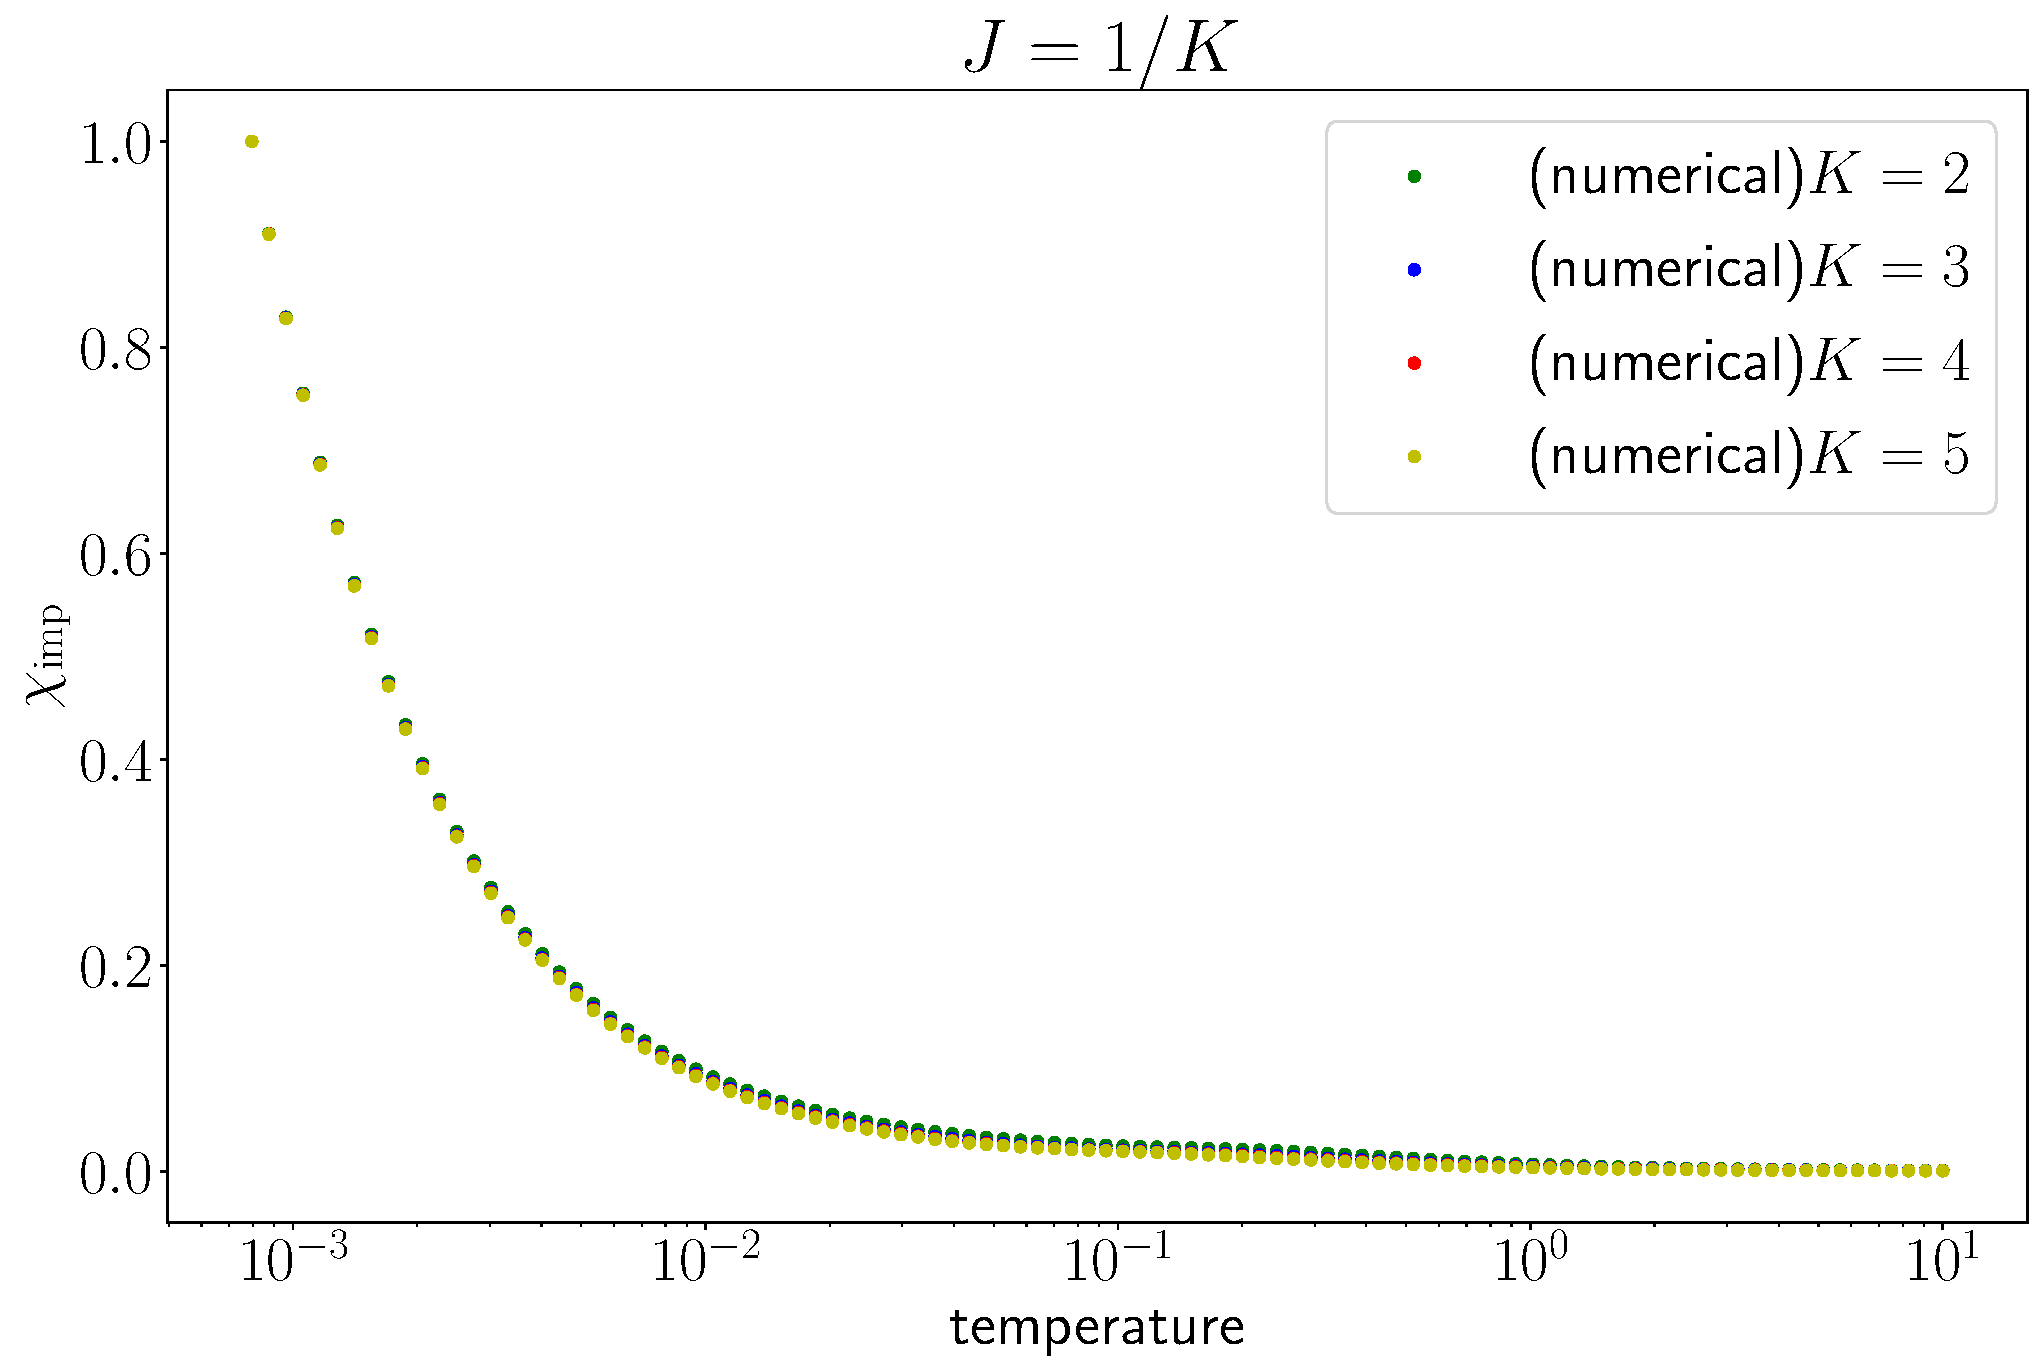
\includegraphics[width=0.8\textwidth]{../numerics/chi_mchannel.pdf}
	\caption{Impurity susceptibility for \(K=1,2,4,6\), calculated numerically as well as using the analytical expressions.}
	\label{chi_mchannel}
\end{figure}

Since the final expressions are formidable, we write down the expressions specifically for the single-channel and two-channel models. For single-channel, we have \(M=\frac{1}{2}\) and \(m = \pm \frac{1}{2}\). The terminal states are \(S_d^z=-\frac{1}{2}, m=-\frac{1}{2}\) and \(S_d^z=\frac{1}{2}, m=\frac{1}{2}\). There is therefore just one \(2\times 2\) block, and that is at \(m=-\frac{1}{2}\).
\begin{gather}
	\lim_{h \to 0}Z(h) = 2e^{\beta \frac{J}{4}}\cosh \beta \frac{J}{2} + 2e^{-\beta \frac{J}{4}} \\
	\lim_{h \to 0}\frac{\:\mathrm{d}Z(h)}{\:\mathrm{d}h} = 0 \\
	\lim_{h \to 0}\frac{\:\mathrm{d}^2Z(h)}{\:\mathrm{d}h^2} = \frac{\beta}{J}\left(e^{\beta \frac{J}{4}}\sinh \beta\frac{J}{2} + e^{-\beta \frac{J}{4}}\frac{J \beta}{2}\right)\\
	\chi = \frac{1}{\beta}\lim_{h \to 0}\left[\frac{Z(h)^{\prime\prime}}{Z(h)} - \left(\frac{Z(h)^{\prime}}{Z(h)}\right)^2 \right] = \frac{1}{J}\frac{\left(2e^{\beta \frac{J}{2}}\sinh \beta\frac{J}{2} + J \beta\right)}{4e^{\beta \frac{J}{2}}\cosh \beta \frac{J}{2} + 4}
\end{gather}
This expression matches with the direct calculation of the susceptibility of the single-channel Kondo model.

At low temperature \(\beta \to \infty\), only the highest value \(M_\text{max}\) will survive:
\begin{align}
	Z &\to 2 r^K_{M_\text{max}} M_\text{max} e^{\beta \frac{J}{2}(M_\text{max} + 1)}\\
	Z^{\prime \prime} &\to r^K_{M_\text{max}}\left(\frac{\beta }{2(M_\text{max} + \frac{1}{2})}\right)^2 e^{\beta \frac{J}{2}(M_\text{max} + 1)}\Sigma_\text{max}\\
	\chi &\to \frac{\beta\Sigma_\text{max}}{2M_\text{max}\left(2M_\text{max}+1\right)^2} = \frac{\beta K(K+1)(K-1)/12}{K(K+1)^2} = \frac{\beta(K-1)}{12(K+1)}
\end{align}

At high temperatures \(\beta \to 0\), we get
\begin{align}
	Z &\to \sum_{M=M_\text{min}}^{M_\text{max}}r^K_M\left[4M + 2\right]\\
	Z^{\prime \prime} &\to \frac{\beta^2}{2}\sum_{M=M_\text{min}}^{M_\text{max}}r^K_M\left[2M + 1\right]\\
	\chi &\to 1/4
\end{align}

\section{Bath Susceptibility from zero-mode fixed point Hamiltonian}
We insert a magnetic field that acts only on the bath and then attempt to diagonalize the Hamiltonian.
\begin{align}
	\label{bath_field_ham}
	H(h) = J^* \vec{S_d}\cdot\vec{s}_\text{tot} + h s^z_\text{tot}
\end{align}

Defining \(x^M_m = M(M+1) - m(m+1)\), the \(2\times 2\) blocks can be written as
\begin{align}
	H_m = \begin{pmatrix} m(\frac{J}{2} + h) & J\sqrt{x^M_m}/2 \\ J\sqrt{x^M_m}/2 & (m+1)(h - \frac{J}{2}) \end{pmatrix} 
\end{align}
The eigenvalues are 
\begin{align}
	\lambda_{m, \pm}^{M, h} &= -\frac{J}{4} + (2m+1)h/2 \pm \frac{1}{2}\sqrt{J^2x^M_m + \left[(2m+1)h - \frac{J}{2}\right]^2 - 4m(m+1)(h^2 - J^2/4)} \nonumber\\
				&= -\frac{J}{4} + (2m+1)h/2 \pm \frac{1}{2}\sqrt{J^2(M + \frac{1}{2})^2 + h^2 - (2m+1)Jh} \nonumber\\
				&= -\frac{J}{4} + (2m+1)h/2 \pm \phi^M_m \label{bath_field_ens}
\end{align}
where \(\phi^M_m = \frac{1}{2}\sqrt{J^2(M + \frac{1}{2})^2 + h^2 - (2m+1)Jh}\).
The eigenvalues of the terminal states are \(JM/2 \pm hM\). The partition function is
\begin{align}
	Z(h) &= \sum_{M=M_\text{min}}^{M_\text{max}}r^K_M\left[\sum_{m=-M, \atop{m\in \mathbb{Z}}}^{M-1}\left(e^{-\beta \lambda_{m, +}^{M, h}} + e^{-\beta \lambda_{m, -}^{M, h}}\right) + e^{-\beta JM/2}\left(e^{\beta hM} + e^{-\beta hM}\right)\right] \\
	     &=\sum_{M=M_\text{min}}^{M_\text{max}}r^K_M\left[\sum_{m=-M, \atop{m\in \mathbb{Z}}}^{M-1}2e^{\beta \left(\frac{J}{4} - (m+\frac{1}{2})h\right)}\cosh \beta\phi^M_m + 2e^{-\beta JM/2}\cosh \beta Mh\right]
\end{align}
We will now take the derivatives.
\begin{align}
	Z^\prime(h) &=\sum_{M=M_\text{min}}^{M_\text{max}}r^K_M\left[\sum_{m=-M, \atop{m\in \mathbb{Z}}}^{M-1}2e^{\beta \left(\frac{J}{4} - (m+\frac{1}{2})h\right)}\left(-\beta (m+\frac{1}{2}) \cosh \beta\phi^M_m + \beta\frac{\:\mathrm{d}\phi^M_m}{\:\mathrm{d}h}\sinh \beta\phi^M_m\right)+ 2\beta Me^{-\beta JM/2}\sinh \beta Mh\right]\\
	Z^{\prime\prime}(h) &=\sum_{M=M_\text{min}}^{M_\text{max}}r^K_M\left[\sum_{m=-M, \atop{m\in \mathbb{Z}}}^{M-1}2 e^{\beta \left(\frac{J}{4} - (m+\frac{1}{2})h\right)}\left(\beta^2 (m+\frac{1}{2})^2 \cosh \beta\phi^M_m - 2\beta^2 (m+\frac{1}{2})\frac{\:\mathrm{d}\phi^M_m}{\:\mathrm{d}h}\sinh \beta\phi^M_m\right.\right.\\
			    &\quad\quad\quad\quad\quad\quad\left.\left. + \beta\frac{\:\mathrm{d^2}\phi^M_m}{\:\mathrm{d}h^2}\sinh \beta\phi^M_m + \beta^2\left(\frac{\:\mathrm{d}\phi^M_m}{\:\mathrm{d}h}\right)^2 \cosh \beta\phi^M_m\right) + 2\beta^2 M^2 e^{-\beta JM/2}\cosh \beta Mh\right]\\
\end{align}
In the limit of \(h \to 0\), we  have
\begin{align}
	     Z(h \to 0) &=\sum_{M=M_\text{min}}^{M_\text{max}}r^K_M\left[\sum_{m=-M, \atop{m\in \mathbb{Z}}}^{M-1}2e^{\beta \frac{J}{4}}\cosh \beta\phi^M_m + 2e^{-\beta JM/2}\right]\\
	Z^\prime(h \to 0) &=\sum_{M=M_\text{min}}^{M_\text{max}}r^K_M\left[\sum_{m=-M, \atop{m\in \mathbb{Z}}}^{M-1}2e^{\beta \frac{J}{4}}\left(-\beta (m+\frac{1}{2}) \cosh \beta\phi^M_m + \beta\frac{\:\mathrm{d}\phi^M_m}{\:\mathrm{d}h}\sinh \beta\phi^M_m\right)\right]\\
	Z^{\prime\prime}(h \to 0) &=\sum_{M=M_\text{min}}^{M_\text{max}}r^K_M\left[\sum_{m=-M, \atop{m\in \mathbb{Z}}}^{M-1}2 e^{\beta \frac{J}{4}}\left(\beta^2 (m+\frac{1}{2})^2 \cosh \beta\phi^M_m - 2\beta^2 (m+\frac{1}{2})\frac{\:\mathrm{d}\phi^M_m}{\:\mathrm{d}h}\sinh \beta\phi^M_m\right.\right.\\
			    &\quad\quad\quad\quad\quad\quad\left.\left. + \beta\frac{\:\mathrm{d^2}\phi^M_m}{\:\mathrm{d}h^2}\sinh \beta\phi^M_m + \beta^2\left(\frac{\:\mathrm{d}\phi^M_m}{\:\mathrm{d}h}\right)^2 \cosh \beta\phi^M_m\right) + 2\beta^2 M^2 e^{-\beta JM/2}\right]\\
\end{align}
The \(\phi\) and the derivatives are actually at \(h\to 0\). We are interested in the low temperature behaviour. In the limit of \(h \to 0\), \(\phi_m^M \to \phi^M = J(M+\frac{1}{2})/2\). We can also look at the behaviour of the derivative:
\begin{align}
	\lim_{h \to 0}\frac{\:\mathrm{d}\phi_m^M}{\:\mathrm{d}h} &= -\frac{J(m+\frac{1}{2})}{4\phi^M}\\
	\lim_{h \to 0}\frac{\:\mathrm{d}^2\phi_m^M}{\:\mathrm{d}h^2} &= \frac{1}{4\phi^M} - \frac{J^2(m + \frac{1}{2})^2}{16\left(\phi^M\right)^3}\\
\end{align}
Substituting these gives
\begin{align}
	     Z(h \to 0) &=\sum_{M=M_\text{min}}^{M_\text{max}}r^K_M\left[\sum_{m=-M, \atop{m\in \mathbb{Z}}}^{M-1}2e^{\beta \frac{J}{4}}\cosh \beta\phi^M + 2e^{-\beta JM/2}\right] = \sum_{M=M_\text{min}}^{M_\text{max}}r^K_M\left[4Me^{\beta \frac{J}{4}}\cosh \beta\phi^M + 2e^{-\beta JM/2}\right]\\
	Z^\prime(h \to 0) &=-\beta\sum_{M=M_\text{min}}^{M_\text{max}}r^K_M2e^{\beta \frac{J}{4}} \left(\cosh \beta\phi^M + \frac{J}{4\phi^M}\sinh \beta\phi^M\right)\sum_{m=-M, \atop{m\in \mathbb{Z}}}^{M-1}\left( m + \frac{1}{2} \right) = 0\\
Z^{\prime\prime}(h \to 0) &=\beta^2\sum_{M=M_\text{min}}^{M_\text{max}}r^K_M\left[2 e^{\beta \frac{J}{4}}\left\{\left(1 + \frac{J^2}{16{\phi^M}^2}\right) \Sigma_M \cosh \beta\phi^M + \left(\frac{2M}{4\beta\phi^M} + \frac{J}{2\phi^M}\left(1 - \frac{J}{16\beta{\phi^M}^2}\right)\Sigma_M \right) \sinh \beta\phi^M\right\} \right.\\
			  &\quad\quad\quad\quad\quad\quad\quad\left.+ 2 M^2 e^{-\beta JM/2}\right]\\
\end{align}
where \(\Sigma_M = \sum_m (m+\frac{1}{2})^2\).

If we take the limit of \(\beta \to \infty\), the hyperbolic functions can be replaced by exponentials. The terms with \(1/\beta\) in \(Z^{\prime\prime}\) drop out. All negative exponentials will also drop out. Moreover, out of all the positve exponentials, only the largest exponent will survive. The largest value \(\Phi\) of \(\phi^M\) occurs at \(M = M_\text{max} = K/2\). This maximum value is \(\Phi = J(K+1)/4\). We therefore have
\begin{align}
	     Z(h \to 0) &= r^K_{K/2} 4Me^{\beta \frac{J}{4}}\frac{1}{2}e^{\beta\Phi}\\
	     Z^{\prime\prime}(h \to 0) &=\beta^2 r^K_{K/2}2 e^{\beta \frac{J}{4}}\frac{1}{2}e^{\beta \Phi}\left(1 + \frac{J}{4\Phi}\right)^2\Sigma_\text{max}\\
\end{align}
The susceptibility at low temperatures becomes
\begin{align}
	\chi(T \to 0) = \frac{2\beta\left(1 + \frac{J}{4\Phi}\right)^2\Sigma_M}{4M} = \frac{\beta (K-1)(K+2)^2}{12(K+1)}
\end{align}

\section{Non-analyticity in the free energy (Discontinuity in magnetization)}

\subsection{Field coupled to impurity}
For \(K>1\), the Gibbs free energy at \(T=0\) becomes non-analytic under insertion of a magnetic field on the impurity. The thermal free energy is given by
\begin{equation}\begin{aligned}
	F(h) = -\frac{1}{\beta}\ln Z(h) = -\frac{1}{\beta}\ln\sum_{E_n}e^{-\beta E_n}
\end{aligned}\end{equation}
At \(T \to 0\), only the most negative energy \(E_\text{min}\) survives. Assuming a non-degenerate ground state for \(h \neq 0\), the zero temperature free energy becomes
\begin{equation}\begin{aligned}
	F(h\neq 0, T\to 0) = -\frac{1}{\beta}\ln e^{-\beta E_\text{min}} = E_\text{min}
\end{aligned}\end{equation}
In the star graph Hamiltonian with \(K-\)channels and in the presence of a field on the impurity (eq.~\ref{stargraph_field_hamiltonian}), the energy eigenvalues for a particular value of \(s_\text{tot}\) are given in eq.~\ref{stargraph_spectrum}. Within a particular subspace \(M\), the ground state energy will be one of the negative eigenvalues:
\begin{equation}\begin{aligned}
	\lambda^{M,h}_{m, -}= -J/4 - \frac{1}{2}\sqrt{J^2x^M_{m}/4 + \alpha^2} = -J/4 - \frac{1}{2}\sqrt{J^2(M+1/2)^2 + h^2 + 2hJ(m+1/2)}
\end{aligned}\end{equation}
The minimum eigenvalue is obtained by maximizing \(h(m+1/2)\). For \(h>0\), the ground state is renormalized for the most positive value of \(m\), \(M-1\). On the other hand, for \(h<0\), it occurs for \(m=-M\), because that is the most negative value it can take. Among all the values of \(M\), the global ground state is at the largest value of \(M\), \(K/2\). Therefore, the minimal energy eigenvalue is
\begin{equation}\begin{aligned}
	E_\text{min}(h) = \begin{cases}
		-J/4 - \frac{1}{2}\sqrt{J^2(K+1)^2/4 + h^2 + hJ(K-1)}, & h>0\\
		-J/4 - \frac{1}{2}\sqrt{J^2(K+1)^2/4 + h^2 - hJ(K-1)}, & h<0\\
	\end{cases}
\end{aligned}\end{equation}
The free energy for a non-zero field is therefore
\begin{equation}\begin{aligned}
	F(h\neq 0, T\to 0) = -J/4 - \frac{1}{2}\sqrt{J^2(K+1)^2/4 + h^2 + |h|J(K-1)}
\end{aligned}\end{equation}
The first derivative of the free energy with respect to the field gives
\begin{equation}\begin{aligned}
	F^\prime(h\neq 0, T\to 0) =- \frac{1}{2}\frac{2h + J(K-1)\text{sign}(h)}{2\sqrt{J^2(K+1)^2/4 + h^2 + |h|J(K-1)}}
\end{aligned}\end{equation}
There we used the result that the derivative of \(|x|\) is \(\text{sign}(x)\). If we now take \(h\) to zero from both directions, we get the magnetization of the impurity
\begin{equation}\begin{aligned}
	m = F^\prime(h \to 0^\pm, T\to 0) = \mp \frac{1}{2}\frac{(K-1)}{(K+1)}
\end{aligned}\end{equation}

The magnetization is therefore discontinuous as \(h\to 0\); it goes to different values depending on the direction in which we take the limit. The only case where it is not analytic is when \(K=1\); then the derivative goes to zero from both directions. This non-analyticity has also been verified numerically.
\begin{figure}[htpb]
	\centering
	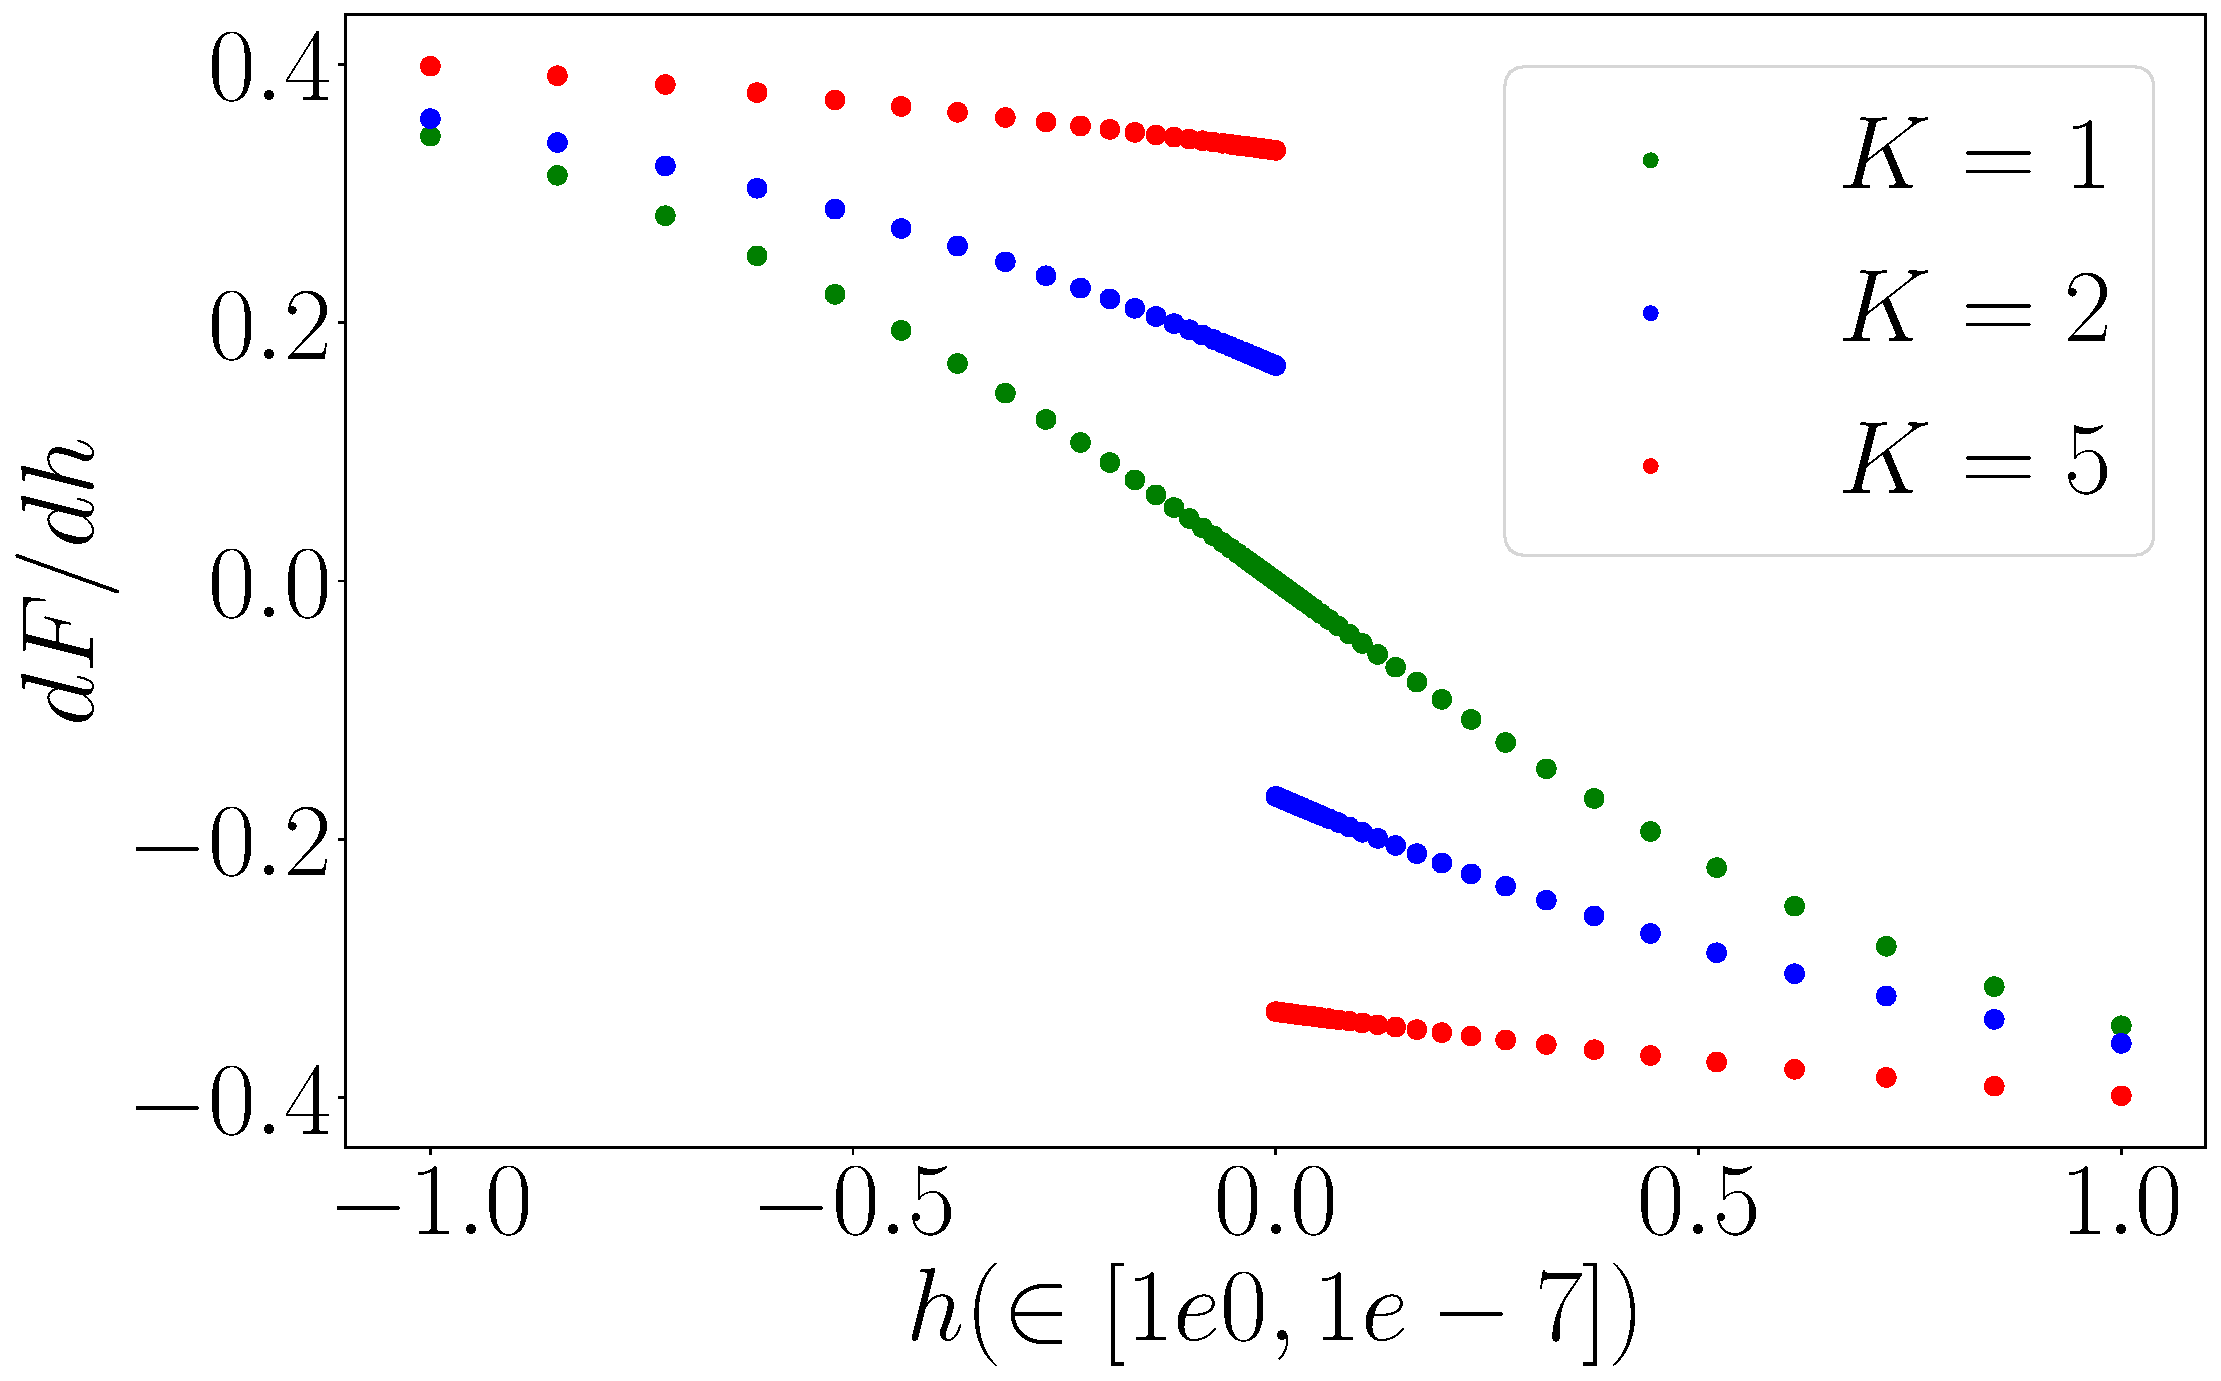
\includegraphics[width=0.6\textwidth]{../numerics/disc_mag_imp.pdf}
	\caption{Non-analytic free energy for \(K>1\) and analytic free energy for \(K=1\).}
\end{figure}

The non-analyticity for \(K>1\) occurs because the magnetic field is able to flip the ground state. For example, for \(K=2\), the states in question are \(\ket{M=1, m=-1,0}\). For \(h>0\), the ground state occurs in the subspace \(\ket{S_d^z=1/2, m=-1},\ket{S_d^z=-1/2,m=0}\). If we now flip the magnetic field, the ground state subspace flips to \(\ket{S_d^z=1/2, m=0},\ket{S_d^z=-1/2,m=1}\). Instead, if we look at the case of \(K=1\), the ground state is in the subspace of \(\ket{S_d^z=1/2,m=-1/2},\ket{S_d^z=-1/2, m=1/2}\), and since there is only this one subspace, the ground state is independent of the field. From this discussion, it is clear that the non-analyticity appears because there are multiple values of \(m \in [-M, M-1]\) in the ground state manifold, which means that it is the ground state degeneracy that causes the non-analyticity.

\subsection{Field coupled to bath zero modes}
Assuming a non-degenerate ground state for \(h \neq 0\), the zero temperature free energy becomes
\begin{equation}\begin{aligned}
	F(h\neq 0, T\to 0) = -\frac{1}{\beta}\ln e^{-\beta E_\text{min}} = E_\text{min}
\end{aligned}\end{equation}
In the star graph Hamiltonian with \(K-\)channels and in the presence of a field on the bath zero modes (eq.~\ref{bath_field_ham}), the energy eigenvalues for a particular value of \(s_\text{tot}\) are given in eq.~\ref{bath_field_ens}. For small field \(h\), the global ground state will lie in the subspace of \(s_\text{tot} = M_\text{max} = K/2\). The ground state energy will be one of the negative eigenvalues:
\begin{equation}\begin{aligned}
	\lambda^{M_\text{max},h}_{m, -} = -J/4 + \left( 2m+1 \right)\frac{h}{2} - \frac{1}{2}\sqrt{J^2(M_\text{max}+\frac{1}{2})^2 + h^2 - \left( 2m+1 \right) Jh}
\end{aligned}\end{equation}
The minimum eigenvalue is obtained by minimizing \(h(2m+1)\). For \(h>0\), the ground state is realized for the most negative value of \(m\), \(-M_\text{max}\). On the other hand, for \(h<0\), it occurs for \(m=M_\text{max}-1\), because that is the most positive value it can take. Therefore, the minimal energy eigenvalue is
\begin{equation}\begin{aligned}
	E_\text{min}(h) = \begin{cases}
		-J/4 - \frac{h}{2}\left(K-1\right) - \frac{1}{2}\sqrt{\frac{1}{4}J^2(K+1)^2 + h^2 + \left(K-1\right) Jh}, & h>0\\
		-J/4 + \frac{h}{2}\left(K-1\right) - \frac{1}{2}\sqrt{\frac{1}{4}J^2(K+1)^2 + h^2 - \left(K-1\right) Jh}, & h<0\\
	\end{cases}
\end{aligned}\end{equation}
The free energy for a non-zero field is therefore
\begin{equation}\begin{aligned}
	F(h\neq 0, T\to 0) = -J/4 - \frac{|h|}{2}\left(K-1\right) - \frac{1}{4}\sqrt{J^2(K+1)^2 + 4h^2 + 4\left(K-1\right) J |h|}
\end{aligned}\end{equation}
The first derivative of the free energy with respect to the field gives
\begin{equation}\begin{aligned}
	F^\prime(h\neq 0, T\to 0) = - \frac{1}{2}(K-1)\text{sign}(h) - \frac{h + \frac{1}{2}J(K-1)\text{sign}(h)}{\sqrt{J^2(K+1)^2 + 4h^2 + 4\left(K-1\right) J |h|}}
\end{aligned}\end{equation}
There we used the result that the derivative of \(|x|\) is \(\text{sign}(x)\). If we now take \(h\) to zero from both directions, we find that the bath magnetization is discontinuous:
\begin{equation}\begin{aligned}
	F^\prime(h \to 0^\pm, T\to 0) = \mp \frac{1}{2}\frac{(K-1)(K+2)}{K+1}
\end{aligned}\end{equation}
\begin{figure}[htpb]
	\centering
	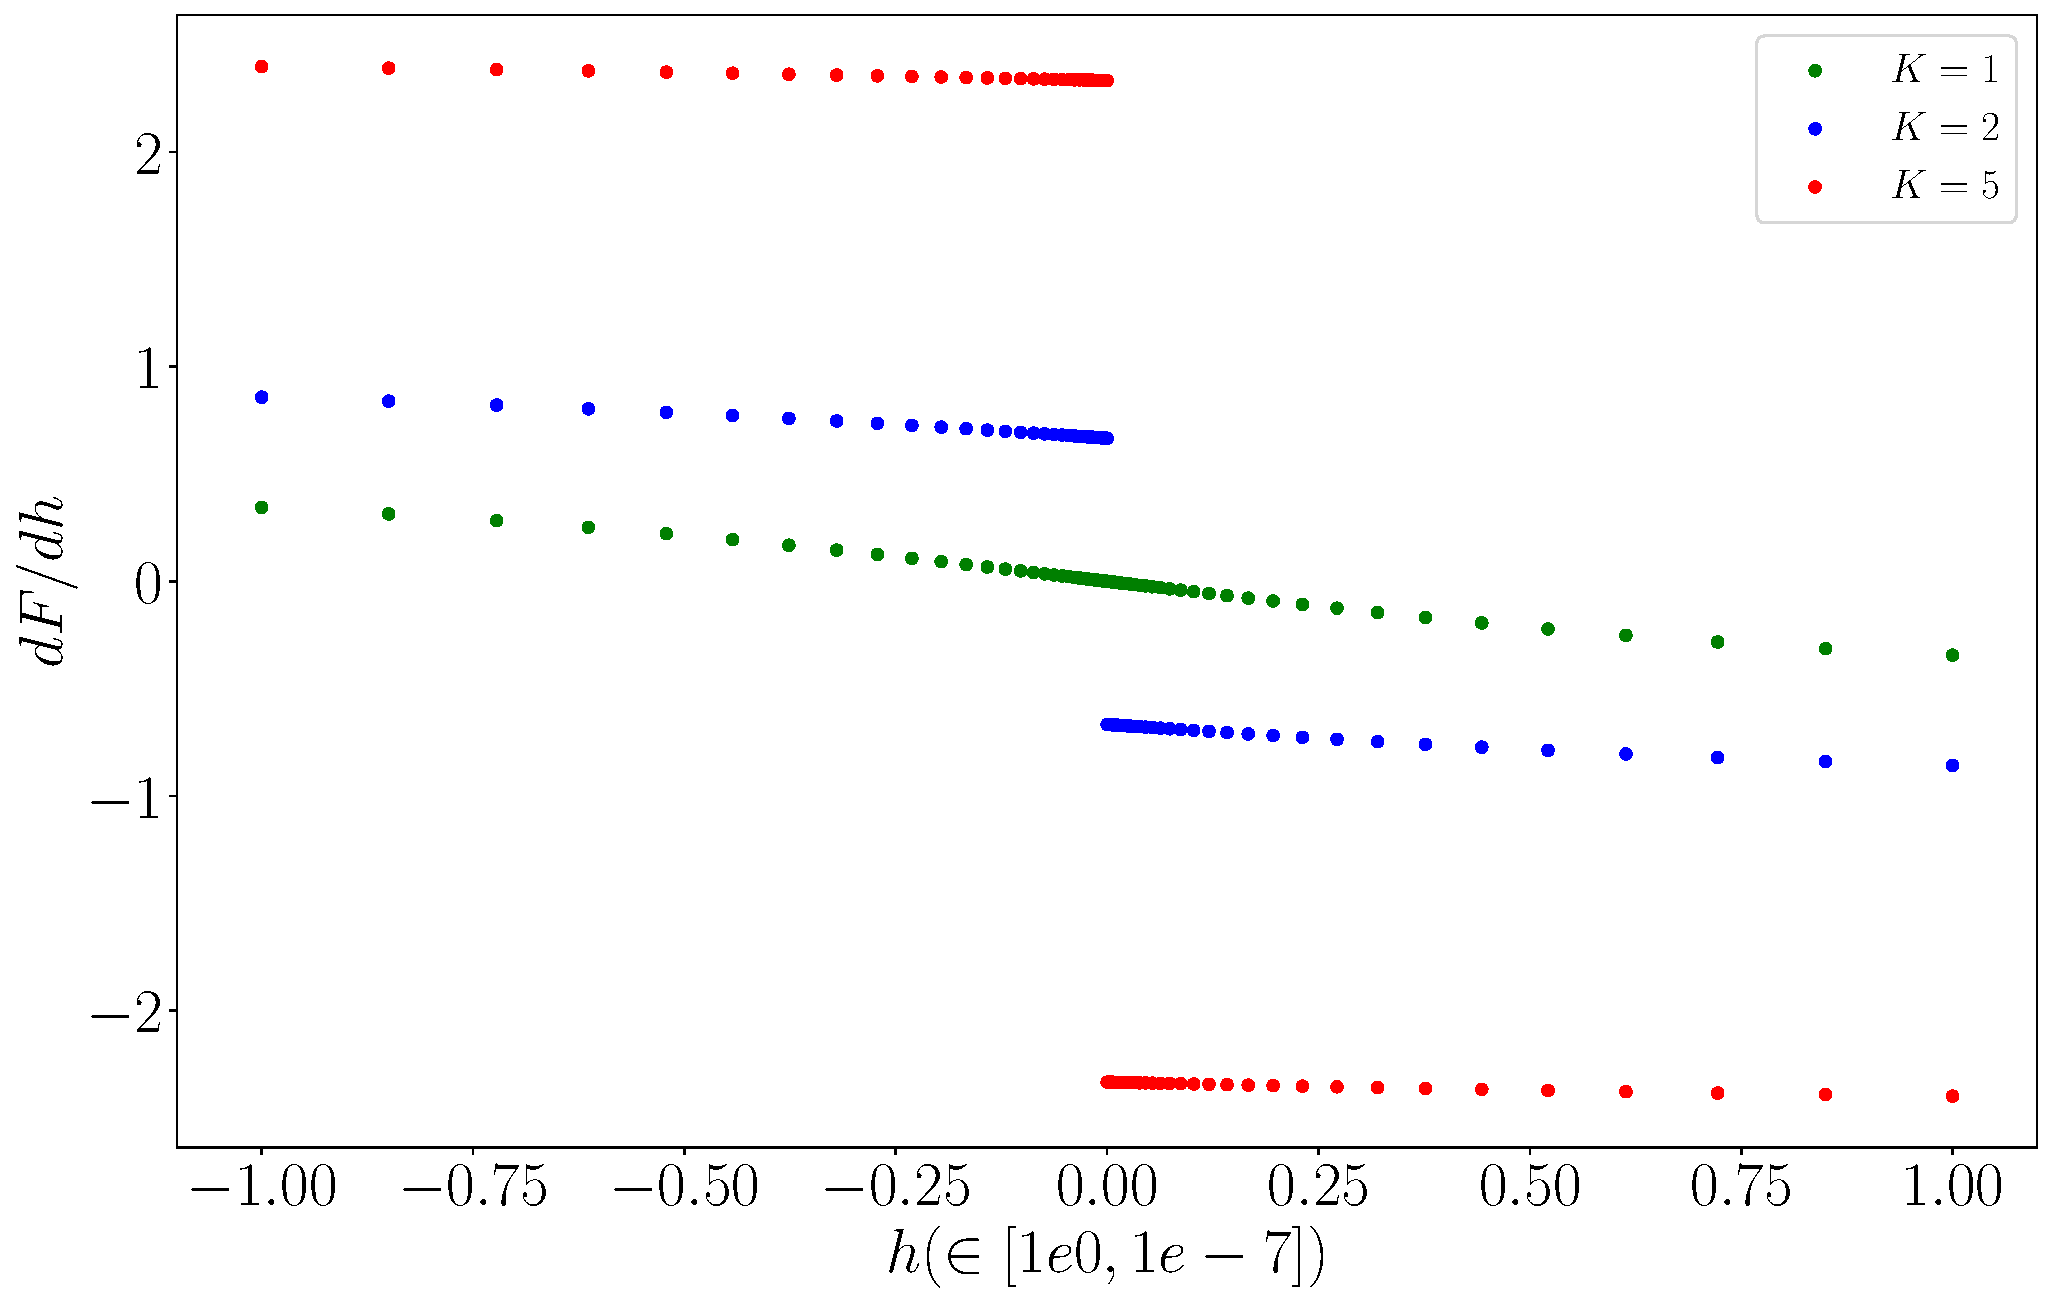
\includegraphics[width=0.6\textwidth]{../numerics/disc_mag_bath.pdf}
	\caption{Non-analytic free energy for \(K>1\) and analytic free energy for \(K=1\).}
\end{figure}

\subsection{Global field}
For \(K>1\), the Gibbs free energy at \(T=0\) becomes non-analytic under insertion of a magnetic field on the impurity. The thermal free energy is given by
\begin{align}
	F(h) = -\frac{1}{\beta}\ln Z(h) = -\frac{1}{\beta}\ln\sum_{E_n}e^{-\beta E_n}
\end{align}
At \(T \to 0\), only the most negative energy \(E_\text{min}\) survives. Assuming a \(d^\prime_\text{gs}-\)fold degenerate ground state for \(h \neq 0\), the zero temperature free energy becomes
\begin{align}
	F(h\neq 0, T\to 0) = -\frac{1}{\beta}\ln d^\prime_\text{gs}e^{-\beta E_\text{min}} = E_\text{min}- k_B T\ln d^\prime_\text{gs}
\end{align}
In the star graph Hamiltonian with \(K-\)channels and a global magnetic field on the impurity
\begin{align}
	H = J \vec{S_d}\cdot\vec{s}_\text{tot} + h\left(S_d^z + s^z_\text{tot}\right) ~,
\end{align}
the energy eigenvalues for a particular value of \(s_\text{tot}=M\) are given by
\begin{align}
	(a) \quad&\frac{J}{2}M \pm h\left(M + \frac{1}{2}\right)\\
	(b) \quad&-\frac{J}{4}\pm \frac{J}{2}\left(M + \frac{1}{2}\right) + h\left( m + \frac{1}{2} \right), m \in \left[-M, M-1\right] 
\end{align}
For small \(h\), the ground state will be \(-\frac{J}{4}- \frac{J}{2}\left(M + \frac{1}{2}\right) + h\left(m_\text{min} + \frac{1}{2} \right)\) for a particular value \(m_\text{min}\) that minimizes this energy. This specific value will depend on the sign of \(h\):
\begin{align}
	m_\text{min} = \begin{cases}
		-M, & h >0\\
		M-1,& h< 0
	\end{cases}
\end{align}
which means \(E_\text{min} = -\frac{J}{2}\left( M + 1 \right) - |h|\left(M - \frac{1}{2}\right)\). We also know, from Eq.~\ref{extra_degen}, that \(d^\prime_\text{gs} = {}^{K-1}C_{K/2 - K/2} = 1\).
The free energy for a non-zero field is therefore
\begin{align}
	F(h\neq 0, T\to 0) = -\frac{J}{2}\left( M + 1 \right) - |h|\left(M - \frac{1}{2}\right)
\end{align}

The first derivative of the free energy with respect to the field gives
\begin{align}
	F^\prime(h\neq 0, T\to 0) = -\text{sign}(h)\left(M - \frac{1}{2}\right)
\end{align}
There we used the result that the derivative of \(|x|\) is \(\text{sign}(x)\). If we now take \(h\) to zero from both directions, we get the total magnetization, and find that it is discontinuous:
\begin{align}
	F^\prime(h \to 0^\pm, T\to 0) = \mp\left(M - \frac{1}{2}\right) = \mp \frac{1}{2}\left( K - 1 \right) 
\end{align}

\begin{figure}[htpb]
	\centering
	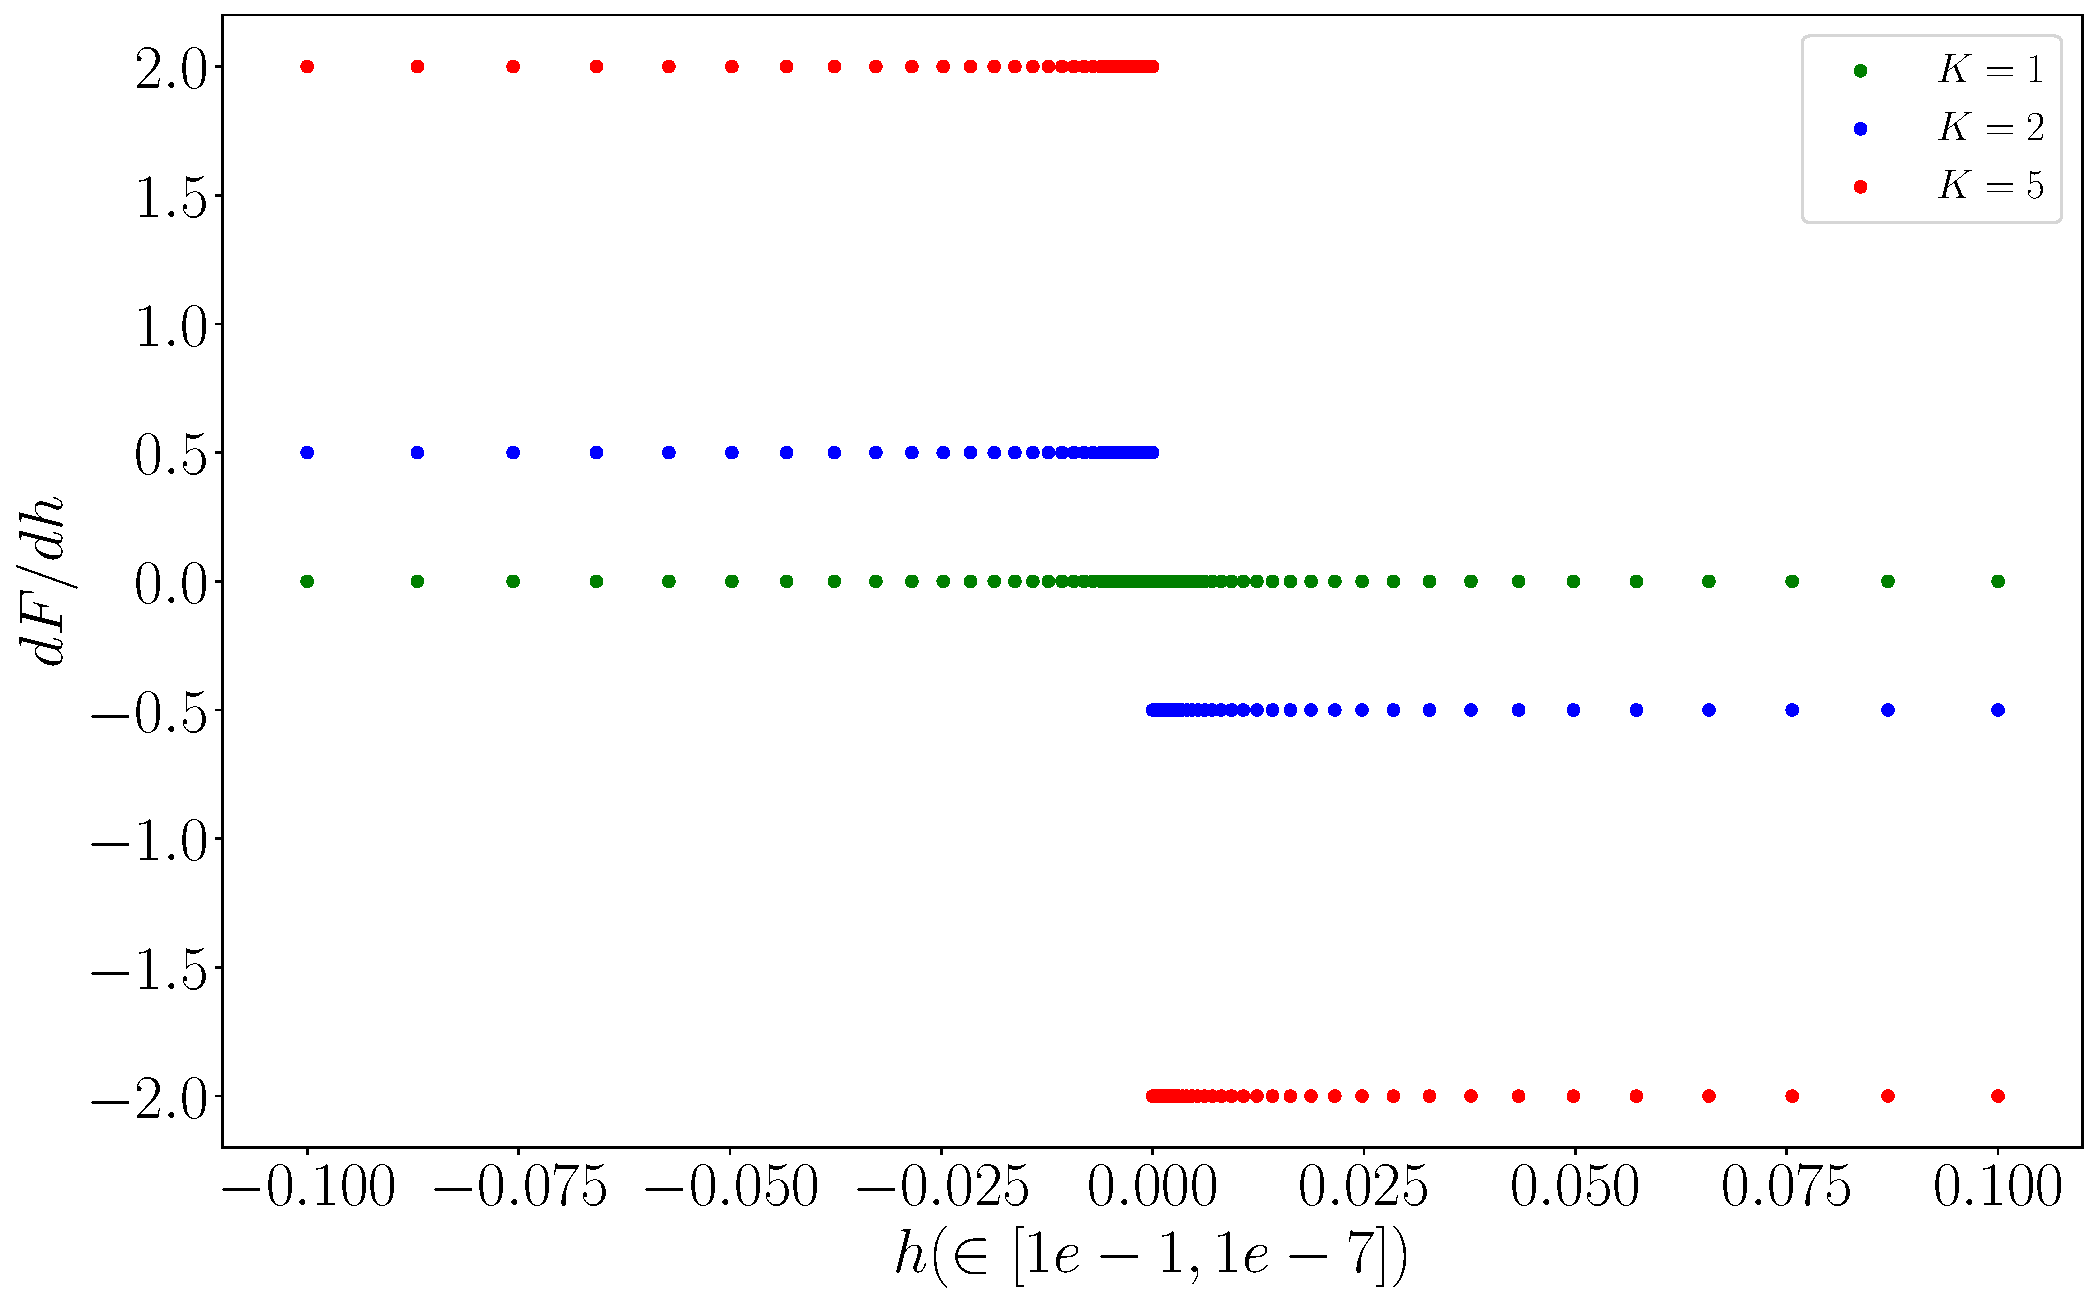
\includegraphics[width=0.6\textwidth]{../numerics/disc_mag_global.pdf}
	\caption{Non-analytic free energy for \(K>1\) and analytic free energy for \(K=1\).}
\end{figure}

\section{Thermal entropy at \(T=0\)}
Given the Helmholtz free energy \(F = -k_B T \ln Z = - \frac{1}{\beta} \ln\sum_n e^{-\beta E_n}\), the thermal entropy at temperature \(T\) is given by
\begin{align}
	S(T) = - \frac{\partial{F}}{\partial{T}} = k_B \ln\sum_n e^{-\beta E_n} + \frac{\sum_n E_n e^{-\beta E_n}}{T \sum_n e^{-\beta E_n}}
\end{align}
In the limit of \(T \to 0\), only the lowest energy state \(E_\text{gs}\) will survive. Assuming this state has a degeneracy \(d_\text{gs}\), we have
\begin{equation}
	S(T \to 0) = k_B \ln\left(d_\text{gs} e^{-\beta E_\text{gs}}\right) + \frac{d_\text{gs} E_\text{gs}e^{-\beta E_\text{gs}}}{T d_\text{gs} e^{-\beta E_\text{gs}}} = k_B \ln d_\text{gs} - \frac{1}{T}E_\text{gs} + \frac{1}{T}E_\text{gs} = k_B \ln d_\text{gs}
\end{equation}
This is a general result that holds for any system with a \(d_\text{gs}\)-fold degenerate ground state. For the star graph problem, we have a \(K-\)fold degenerate ground state, so the \(T=0\) entropy of the star graph Hamiltonian with \(K\) outer spins is \(S(T\to 0) = k_B \ln K\). The impurity contribution to the total entropy is obtained by subtracting the entropy of the non-interacting bath. But we know that the entropy of a free Fermi gas vanishes at low temperatures. The impurity contribution is therefore
\begin{equation}
	\label{res_entropy}
	S_\text{imp}(T\to 0) = k_B \ln K
\end{equation}

We wish to point out that this value is different from the more commonly cited result \(S = \ln 2\cos \frac{\pi}{K+2}\) obtained from other methods like the Bethe ansatz (BA) and conformal field theory (CFT) calculations~\cite{Gan_Andrei_Coleman_1993,andrei_destri_1984,Tsvelick_weigmann_mchannel_1985,sacramento1989,emery_kivelson,affleck_1991_overscreen}. The difference is not only in the value but also in the origin. Eq.~\ref{res_entropy} describes the thermal entropy coming purely from the quantum mechanical degeneracy of the star graph problem (which is the star graph of the full MCK problem), while the second result presumably arises from the zero-modes of the lowest-lying excitations above the star graph ground state, arising from a thermodynamically-large continuous bath with Dirac-like linear dispersion. Another difference is that while Eq.~\ref{res_entropy} holds true independent of system size, the second result is obtained only if the limit of system size \(L \to \infty\) is taken prior to taking the limit of temperature \(T \to 0\)~\cite{Gan_Andrei_Coleman_1993,rozhkov_1998,vondelft_prl_1998}. We note however that the entropy coming from the degeneracy is larger than that coming from the excitations (fig.~\ref{entropy_comparison}), and consequently plays a very important role in the physics of the MCK problem, being responsible for the NFL physics and the critical behaviour near the fixed point.
\begin{figure}[!htpb]
	\centering
	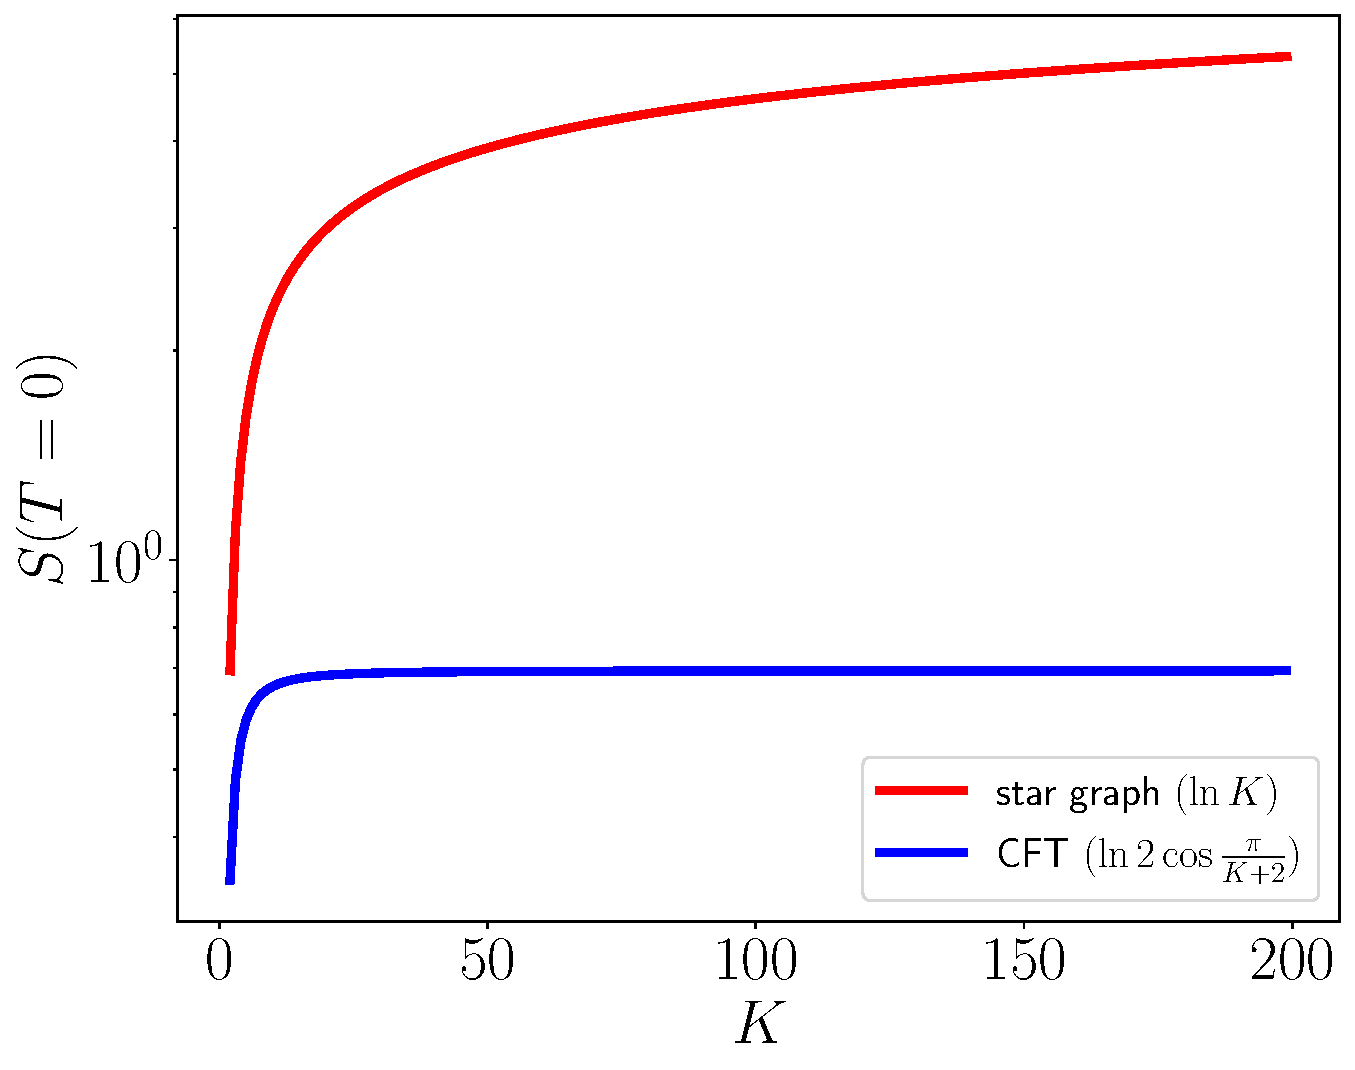
\includegraphics[width=0.5\textwidth]{../numerics/entropy_comparison.pdf}
	\caption{Comparison of star graph zero temperature entropy with CFT/Bethe ansatz formula}
	\label{entropy_comparison}
\end{figure}

\appendix
\section{URG equations for the single-channel Kondo model}
The single-channel SU(2) Kondo model consists of a spin-half impurity interacting with a band of itinerant conduction electrons through a spin-exchange coupling:
\begin{align}
\label{1KondoURG}
	\mathcal{H} = \sum_{k\sigma}\epsilon_{k}\tau_{k\sigma} + \sum_{kl} J^z S_d^z s^z_{kl} + \frac{1}{2}\sum_{kl} J^t \left(S_d^+ s^-_{kl}  + S_d^- s^+_{kl}\right)
\end{align}
Here, \(s^z_{kl} = \frac{1}{2}\left(c^\dagger_{k\uparrow}c_{l \uparrow} - c^\dagger_{k\downarrow}c_{l \downarrow}\right)\), \(s^-_{kl} = c^\dagger_{k \downarrow}c_{l \uparrow}\) and \(s^+_{kl} = {s^-_{lk}}^\dagger\). Also, \(\tau = \hat n - \frac{1}{2}\). The indices \(k,l\) sum over the momentum states. \(\vec S_d\) is the impurity spin operator with \(S_d^z = \pm \frac{1}{2}\).

The scheme is that we will disentangle an electron \(q\beta\) from the Hamiltonian, \(q\) being the momentum and \(\beta\) the spin. The diagonal part of the Hamiltonian under this scheme is
\begin{align}
\label{kondodiag}
H^D_{q\beta} = \epsilon_q \tau_{q\beta} + J^z S_d^z s_{qq}^z
\end{align}
The off-diagonal parts at a particular RG step \(H^I_1\) and \(H^I_0\), that start from particle and hole states respectively, are
\begin{align}
	H^I_1 = \sum_{|k|<\Lambda,q} J^z S_d^z s^z_{kq} + \frac{1}{2}\sum_{|k|<\Lambda,q} J^t \left(S_d^+ s^-_{kq} + S_d^- s^+_{kq}\right)\\
	H^I_0 = \sum_{|k|<\Lambda,q} J^z S_d^z s^z_{qk} + \frac{1}{2}\sum_{|k|<\Lambda,q} J^t \left(S_d^+ s^-_{qk}  + S_d^- s^+_{qk}\right)
\end{align}
\(H^I_1\) is the Hamiltonian term that scatters from the occupied configuration of \(q\), \(H^I_0\) is the same from the unoccupied configuration.
These are the terms that appear in the numerator.
\subsection{Particle sector}
The particle sector involves integrating out those states which are occupied (\(\hat n_{q\beta}=1\)). We will work at an energy  shell \(\epsilon_q = -D\). The renormalization is
\begin{align}
	H^I_0 \frac{1}{\omega - H^D_{q\beta}} H^I_1
\end{align}

Both \(H^I_0\) and \(H^I_1\) have all three operators \(S_d^z, S_d^\pm\). The entire product will thus have \(3\times 3 = 9\) terms. Not all terms however renormalize the Hamiltonian. Those terms that have identical operators on both sides can be ignored because \({S_d^z}^2 = \text{constant}\) and \({S^\pm}^2 = 0\). The other six terms will renormalize the Hamiltonian. This brings in one more simplification: all the six terms that \textit{will} renormalize the Hamiltonian have a spin flip operator on at least one side of the Greens function. This means that in the denominator of the Greens function, \(S_d^z\) and \(s^z_{qq}\) have to be anti-parallel in order to produce a non-zero result for that term. This means we can identically replace \(S_d^z s^z_{qq} = -\frac{1}{4}\). Also, in the particle sector, the Greens function always has \(c_{q\beta}\) in front of it, so \(\epsilon_q \tau_{q\beta} = \frac{D}{2}\). Substituting all this, we get
\begin{align}
	\frac{1}{\omega - \frac{D}{2} + \frac{J}{4}}\sum_{|k,k^\prime|<\Lambda,q}\left[\frac{1}{2}J^z J^t \left(S_d^z S_d^+ s^z_{qk^\prime}s^-_{kq} + S_d^z S_d^- s^z_{qk^\prime}s^+_{kq}\right) + \frac{1}{2}J^t J^z \left(S_d^+ S_d^z s^-_{qk^\prime}s^z_{kq} + S_d^- S_d^z s^+_{qk^\prime}s^z_{kq}\right)\right.\\
+\left.\frac{1}{4}{J^t}^2 \left(S_d^- S_d^+ s^+_{qk^\prime}s^-_{kq} + S_d^+ S_d^- s^-_{qk^\prime}s^+_{kq}\right)\right]
\end{align}
We now simplify the products and keep only terms diagonal in \(q\). For example: \(s^z_{qk^\prime}s^+_{kq} = \frac{1}{2}\hat n_{q \downarrow}s^+_{kk^\prime}\) and \(s^z_{qk^\prime}s^-_{kq} = -\frac{1}{2}\hat n_{q \uparrow}s^-_{kk^\prime}\). The renormalization becomes
\begin{align}
	\frac{1}{\omega - \frac{D}{2} + \frac{J}{4}}\sum_{|k,k^\prime|<\Lambda,q}\left[\frac{1}{4}J^z J^t \left(-\frac{1}{2}S_d^+ \hat n_{q}s^-_{kk^\prime} - \frac{1}{4}S_d^- \hat n_{q} s^z_{kk^\prime}\right) - \frac{1}{4}{J^t}^2 S_d^z\left(-\hat n_{q \uparrow}c^\dagger_{k \downarrow}c_{k^\prime \downarrow} + \hat n_{q \downarrow}c^\dagger_{k \uparrow}c_{k^\prime \uparrow}\right)\right]
\end{align}
We now replace \(\sum_q \hat n_{q\sigma} = n(D)\). The renormalization due to excitations coming from the particle sector is
\begin{align}
	\Delta H_1 = -\frac{1}{2}\frac{n(D)}{\omega - \frac{D}{2} + \frac{J}{4}}\sum_{|k,k^\prime|<\Lambda}\left[J^z J^t \frac{1}{2}\left(S_d^+ s^-_{kk^\prime} + S_d^- s^z_{kk^\prime}\right) + {J^t}^2 S_d^z s^z_{kk^\prime}\right]
\end{align}
The renormalization in the couplings coming from the particle sector is therefore,
\begin{align}
	\label{kondo_part}
	\Delta J^z = -\frac{1}{2}\frac{{J^t}^2n(D)}{\omega - \frac{D}{2} + \frac{J}{4}}, && \Delta J^t = -\frac{1}{2}\frac{J^z J^tn(D)}{\omega - \frac{D}{2} + \frac{J}{4}}
\end{align}


\subsection{Hole sector}
The hole sector involves integrating out those states which are vacant (\(\hat n_{q\beta}=1\)). We will work at an energy  shell \(\epsilon_q = D\). The renormalization is
\begin{align}
	H^I_1 \frac{1}{\omega - H^D_{q\beta}} H^I_0
\end{align}
The same considerations as those in the particle sector apply here, and the denominator becomes \(\omega - \frac{D}{2} + \frac{J}{4}\), while the numerator is \(H^I_1 H^I_0\). Since this is just the Hermitian conjugate of the particle sector form, we do not need to calculate this separately, because the renormalization here will be \(\Delta H_0 = \Delta H_1^\dagger = \Delta H_1\).

\subsection{Scaling equations}
Since the renormalization in the hole sector is equal to that in the particle sector, the total renormalization is simply twice that in the particle sector (eqs.~\ref{kondo_part}):
\begin{align}
	\Delta J^z = -\frac{{J^t}^2n(D)}{\omega - \frac{D}{2} + \frac{J}{4}}, && \Delta J^t = -\frac{J^z J^tn(D)}{\omega - \frac{D}{2} + \frac{J}{4}}
\end{align}
If we set \(J_z = J_t = J\), we have an SU(2)-symmetric Kondo model \(J \vec{S_d}\cdot\vec{s}\).
\begin{align}
	\label{kondosym}
	\Delta J = - \frac{J^2 n(D)}{\omega - \frac{D}{2} + \frac{1}{4}J}
\end{align}
To recover the one-loop form, we can replace \(\omega\) with the bare value \(-\frac{D}{2}\) and ignore the \(J\) in the denominator (small \(J\)).
\begin{align}
	\Delta J \approx \frac{J^2 n(D)}{D}
\end{align}
\begin{align}
	\Delta J^{(2)} = -\frac{J^2 n(D)}{\omega - \frac{D}{2} + \frac{J}{4}}
\end{align}
For \(\omega < \frac{D}{2}\), we get the flow towards the strong coupling fixed point. That is, there appears a stable fixed point at \(J^* = 4|\omega - \frac{D}{2}|\) for all bare \(J > 0\). We also get a decay towards the local moment fixed point \(J^* = 0\) for \(J < 0\). For \(\omega = -\frac{D}{2}\) and \(J \ll D\), we get the one-loop PMS form. 
\begin{align}
	\Delta J^{(2)} = \frac{J^2 n(D)}{D - \frac{J}{4}} \simeq \frac{J^2 n(D)}{D}
\end{align}

\section{URG equations for the single-channel Kondo model with spin-\(S\) impurity}
The Hamiltonian is the same as eq.~\ref{1KondoURG}, but the impurity is now a spin-\(S\) object, such that \(S_d^z \in \left[-S, -S+1,\ldots,S-1,S\right] \).
\begin{equation}\begin{aligned}
	\mathcal{H} = \sum_{k\sigma}\epsilon_{k}\tau_{k\sigma} + \sum_{kl} J S_d^z s^z_{kl} + \frac{1}{2}\sum_{kl} J \left(S_d^+ s^-_{kl}  + \text{h.c.}\right)
\end{aligned}\end{equation}
It is easier to see the RG flow of the couplings if we write the Hamiltonian in terms of the eigenstates of \(S_d^z\). These eigenstates are defined by \(S_d^z\ket{m} = m\ket{m}, m \in \left[-S, S\right]\). In terms of these eigenstates, the Hamiltonian becomes
\begin{equation}\begin{aligned}
	\mathcal{H} &= \sum_{k\sigma}\epsilon_{k}\tau_{k\sigma} + \sum_{kl} J S_d^z\sum_m \ket{m}\bra{m} s^z_{kl} + \frac{1}{2}\sum_{kl} J \left(S_d^+ s^-_{kl}  + \text{h.c.}\right)\sum_m \ket{m}\bra{m} \\
		    &= \sum_{k\sigma}\epsilon_{k}\tau_{k\sigma} + \sum_{m=-S}^S \sum_{kl,\atop{\sigma=\uparrow,\downarrow}} J^\sigma_m \ket{m}\bra{m} c^\dagger_{k \sigma}c_{l \sigma} + \sum_{kl} \sum_{m=-S}^{S-1} J^t_{m} \left(\ket{m+1}\bra{m} s^-_{kl}  + \text{h.c.}\right)
\end{aligned}\end{equation}
where \(J^\sigma_m = \frac{1}{2} \sigma m J\) in the UV Hamiltonian, and \(J^t_{m} = J\frac{1}{2}\sqrt{S(S+1) - m(m+1)}\) is the coupling that connects \(\ket{m}\) and \(\ket{m+1}\).

The various terms that renormalize the Hamiltonian can be described in terms of the bath spin operators that come into them. For example, the term that has \(s^z\) on both sides of the intervening Greens function can be represented as \(z|z\). There are 7 such terms: \(z|z, \pm|\mp, z|\pm, \pm|z\). Each of these terms occur both in the particle and the hole sectors.

\subsection{Particle sector}
We will now calculate each of these terms for the particle sector. The particle sector consists of those processes that start from an occupied state \(\left(\hat n_{q\beta} = 1\right)\).
\paragraph{\(z|z\)}
\begin{equation}\begin{aligned}
	\sum_{kk^\prime,m,\sigma} c^\dagger_{q \sigma} c_{k^\prime \sigma} \ket{m}\bra{m}\frac{{J^\sigma_m}^2}{\omega - \frac{D}{2} + \frac{J}{2}\sigma S_d^z}\ket{m}\bra{m} c^\dagger_{k \sigma}c_{q \sigma} = -\sum_{kk^\prime,m,\sigma}n_{q \sigma}\frac{{J^\sigma_m}^2 c^\dagger_{k \sigma}c_{k^\prime\sigma} \ket{m}\bra{m}}{\omega_{m, \sigma} - \frac{D}{2} + \frac{J}{2}\sigma m}
\end{aligned}\end{equation}

\paragraph{\(+|-\)}
\begin{equation}\begin{aligned}
	\sum_{kk^\prime,m} c^\dagger_{q \uparrow} c_{k^\prime \downarrow} \ket{m}\bra{m+1}\frac{{J^t_m}^2}{\omega - \frac{D}{2} + \frac{J}{2}S_d^z}\ket{m+1}\bra{m} c^\dagger_{k \downarrow}c_{q \uparrow} = -n_{q \uparrow}\sum_{kk^\prime,m}\frac{{J^t_m}^2 c^\dagger_{k \downarrow}c_{k^\prime\downarrow} \ket{m}\bra{m}}{\omega_{m+1, \uparrow} - \frac{D}{2} + \frac{J}{2}\left( m+1 \right) }
\end{aligned}\end{equation}

\paragraph{\(-|+\)}
\begin{equation}\begin{aligned}
	\sum_{kk^\prime,m} c^\dagger_{q \downarrow} c_{k^\prime \uparrow} \ket{m+1}\bra{m}\frac{{J^t_m}^2}{\omega - \frac{D}{2} - \frac{J}{2}S_d^z}\ket{m}\bra{m+1} c^\dagger_{k \uparrow}c_{q \downarrow} = -n_{q \downarrow}\sum_{kk^\prime,m}\frac{{J^t_m}^2 c^\dagger_{k \uparrow}c_{k^\prime\uparrow} \ket{m+1}\bra{m+1}}{\omega_{m, \downarrow} - \frac{D}{2} - \frac{J}{2}m}
\end{aligned}\end{equation}

\paragraph{\(z|+\)}
\begin{equation}\begin{aligned}
	\sum_{kk^\prime,m} c^\dagger_{q \downarrow} c_{k^\prime \downarrow} \ket{m}\bra{m}\frac{J^\downarrow_m{J^t_m}}{\omega - \frac{D}{2} - \frac{J}{2}S_d^z}\ket{m}\bra{m+1} c^\dagger_{k \uparrow}c_{q \downarrow} = -n_{q \downarrow}\sum_{kk^\prime,m}\frac{J^\downarrow_m J^t_m c^\dagger_{k \uparrow}c_{k^\prime\downarrow} \ket{m}\bra{m+1}}{\omega_{m, \downarrow} - \frac{D}{2} - \frac{J}{2}m}
\end{aligned}\end{equation}

\paragraph{\(+|z\)}
\begin{equation}\begin{aligned}
	\sum_{kk^\prime,m} c^\dagger_{q \uparrow}c_{k^\prime \downarrow} \ket{m}\bra{m+1}\frac{{J^t_m}J^\uparrow_{m+1}}{\omega - \frac{D}{2} + \frac{J}{2}S_d^z} \ket{m+1}\bra{m+1} c^\dagger_{k \uparrow} c_{q \uparrow} = -n_{q \uparrow}\sum_{kk^\prime,m}\frac{J^\uparrow_{m+1} J^t_m c^\dagger_{k \uparrow}c_{k^\prime\downarrow} \ket{m}\bra{m+1}}{\omega_{m+1, \downarrow} - \frac{D}{2} + \frac{J}{2}\left(m+1\right) }
\end{aligned}\end{equation}

\paragraph{\(z|-\)}
\begin{equation}\begin{aligned}
	\sum_{kk^\prime,m} c^\dagger_{q \uparrow} c_{k^\prime \uparrow} \ket{m+1}\bra{m+1}\frac{J^\uparrow_{m+1}{J^t_m}}{\omega - \frac{D}{2} + \frac{J}{2}S_d^z}\ket{m+1}\bra{m} c^\dagger_{k \downarrow}c_{q \uparrow} = -n_{q \uparrow}\sum_{kk^\prime,m}\frac{J^\uparrow_{m+1} J^t_m c^\dagger_{k \downarrow}c_{k^\prime\uparrow} \ket{m+1}\bra{m}}{\omega_{m+1, \uparrow} - \frac{D}{2} + \frac{J}{2}(m+1)}
\end{aligned}\end{equation}

\paragraph{\(-|z\)}
\begin{equation}\begin{aligned}
	\sum_{kk^\prime,m} c^\dagger_{q \downarrow} c_{k^\prime \uparrow} \ket{m+1}\bra{m}\frac{J^\downarrow_{m}{J^t_m}}{\omega - \frac{D}{2} - \frac{J}{2}S_d^z}\ket{m}\bra{m} c^\dagger_{k \downarrow}c_{q \downarrow} = -n_{q \downarrow}\sum_{kk^\prime,m}\frac{J^\downarrow_{m} J^t_m c^\dagger_{k \downarrow}c_{k^\prime\uparrow} \ket{m+1}\bra{m}}{\omega_{m, \downarrow} - \frac{D}{2} - \frac{J}{2}(m)}
\end{aligned}\end{equation}
To compare with the spin-\(\frac{1}{2}\) RG equations, we will transform the general spin-\(S\) \(\omega\) to the spin-\(\frac{1}{2}\) \( \omega\), using \(\omega_{m,\sigma} \to \omega - \frac{J}{2}\left(m\sigma - \frac{1}{2}\right)\).
The first four terms renormalize \(J^\sigma_m\):
\begin{equation}\begin{aligned}
	\Delta J^\sigma_{m} = -\frac{\left( J^\sigma_m \right) ^2 + \left( J^t_{m-\frac{1+\sigma}{2}} \right) ^2}{\omega - \frac{D}{2} + \frac{J}{4}}
\end{aligned}\end{equation}
Here, we have defined \(J^t_m = 0\) for \( |m| > S\). Two relations can be obtained from this RG equation, the RG equations for the sum and difference of the couplings. These sum and difference are defined by rewriting the Ising part of the Hamiltonian in the following fashion:
\begin{equation}\begin{aligned}
	\sum_{m=-S}^S \sum_{kl,\atop{\sigma=\uparrow,\downarrow}} J^\sigma_m \ket{m}\bra{m} c^\dagger_{k \sigma}c_{l \sigma} = \sum_{m=-S}^S \sum_{\sigma=\uparrow,\downarrow} J^+_m \ket{m}\bra{m} \sum_\sigma \hat n_{0\sigma}  + \sum_{m=-S}^S J^-_m \ket{m}\bra{m} 2s^z_0
\end{aligned}\end{equation}
where \(2J^\pm_m = J^\uparrow_m \pm J^\downarrow_m\).
The RG equation for the sum of the couplings is
\begin{equation}\begin{aligned}
	\Delta J^+_m = -\frac{1}{2}\frac{\sum_\sigma \left( J^\sigma_m \right) ^2 + \sum_\sigma \left( J^t_{m-\frac{1+\sigma}{2}} \right) ^2}{\omega - \frac{D}{2} + \frac{J}{4}} = -\frac{J^2}{4}\frac{S(S+1)}{\omega - \frac{D}{2} + \frac{J}{4}}
\end{aligned}\end{equation}
This is an \(m-\)independent piece, so it can be summed over to produce an impurity-independent potential scattering term:
\begin{equation}\begin{aligned}
	\sum_{m=-S}^S \sum_{\sigma=\uparrow,\downarrow} J^+ \ket{m}\bra{m} \sum_\sigma \hat n_{0\sigma} = J^+ \mathbb{I}\sum_\sigma \hat n_{0\sigma}
\end{aligned}\end{equation}
Since this term does not have any Kondo physics, we drop this piece and say that \(\Delta J^+ = 0\) and so \(\Delta J^\uparrow_m = - \Delta J^\downarrow_m \implies J^\uparrow_m = -J^\downarrow_m\) throughout the RG flow.

The second is the RG equation for the difference of the couplings:
\begin{equation}\begin{aligned}
	\Delta J^-_m = -\frac{1}{2}\frac{\left( J^t_{m-1} \right) ^2 - \left(J^t_{m}\right) ^2}{\omega - \frac{D}{2} + \frac{J}{4}} = -\frac{1}{4}\frac{m J^2}{\omega - \frac{D}{2} + \frac{J}{4}}
\end{aligned}\end{equation}
The usual \(J^z\) Kondo coupling is defined as \(J^z = 2J^-_m/m\). Substituting this gives 
\begin{equation}\begin{aligned}
	\Delta J^z = -\frac{1}{2}\frac{J^2}{\omega - \frac{D}{2} + \frac{J}{4}}
\end{aligned}\end{equation}

The last four terms renormalize \(J^t_m\):
\begin{equation}\begin{aligned}
	\Delta J^t_m = - \frac{J^t_m \left( J^\downarrow_m + J^\uparrow_{m+1} \right) }{\omega - \frac{D}{2} + \frac{J}{4}} = -\frac{1}{2}\frac{J^t_m J}{\omega - \frac{D}{2} + \frac{J}{4}} \implies J^t = -\frac{1}{2}\frac{J^2}{\omega - \frac{D}{2} + \frac{J}{4}}
\end{aligned}\end{equation}
\(J^t\) is the transverse coupling. Since we started from an isotropic model \(\left( J^z = J^t= J \right) \), we obtain \(\Delta J^z = \Delta J^t\).

\subsection{Hole sector}
The RG equation in this sector is identical to that in the hole sector, because the renormalization terms are Hermitian conjugate to this in the particle sector.

\bibliographystyle{apsrev4-1}
\bibliography{mck_urg}

\end{document}
